\documentclass[a4paper,german]{scrreprt}

% Uncomment to optimize for double-sided printing.
% \KOMAoptions{twoside}

% Set binding correction manually, if known.
% \KOMAoptions{BCOR=2cm}

% Localization options
\usepackage[german]{babel}
\usepackage[T1]{fontenc}
\usepackage[utf8]{inputenc}

% Enhanced verbatim sections. We're mainly interested in
% \verbatiminput though.
\usepackage{verbatim}

% PDF-compatible landscape mode.
% Makes PDF viewers show the page rotated by 90°.
\usepackage{pdflscape}

% Advanced tables
\usepackage{tabu}
\usepackage{longtable}
\usepackage{dcolumn}
\newcolumntype{d}[1]{D{.}{\cdot}{#1} }

% Fancy tablerules
\usepackage{booktabs}

% Graphics
\usepackage{graphicx}

% Current time
\usepackage[useregional=numeric]{datetime2}

% Float barriers.
% Automatically add a FloatBarrier to each \section
\usepackage[section]{placeins}

% Custom header and footer
\usepackage{fancyhdr}

\usepackage{geometry}
\usepackage{layout}

% Math tools
\usepackage{mathtools}
% Math symbols
\usepackage{amsmath,amsfonts,amssymb}
\usepackage{amsthm}

% SI units
\usepackage{siunitx}
\DeclareSIUnit\Molar{\textsc{m}}

% Chemistry
\usepackage{mhchem}

% Subfigures & captions
\usepackage{subcaption}

\DeclarePairedDelimiter\abs{\lvert}{\rvert}

\pagestyle{plain}
% \fancyhf{}
% \lhead{}
% \lfoot{}
% \rfoot{}
% 
% Source code & highlighting
\usepackage{listings}

% Convenience commands
\newcommand{\mailsubject}{2027 - Praktikum Biochemie 1}
\newcommand{\maillink}[1]{\href{mailto:#1?subject=\mailsubject}
                               {#1}}

% Should use this command wherever the print date is mentioned.
\newcommand{\printdate}{\today}

\subject{2027 - Praktikum Biochemie 1}
\title{6 - Anionentransport in Erythrozyten}

\author{Michael Senn \maillink{michael.senn@students.unibe.ch} - 16-126-880}

\date{\printdate}

% Needs to be the last command in the preamble, for one reason or
% another. 
\usepackage{hyperref}


\begin{document}
\maketitle

\chapter{Einleitung \& Theorie}

\section{Ziel}

In diesem Experimente wurde untersucht, ob und auf welche Art verschiedene
organische Säuren durch die Zellmembran der Erythrozyten transportiert werden.

\section{Theorie}

Organische Säuren können die Zellmembran auf zwei Arten durchdringen. Als
undissoziierte Säure können sie, falls ihre Struktur dies erlaubt, die Membran
mittels Diffusion passieren. In ihrer anionischer Form besteht die Möglichkeit,
dass sie durch das Bande-3 Protein im Austausch gegen Zell-interne
\ce{Cl-}-Ionen in die Zelle transportiert werden.

Beide dieser Vorgänge führen zu Änderungen des extrazellulären pH, sowie - je
nach Kation der zugegeben Säure - zu einer Hämolyse der Erythrozyten die
mittels Absorptionsmessung im Photometer qualifiziert werden kann.

\subsection{Effekt auf extrazellulären pH Wert}

\begin{figure}[h]
	\centering
	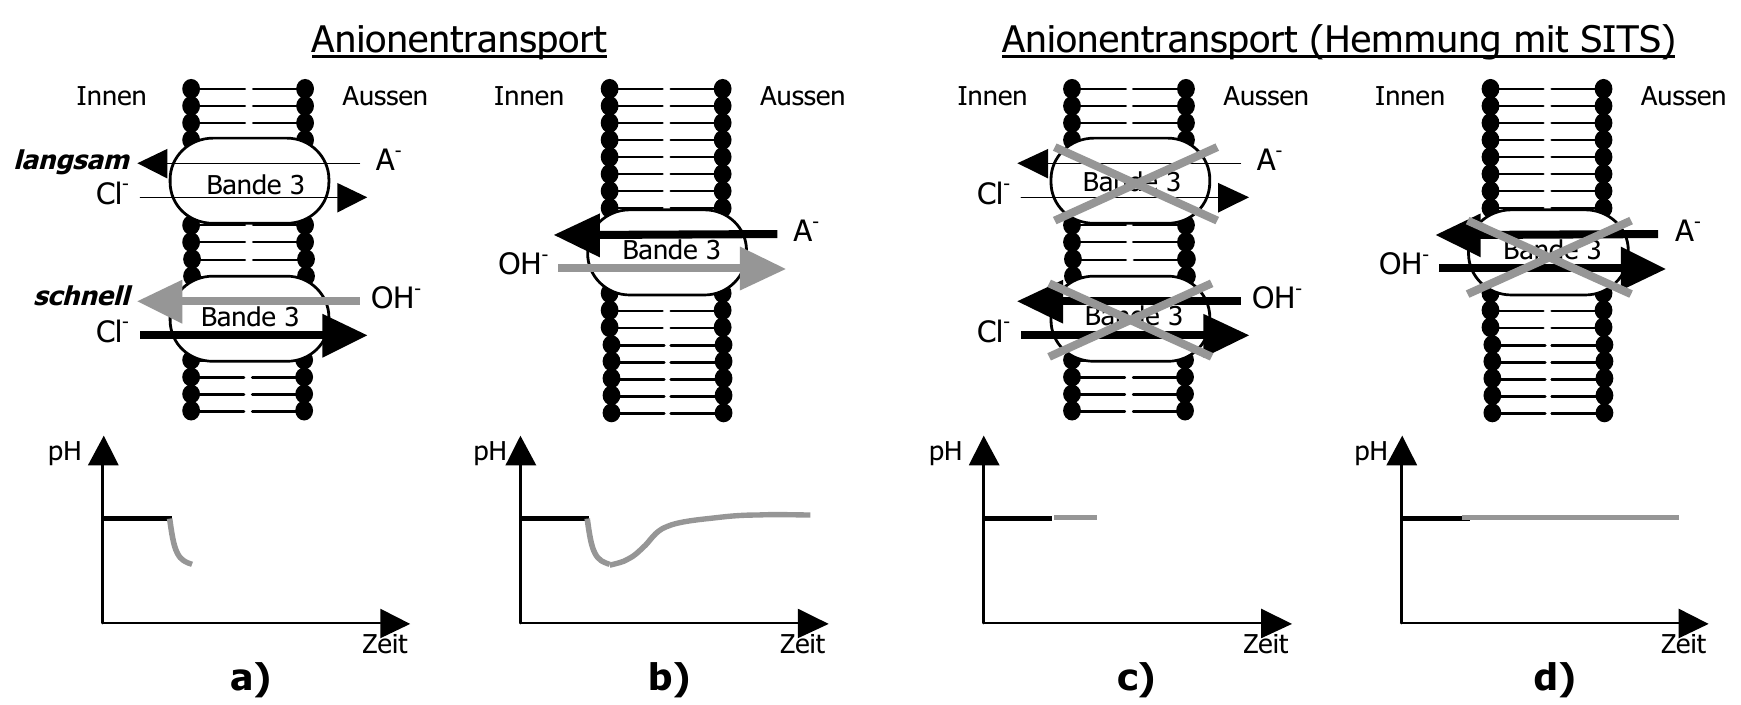
\includegraphics[width=0.9\textwidth]{img/th_transport_ph_ani}
	\caption{Effekt des Anionentransports auf extrazellulären pH aus \cite{skriptv6}}
	\label{fig:transport_ph_ani}
\end{figure}

\begin{figure}[h]
	\centering
	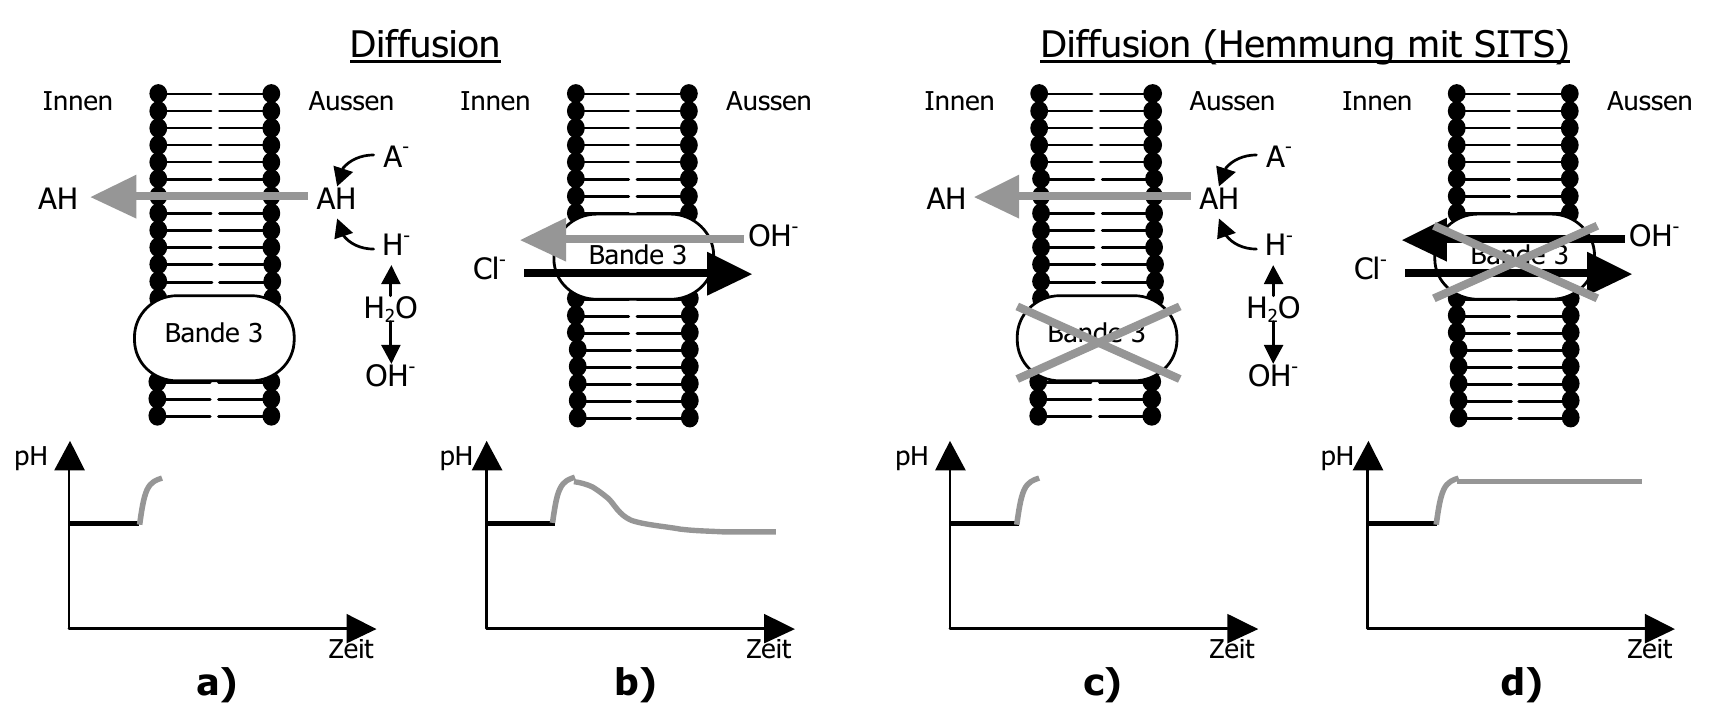
\includegraphics[width=0.9\textwidth]{img/th_transport_ph_diff}
	\caption{Effekt der Diffusion auf extrazellulären pH aus \cite{skriptv6}}
	\label{fig:transport_ph_diff}
\end{figure}

Im Falle des Anionentransports einer Säure stellt sich ein Gleichgewicht
basierend auf zwei Mechanismen ein. Sofort nach Zugabe der Säure zu den
Erythrozyten werden durch das Bande-3 Protein intrazelluläre \ce{Cl-} Anionen
gegen extrazelluläre \ce{OH-} Anionen ausgetauscht, was zu einer Erniedrigung
des extrazellulären pH Wertes führt (Abbildung \ref{fig:transport_ph_ani}, a)).
Im Anschluss wird durch den langsamer verlaufenden Austausch von Säure-Anionen
gegen \ce{OH-} Anionen der pH wieder ansteigen und sich stabilisieren
(Abbildung \ref{fig:transport_ph_ani}, b)).

Wird das Bande-3 Protein gehemmt, findet keiner der beiden Vorgänge statt, und
der pH bleibt konstant (Abbildung \ref{fig:transport_ph_ani}, c), d)).

Im Gegensatz dazu wandert im Falle der Diffusion die freie Säure in das
Zellinnere, was zu einem Transport von \ce{H+} (aus der Eigenprotonierung von
Wasser) ins Zellinnere führt. Dadurch steigt der extrazelluläre pH an
(Abbildung \ref{fig:transport_ph_diff} a)). Im Anschluss erfolgt durch das
Bande-3 Protein ein Austausch von \ce{Cl-} und \ce{OH-} statt, was dazu führt
dass sich der pH wieder senkt (Abbildung \ref{fig:transport_ph_diff}, b)).

Wird das Bande-3 Protein durch SITS deaktiviert, findet der zweite Austausch
nicht statt, und der pH verbleibt auf erhöhtem Niveau (Abbildung
\ref{fig:transport_ph_diff}, c), d)).

\subsection{Effekt auf Hämolyse}

\begin{figure}[h]
	\centering
	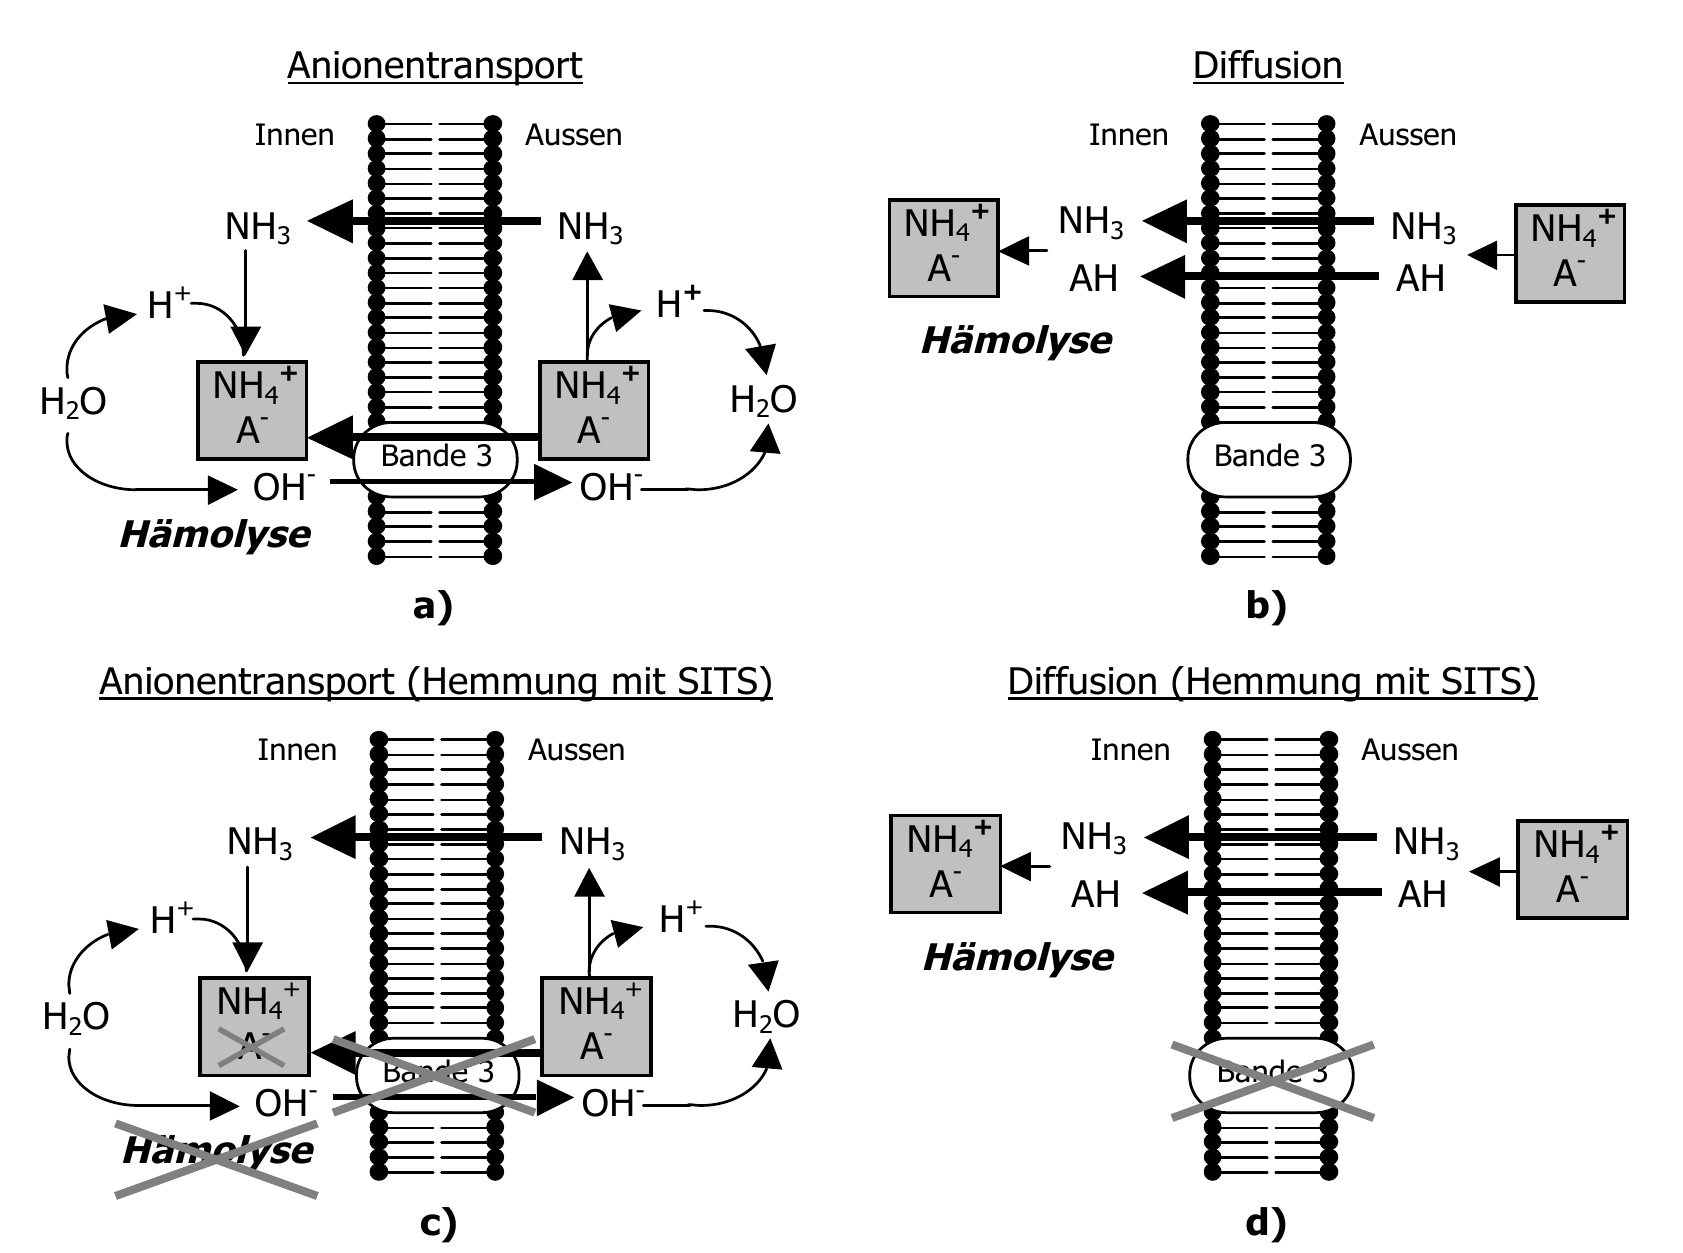
\includegraphics[width=0.9\textwidth]{img/th_transport_haem}
	\caption{Effekt des Transportes auf Hämolyse aus \cite{skriptv6}}
	\label{fig:transport_haem}
\end{figure}

Hämolyse der Zelle findet statt, falls ein Netto-Transport von \ce{NH3} in das
Zellinnere stattfindet. Dies geschieht, falls eine Säure via Anionentransport
(Abbildung \ref{fig:transport_haem} a)) oder Diffusion (Abbildung
\ref{fig:transport_haem} b), d)) die Zelle betritt. Im Falle des
Anionentransports - der durch SITS gehemmt wird - kommt es damit im gehemmten
Fall nicht zur Hämolyse (Abbildung \ref{fig:transport_haem} c)).

\section{Vorgehen}

Aus bereitgestellten Blutkonserven wurden von \SI{5}{ml} Blut durch zweifache
Zentrifugierung bei \SI{1000}{g} die Erythrozyten getrennt, in \SI{20}{ml} PBS-Glucose
aufgenommen, und auf Eis gelagert.

Aus \SI{0.5}{\Molar} Lösungen von sowohl des Natrium- als auch des
Ammoniumsalzes von Ameisen-, Essig-, Glyoxyl-, Wein- und Zitronensäure wurden
isotonische Lösungen hergestellt, damit es zu keiner Hämolyse durch Osmose
kommen kann.

Für die Natriumsalz-Lösungen wurde die Veränderung des pH bei Zugabe zu
Erythrozyten gemessen, jeweils eine Messreihe ohne, und eine Messreihe mit
Zugabe von SITS. Für die Ammoniak-Lösungen wurde im Photometer die Absorption
bei \SI{610}{nm} bei Zugabe zu Erythrozyten gemessen, ebenfalls jeweils mit und
ohne Zugabe von SITS.

Um sicherzustellen, dass die Hämolyse ein Resultat des eindringenden \ce{NH3}
ist, wurde eine letzte Messung vorgenommen, in welcher die Natriumsalz-Lösung
einer Säure, die als Ammonium-Salz zur Hämolyse führte, zu Erythrozyten
gegeben wurde. Um zu bestätigen dass \ce{NH3} für die Hämolyse verantwortlich
ist, war zu erwarten dass die Natriumsalz-Lösung zu keiner Hämolyse führte.

\chapter{Berechnungen}

Zwecks Verhinderung der Hämolyse durch Osmose wurden die bereitgestellten
Lösungen des Natrium- und Ammonium-Salzes von organischen Säuren auf
isotonische Konzentrationen von \SI{300}{mOsm} verdünnt.

Die Osmolarität einer Lösung lässt sich abschätzen durch Anzahl gelöster Ionen
je Volumen. Eine \SI{1}{\Molar} Lösung einer einprotonigen Säure bei \si{pH}
7.4 hat somit eine Osmolarität von ca \SI{2}{Osm}, wobei eines der Ionen das
Säure-Anion, das andere ihr Kation, ist. Damit folgen für die die
vorbereiteten \SI{0.5}{\Molar} Lösungen folgende Verdünnungsfaktoren für eine
isotonische Lösung mit \SI{300}{mOsm}.
\\

\begin{tabu}{lclc}
	\toprule
	Säure & Wertigkeit & Osmolarität & Verdünnungsfaktor \\
	\midrule
	\SI{0.5}{\Molar} Ameisensäure  & 1 & \SI{1}{Osm}   & 30\% \\
	\SI{0.5}{\Molar} Essigsäure    & 1 & \SI{1}{Osm}   & 30\% \\
	\SI{0.5}{\Molar} Glyoxylsäure  & 1 & \SI{1}{Osm}   & 30\% \\
	\SI{0.5}{\Molar} Weinsäure     & 2 & \SI{1.5}{Osm} & 20\% \\
	\SI{0.5}{\Molar} Zitronensäure & 3 & \SI{2}{Osm}   & 15\% \\
	\bottomrule
\end{tabu}

\chapter{Resultate}

\section{Diskussion}

In den folgenden Graphen der pH Messungen kennzeichnet die senkrechte rote
Linie jeweils den Zeitpunkt der Zugabe der Erythrozyten zu den Lösungen der
organischen Säure. In den Graphen der Absorptions Messung kennzeichnet - falls
sinnvoll - die senkrechte graue Linie die Halbwertszeit.

\subsection{Ameisensäure}

\begin{figure}
	\centering
	\begin{subfigure}{.5\textwidth}
		\centering
		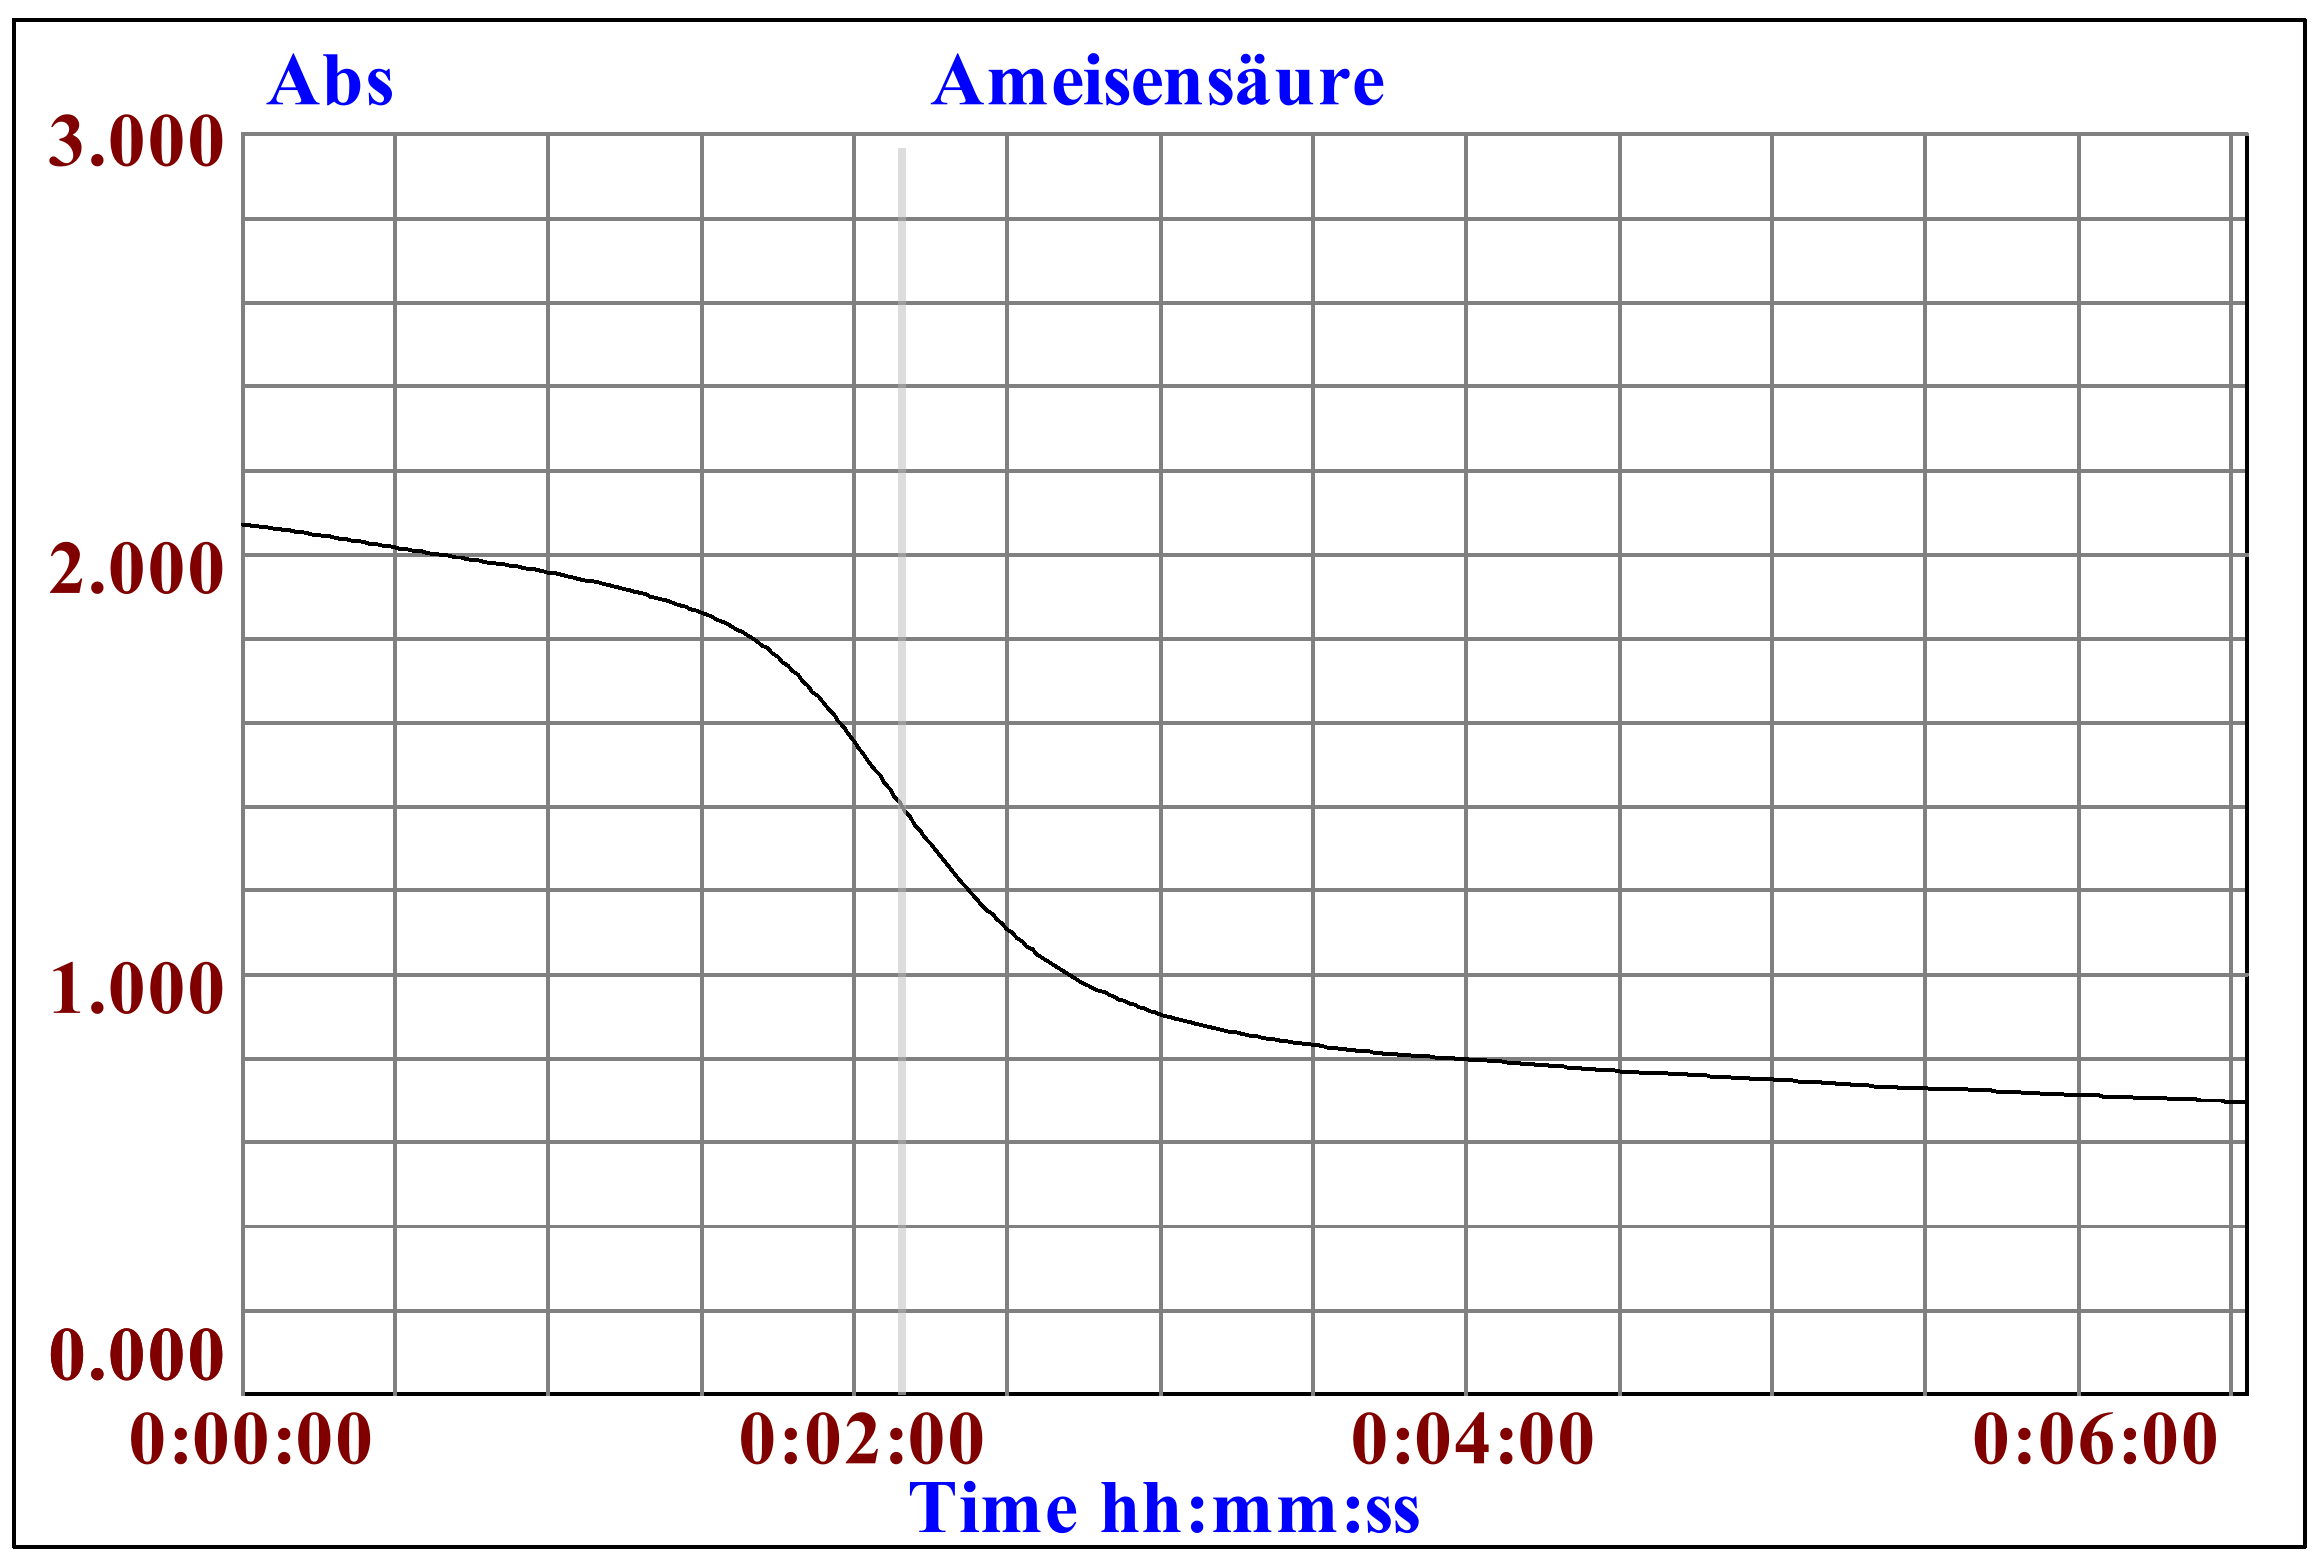
\includegraphics[width=\linewidth]{img/haem_ameisen.png}
		\caption{Ameisensäure}
	\end{subfigure}%
	\begin{subfigure}{.5\textwidth}
		\centering
		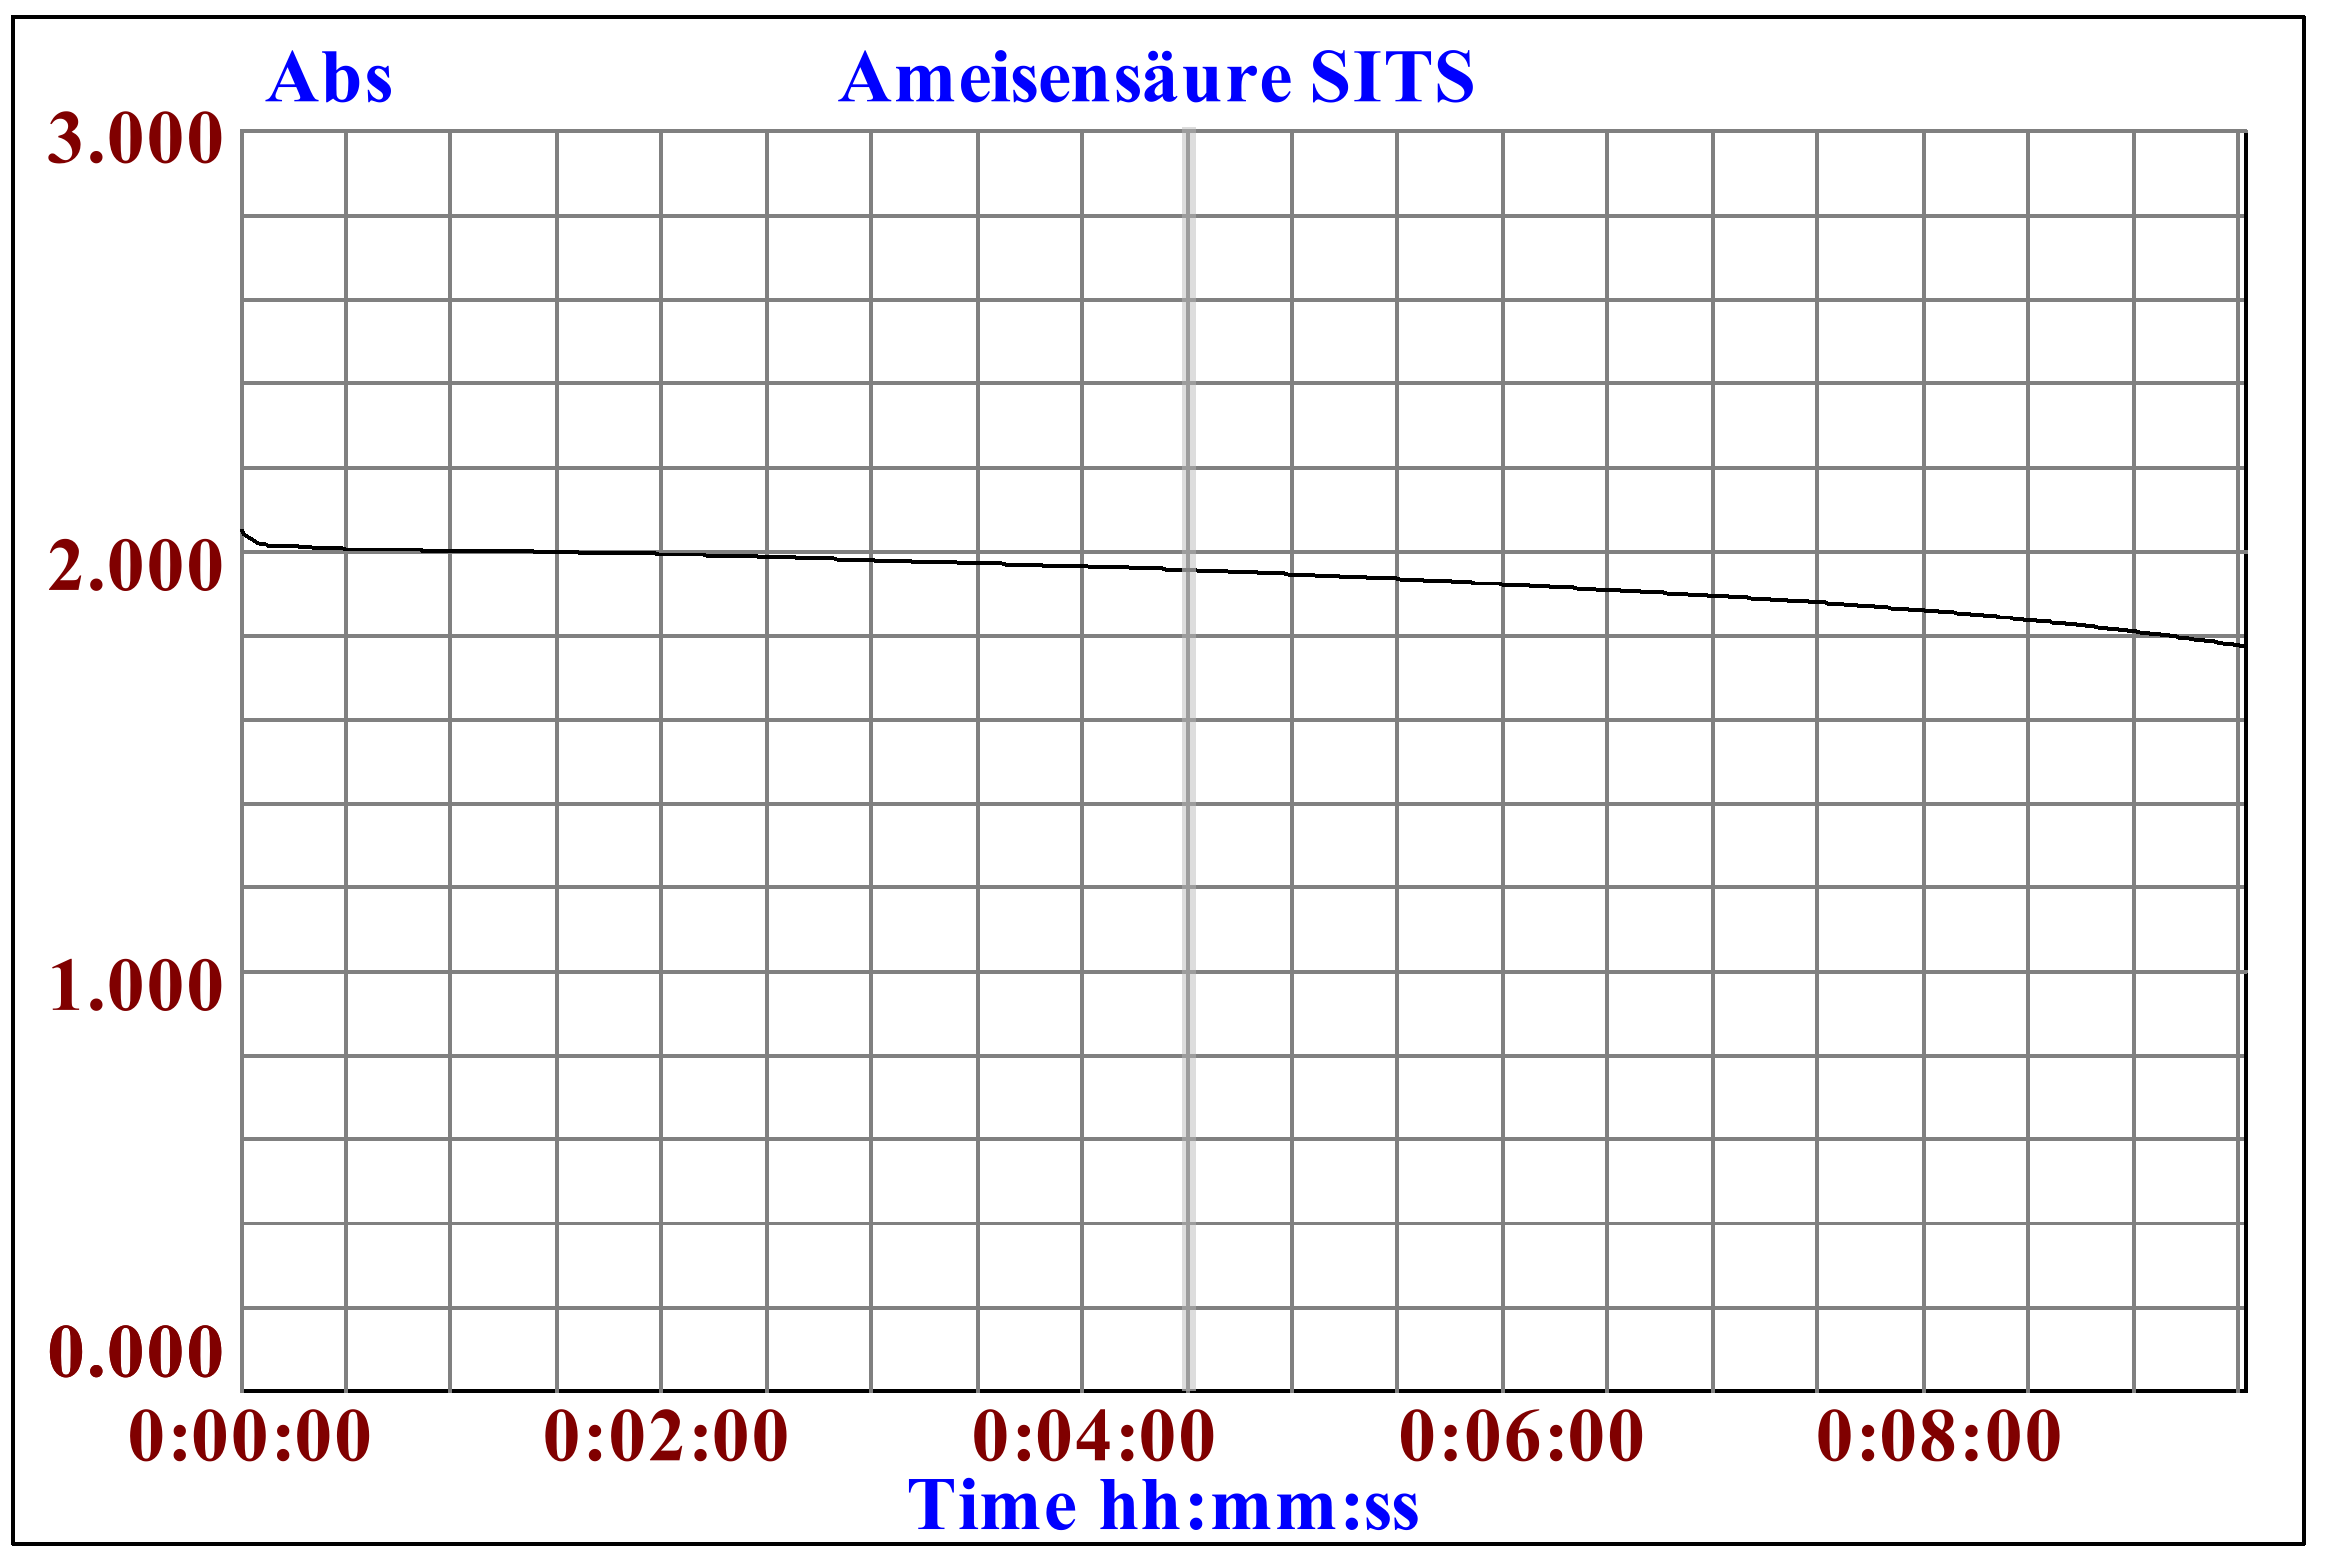
\includegraphics[width=\linewidth]{img/haem_ameisen_sits.png}
		\caption{Ameisensäure \& SITS}
	\end{subfigure}
	\caption{Absorption von Ameisensäure bei \SI{610}{nm}}
	\label{fig:haem_ameisen}
\end{figure}

\begin{figure}
	\centering
	\begin{subfigure}{.5\textwidth}
		\centering
		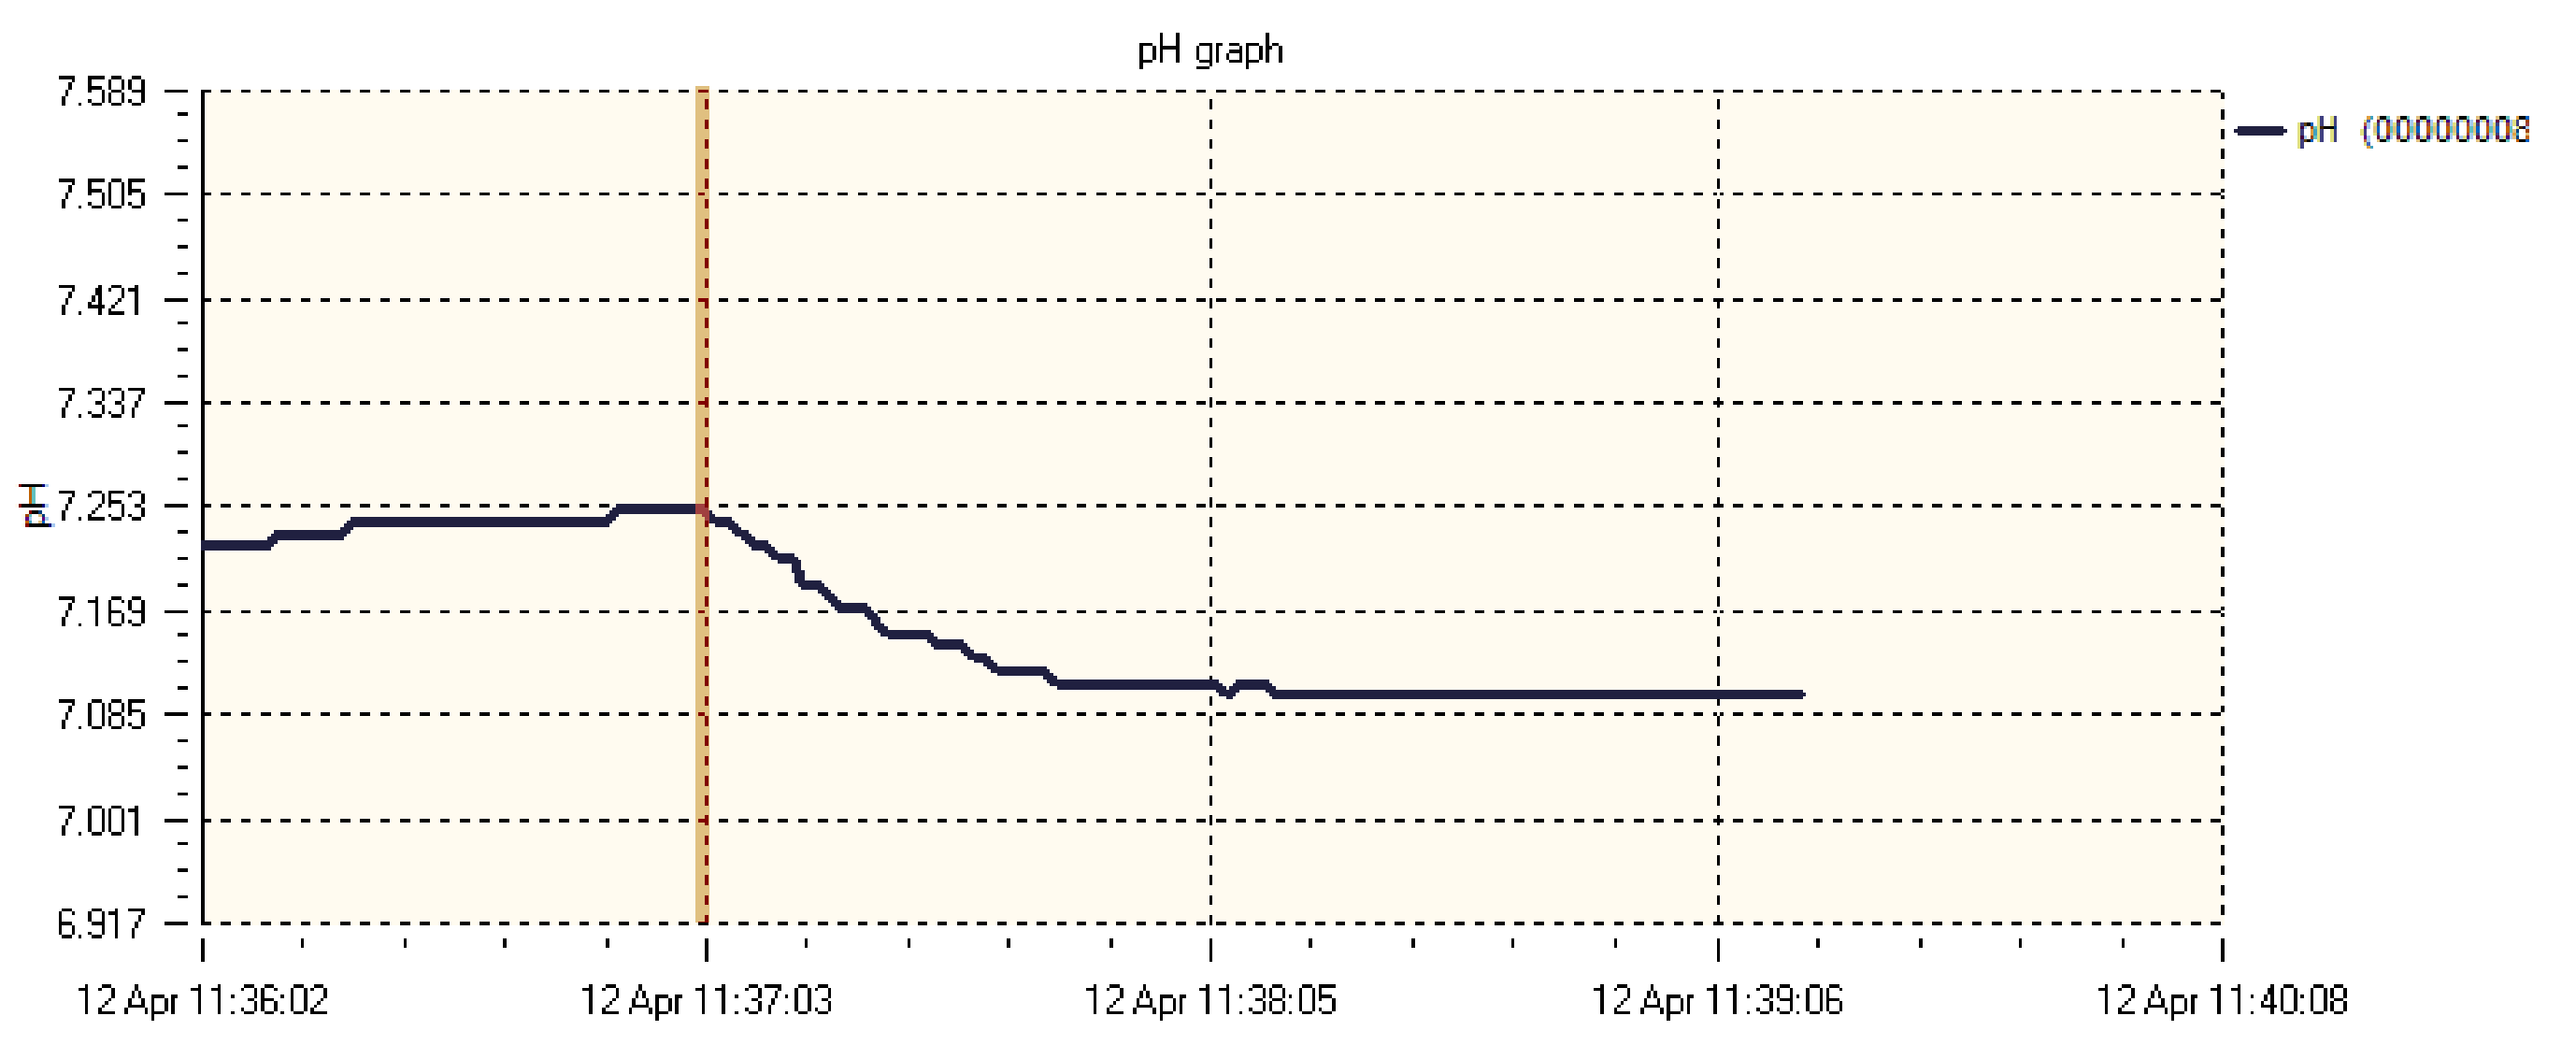
\includegraphics[width=\linewidth]{img/ph_ameisen.png}
		\caption{Ameisensäure}
	\end{subfigure}%
	\begin{subfigure}{.5\textwidth}
		\centering
		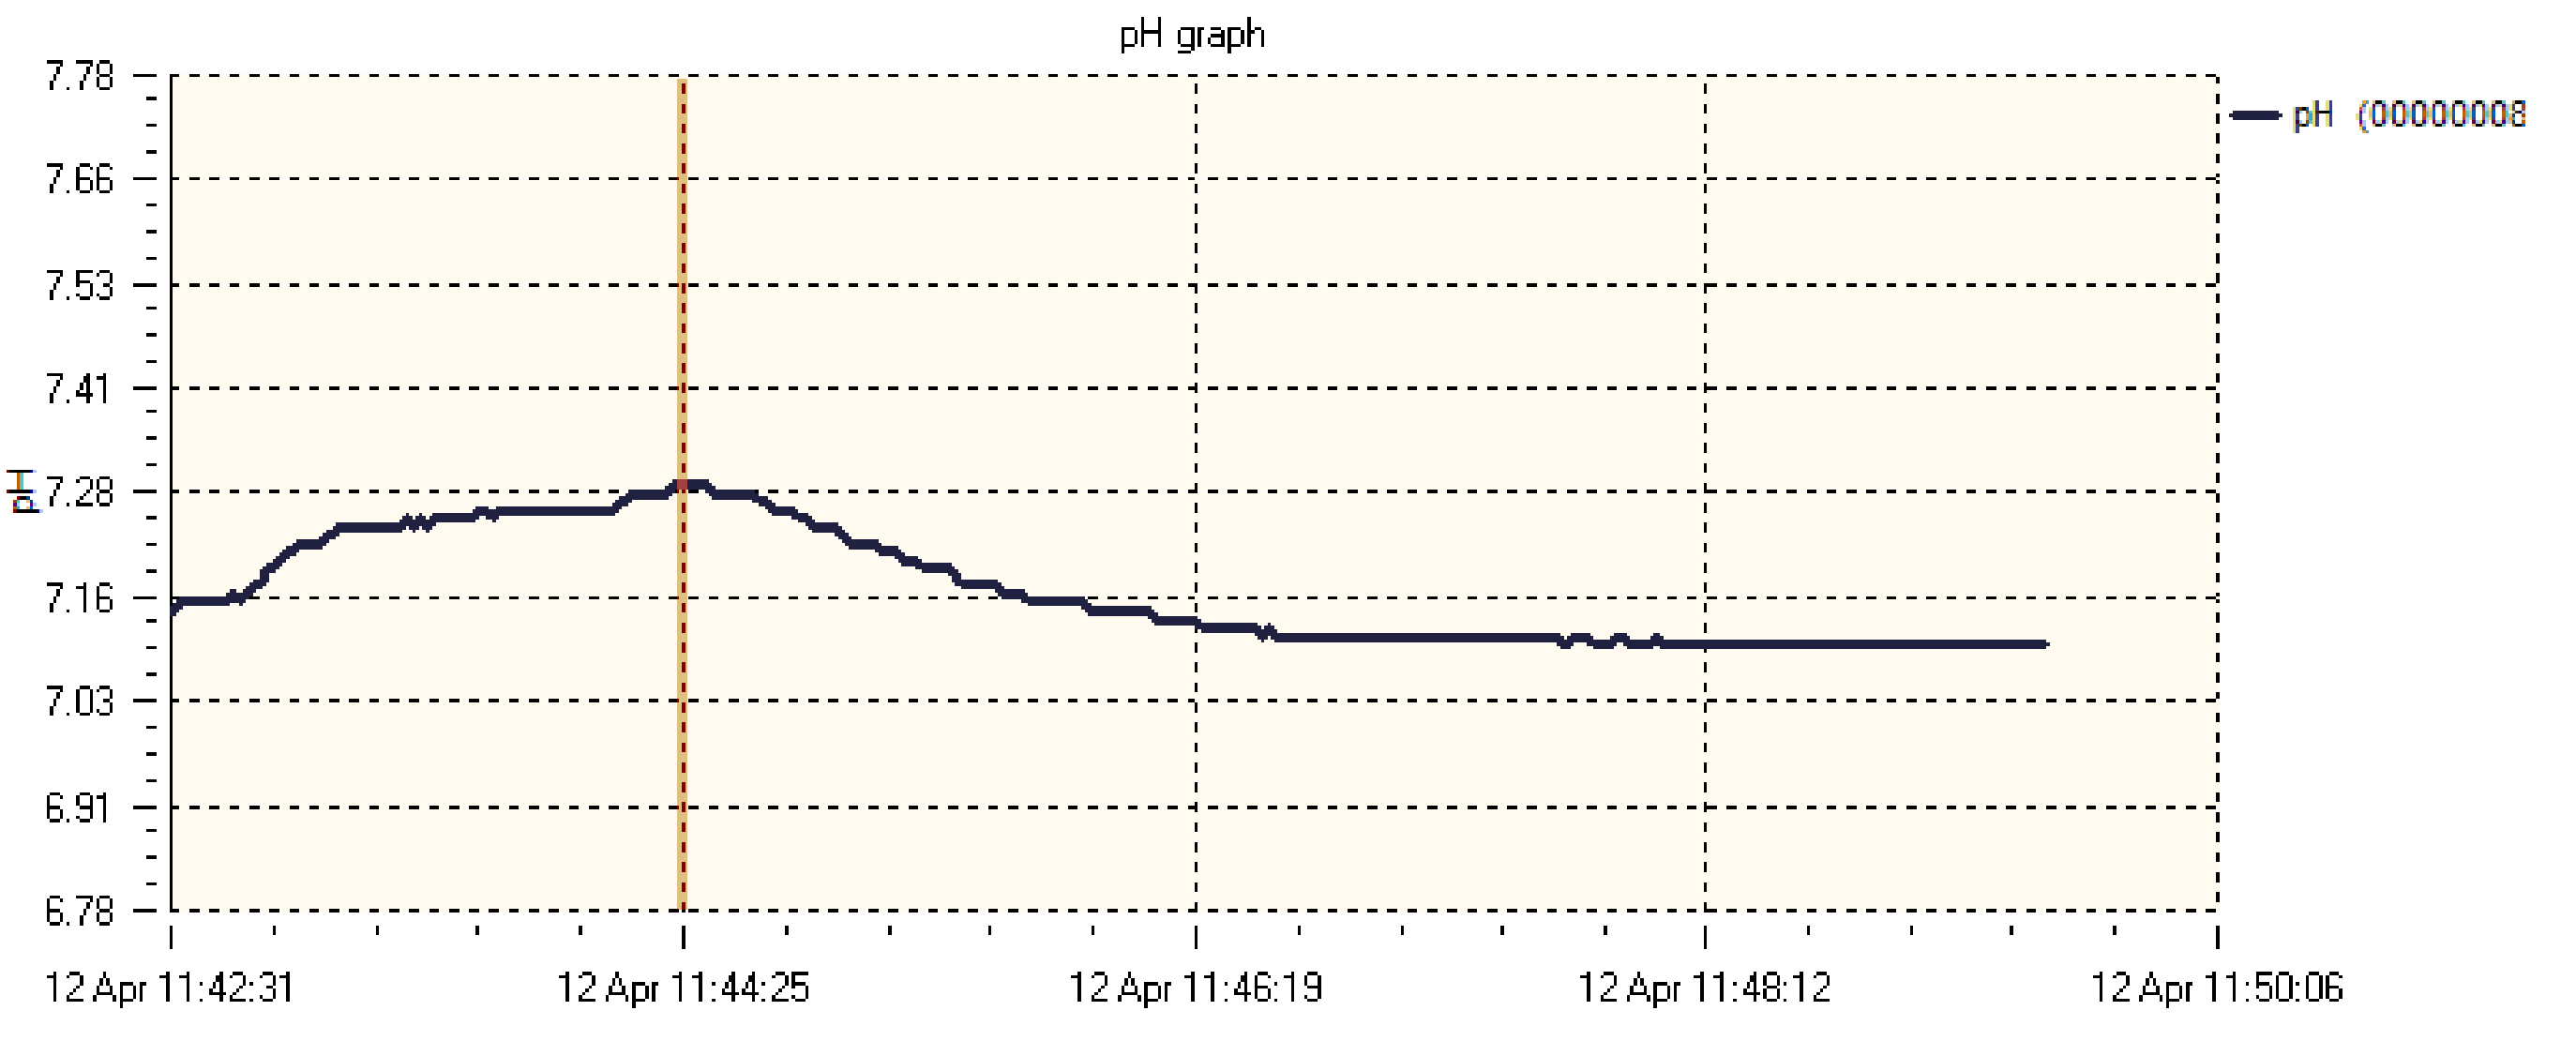
\includegraphics[width=\linewidth]{img/ph_ameisen_sits.png}
		\caption{Ameisensäure \& SITS}
	\end{subfigure}
	\caption{Extrazellulärer pH von Ameisensäure}
	\label{fig:ph_ameisen}
\end{figure}

In Abbildung \ref{fig:haem_ameisen} ist ersichtlich, dass es im Assay ohne SITS
zur Hämolyse kam, während im Assay mit SITS diese kaum stattfand. Dies
impliziert, dass die Ameisensäure via Bande-3 Protein durch die Membran
transportiert wird.

Dies lässt sich allerdings nicht mit der pH Messung der beiden Assays
bestätigen. Zwar sinkt der pH jenes Assays ohne SITS wie erwartet aufgrund des
Austausches von \ce{Cl-} und \ce{OH-} ab, aber der erwartete Ausgleich durch
Transport der Säure-Anionen via Bande-3 Protein bleibt aus.

\subsection{Essigsäure}

\begin{figure}
	\centering
	\begin{subfigure}{.5\textwidth}
		\centering
		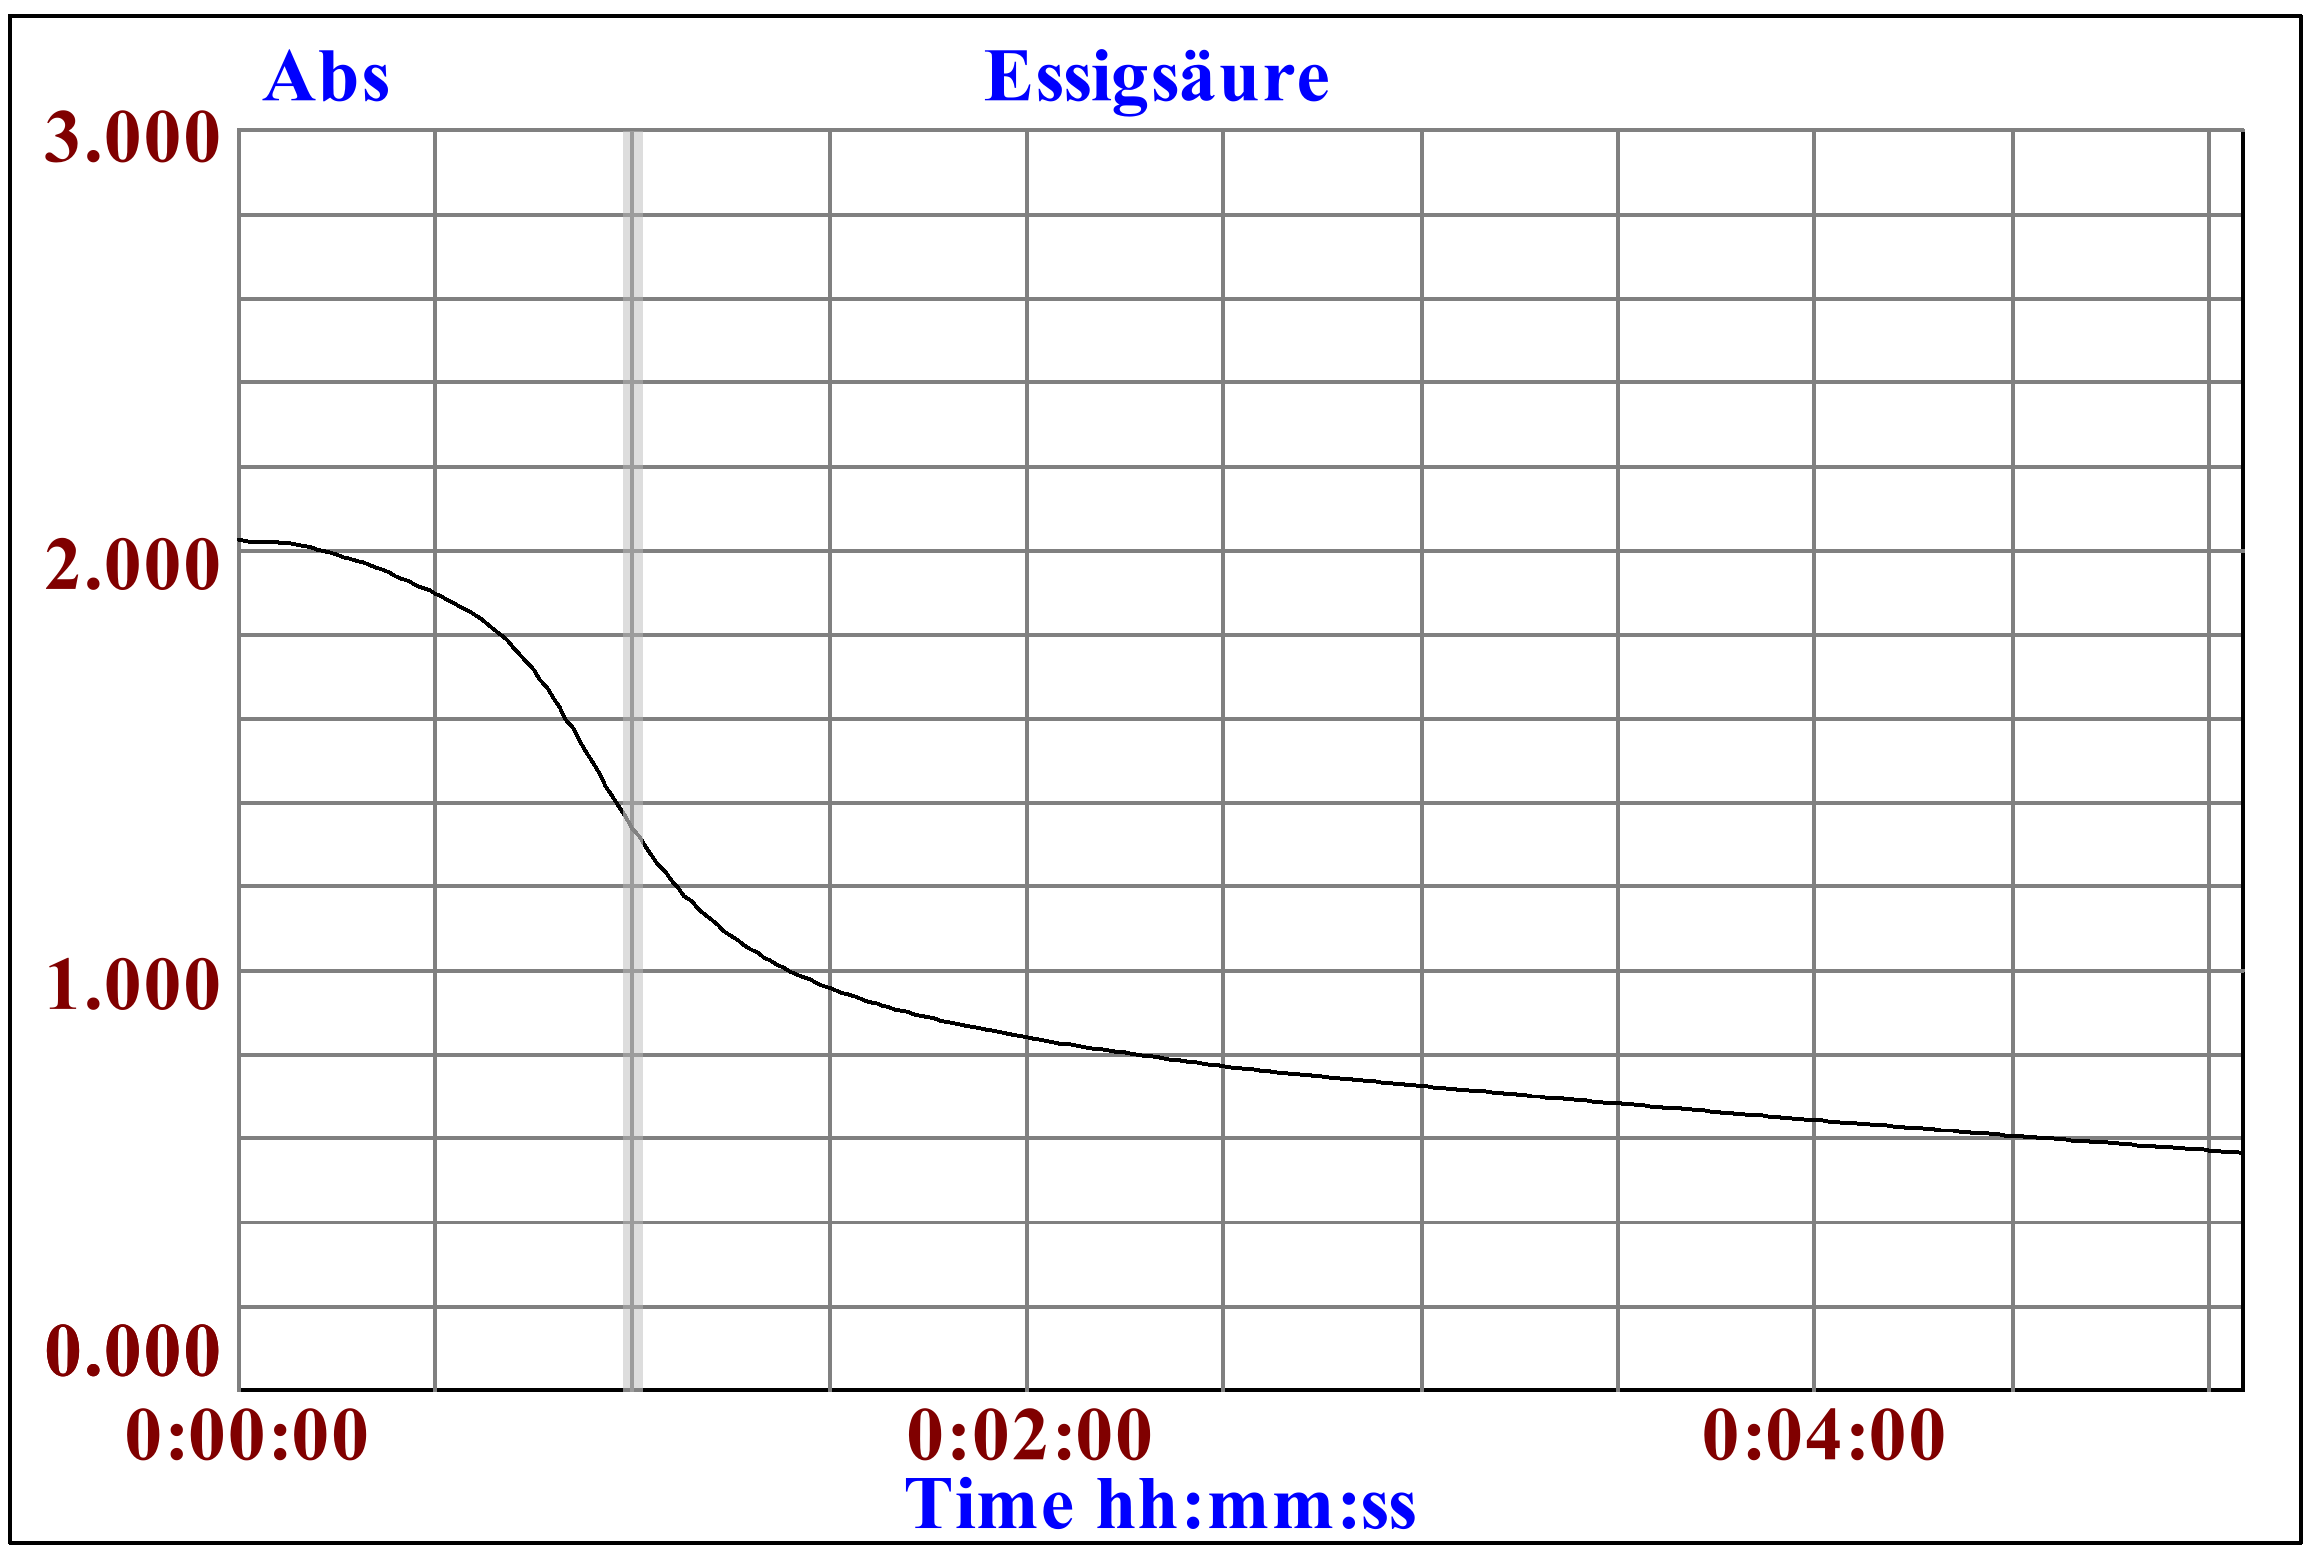
\includegraphics[width=\linewidth]{img/haem_essig.png}
		\caption{Essigsäure}
	\end{subfigure}%
	\begin{subfigure}{.5\textwidth}
		\centering
		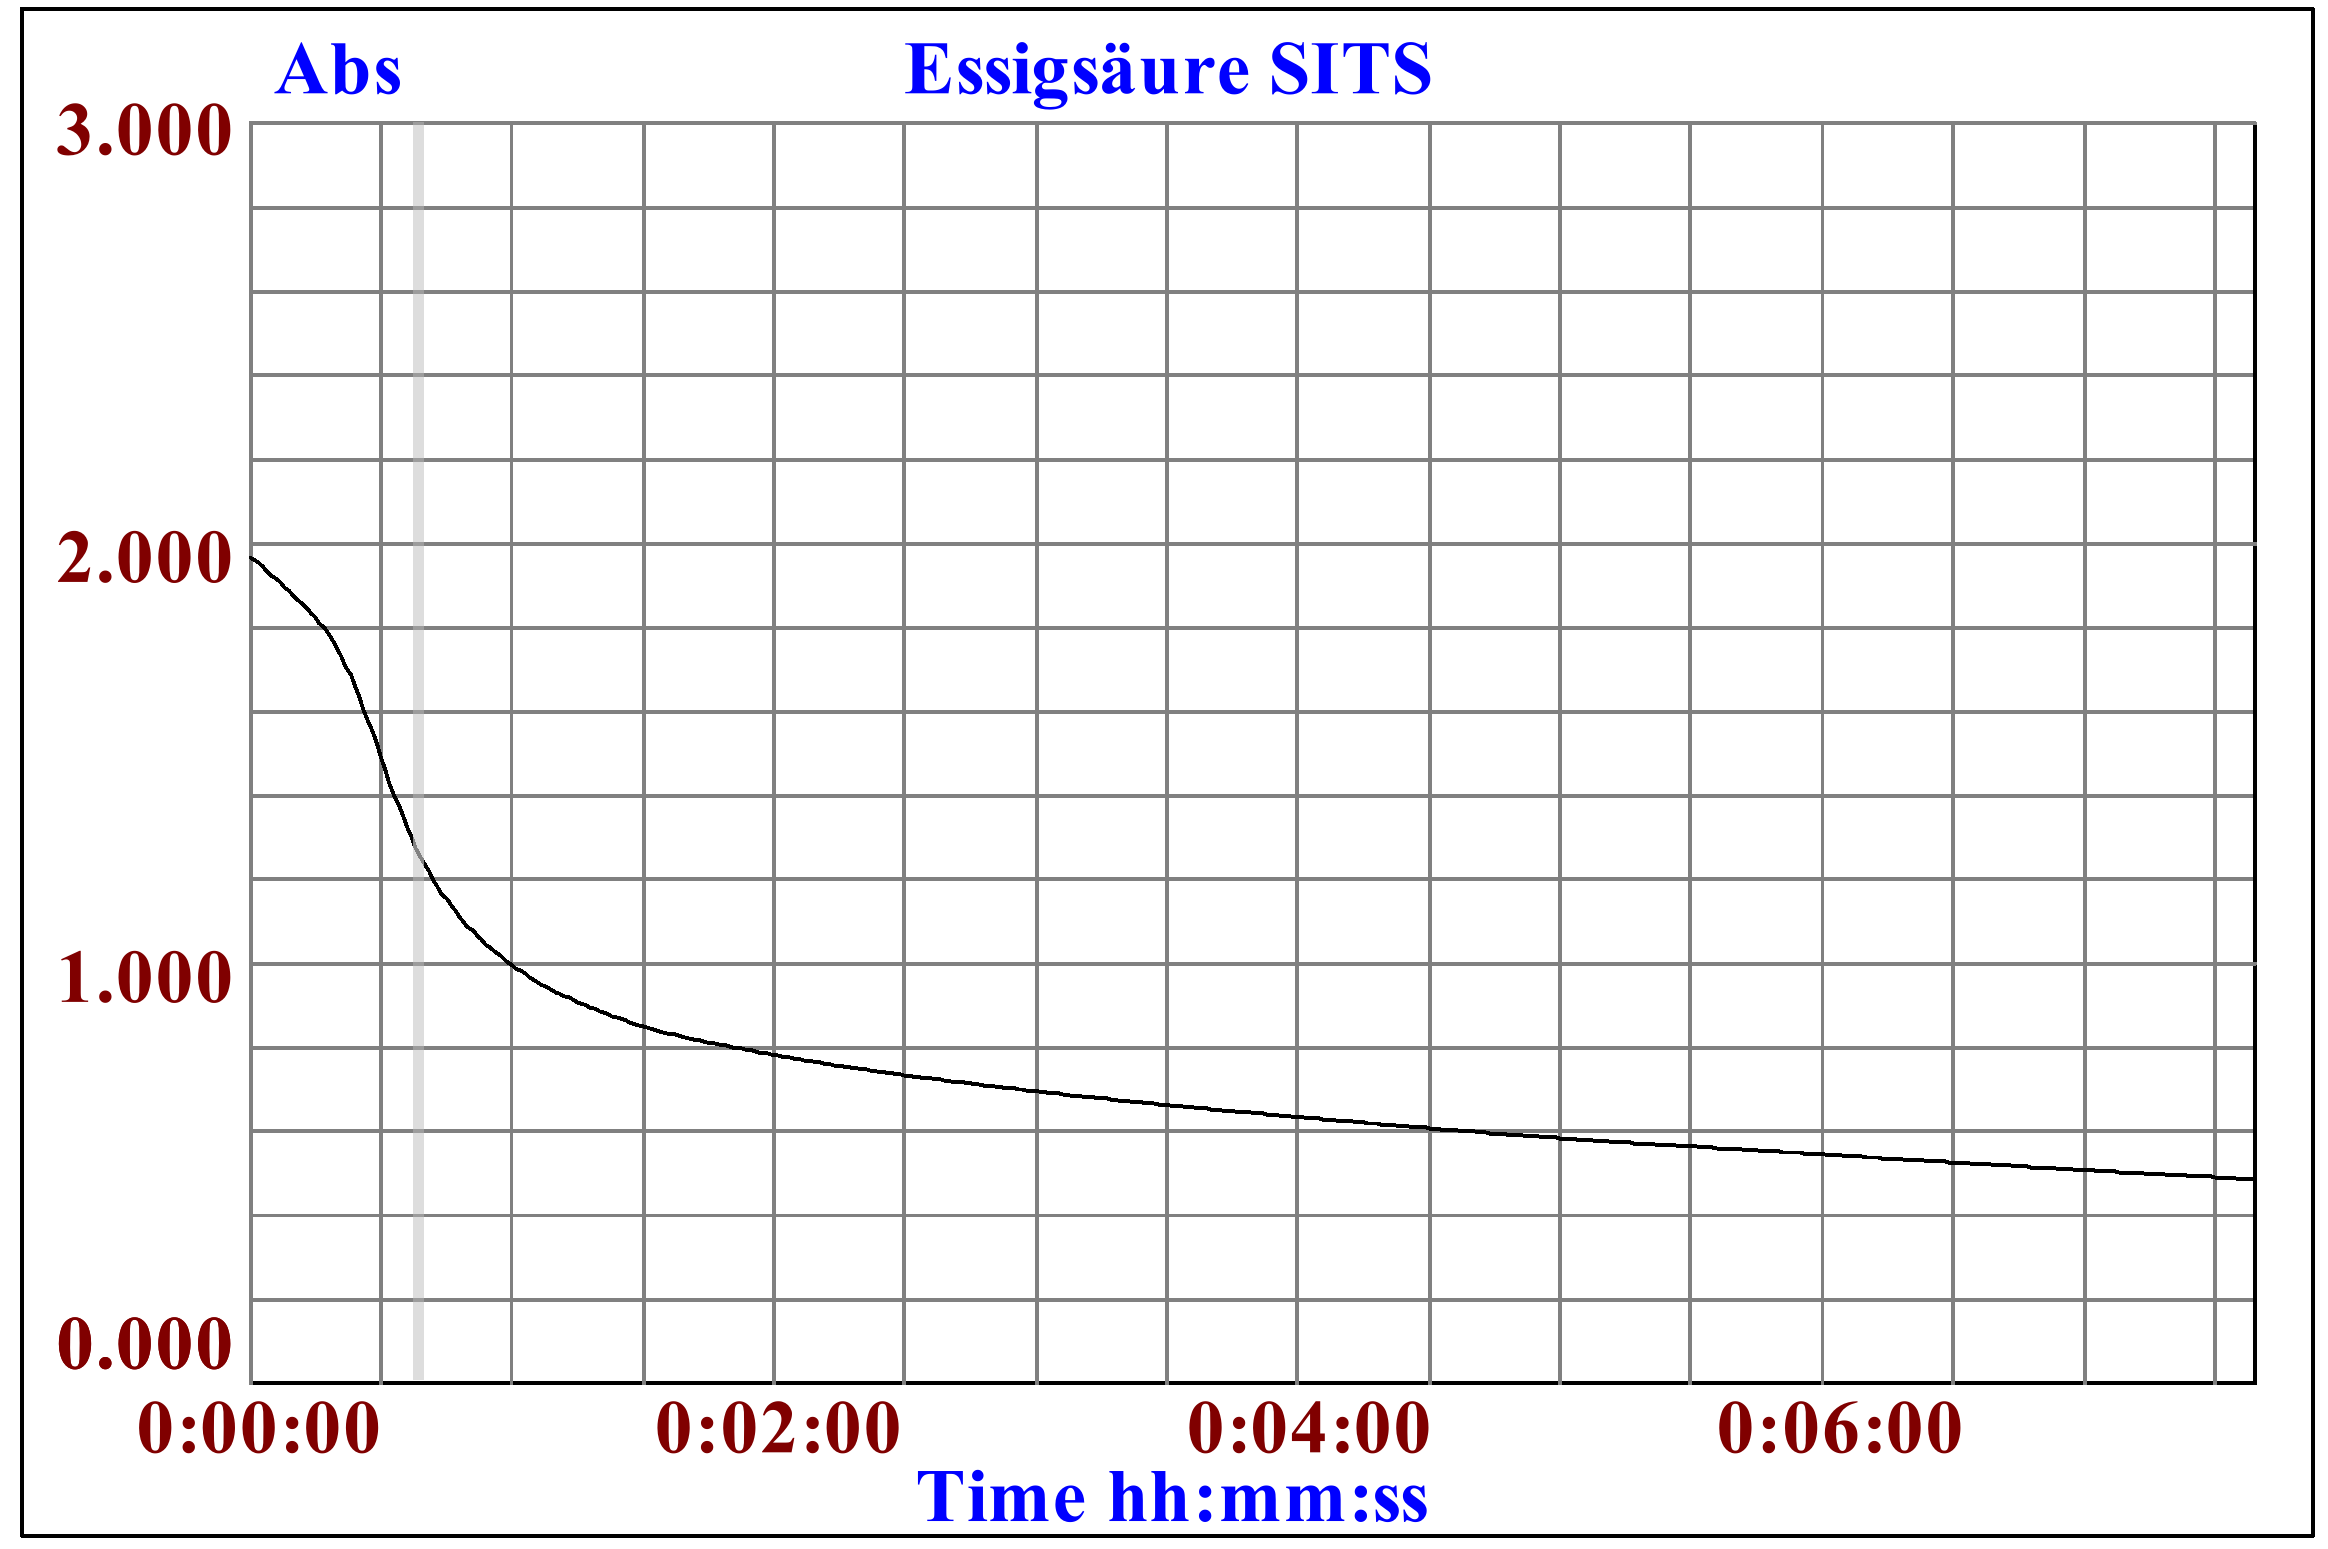
\includegraphics[width=\linewidth]{img/haem_essig_sits.png}
		\caption{Essigsäure \& SITS}
	\end{subfigure}
	\caption{Absorption von Essigsäure bei \SI{610}{nm}}
	\label{fig:haem_essig}
\end{figure}

\begin{figure}
	\centering
	\begin{subfigure}{.5\textwidth}
		\centering
		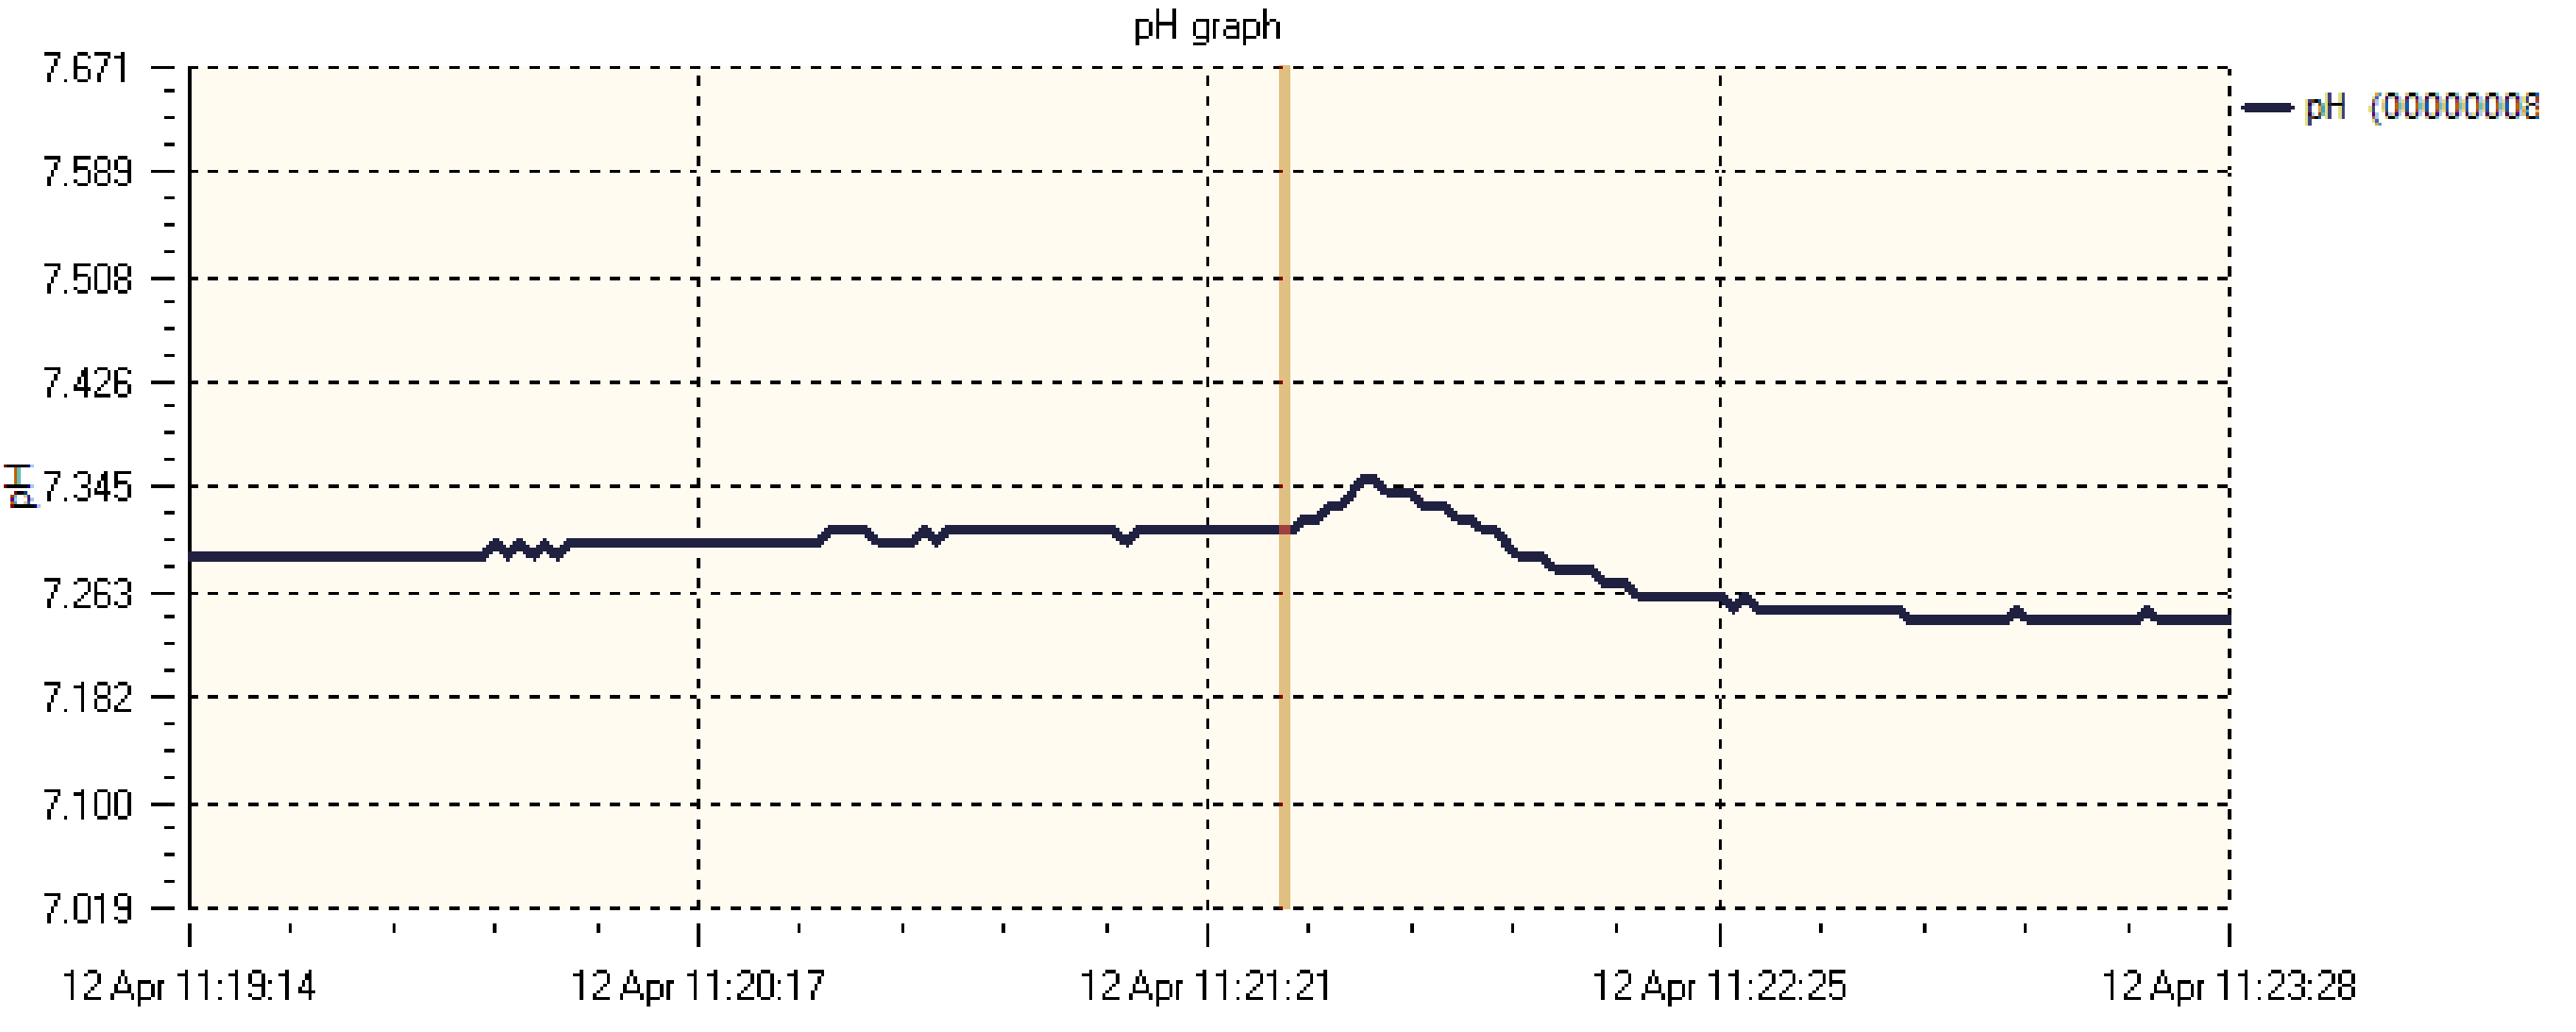
\includegraphics[width=\linewidth]{img/ph_essig.png}
		\caption{Essigsäure}
	\end{subfigure}%
	\begin{subfigure}{.5\textwidth}
		\centering
		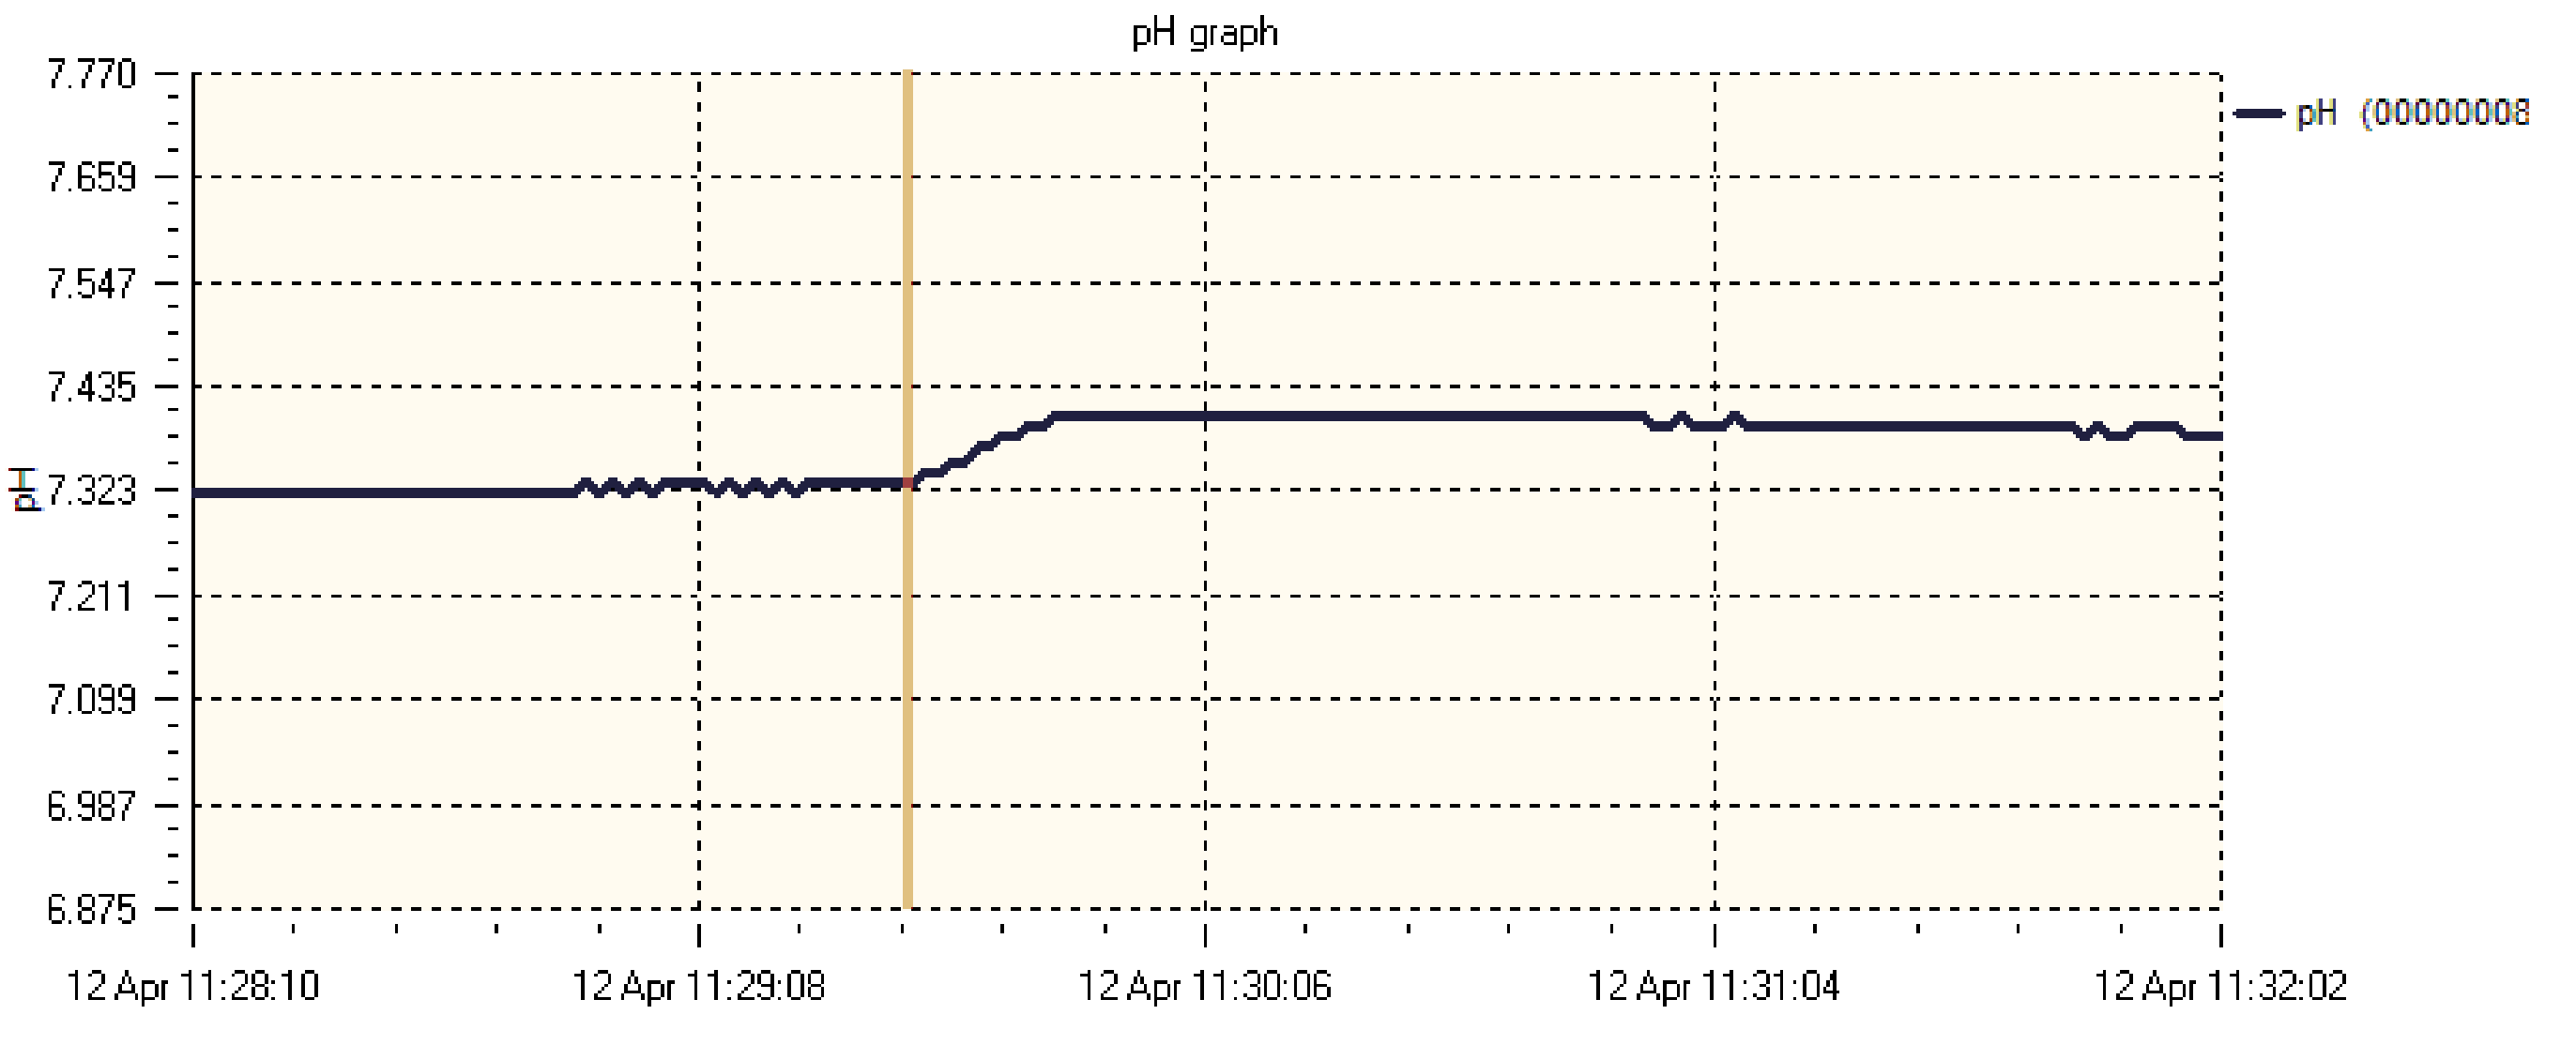
\includegraphics[width=\linewidth]{img/ph_essig_sits.png}
		\caption{Essigsäure \& SITS}
	\end{subfigure}
	\caption{Extrazellulärer pH von Essigsäure}
	\label{fig:ph_essig}
\end{figure}

Aus der Absorptionsmessung in Abbildung \ref{fig:haem_essig} ist ersichtlich,
dass es zur Hämolyse kam, egal ob SITS im System vorhanden war oder nicht. Dies
impliziert, dass Essigsäure die Zelle via Diffusion betritt.

Dies lässt sich mit der pH Messung in Abbildung \ref{fig:ph_essig} bestätigen,
in welcher sich der pH sowohl mit als auch ohne SITS so verhält wie erwartet.

\subsection{Glyoxylsäure}

\begin{figure}
	\centering
	\begin{subfigure}{.5\textwidth}
		\centering
		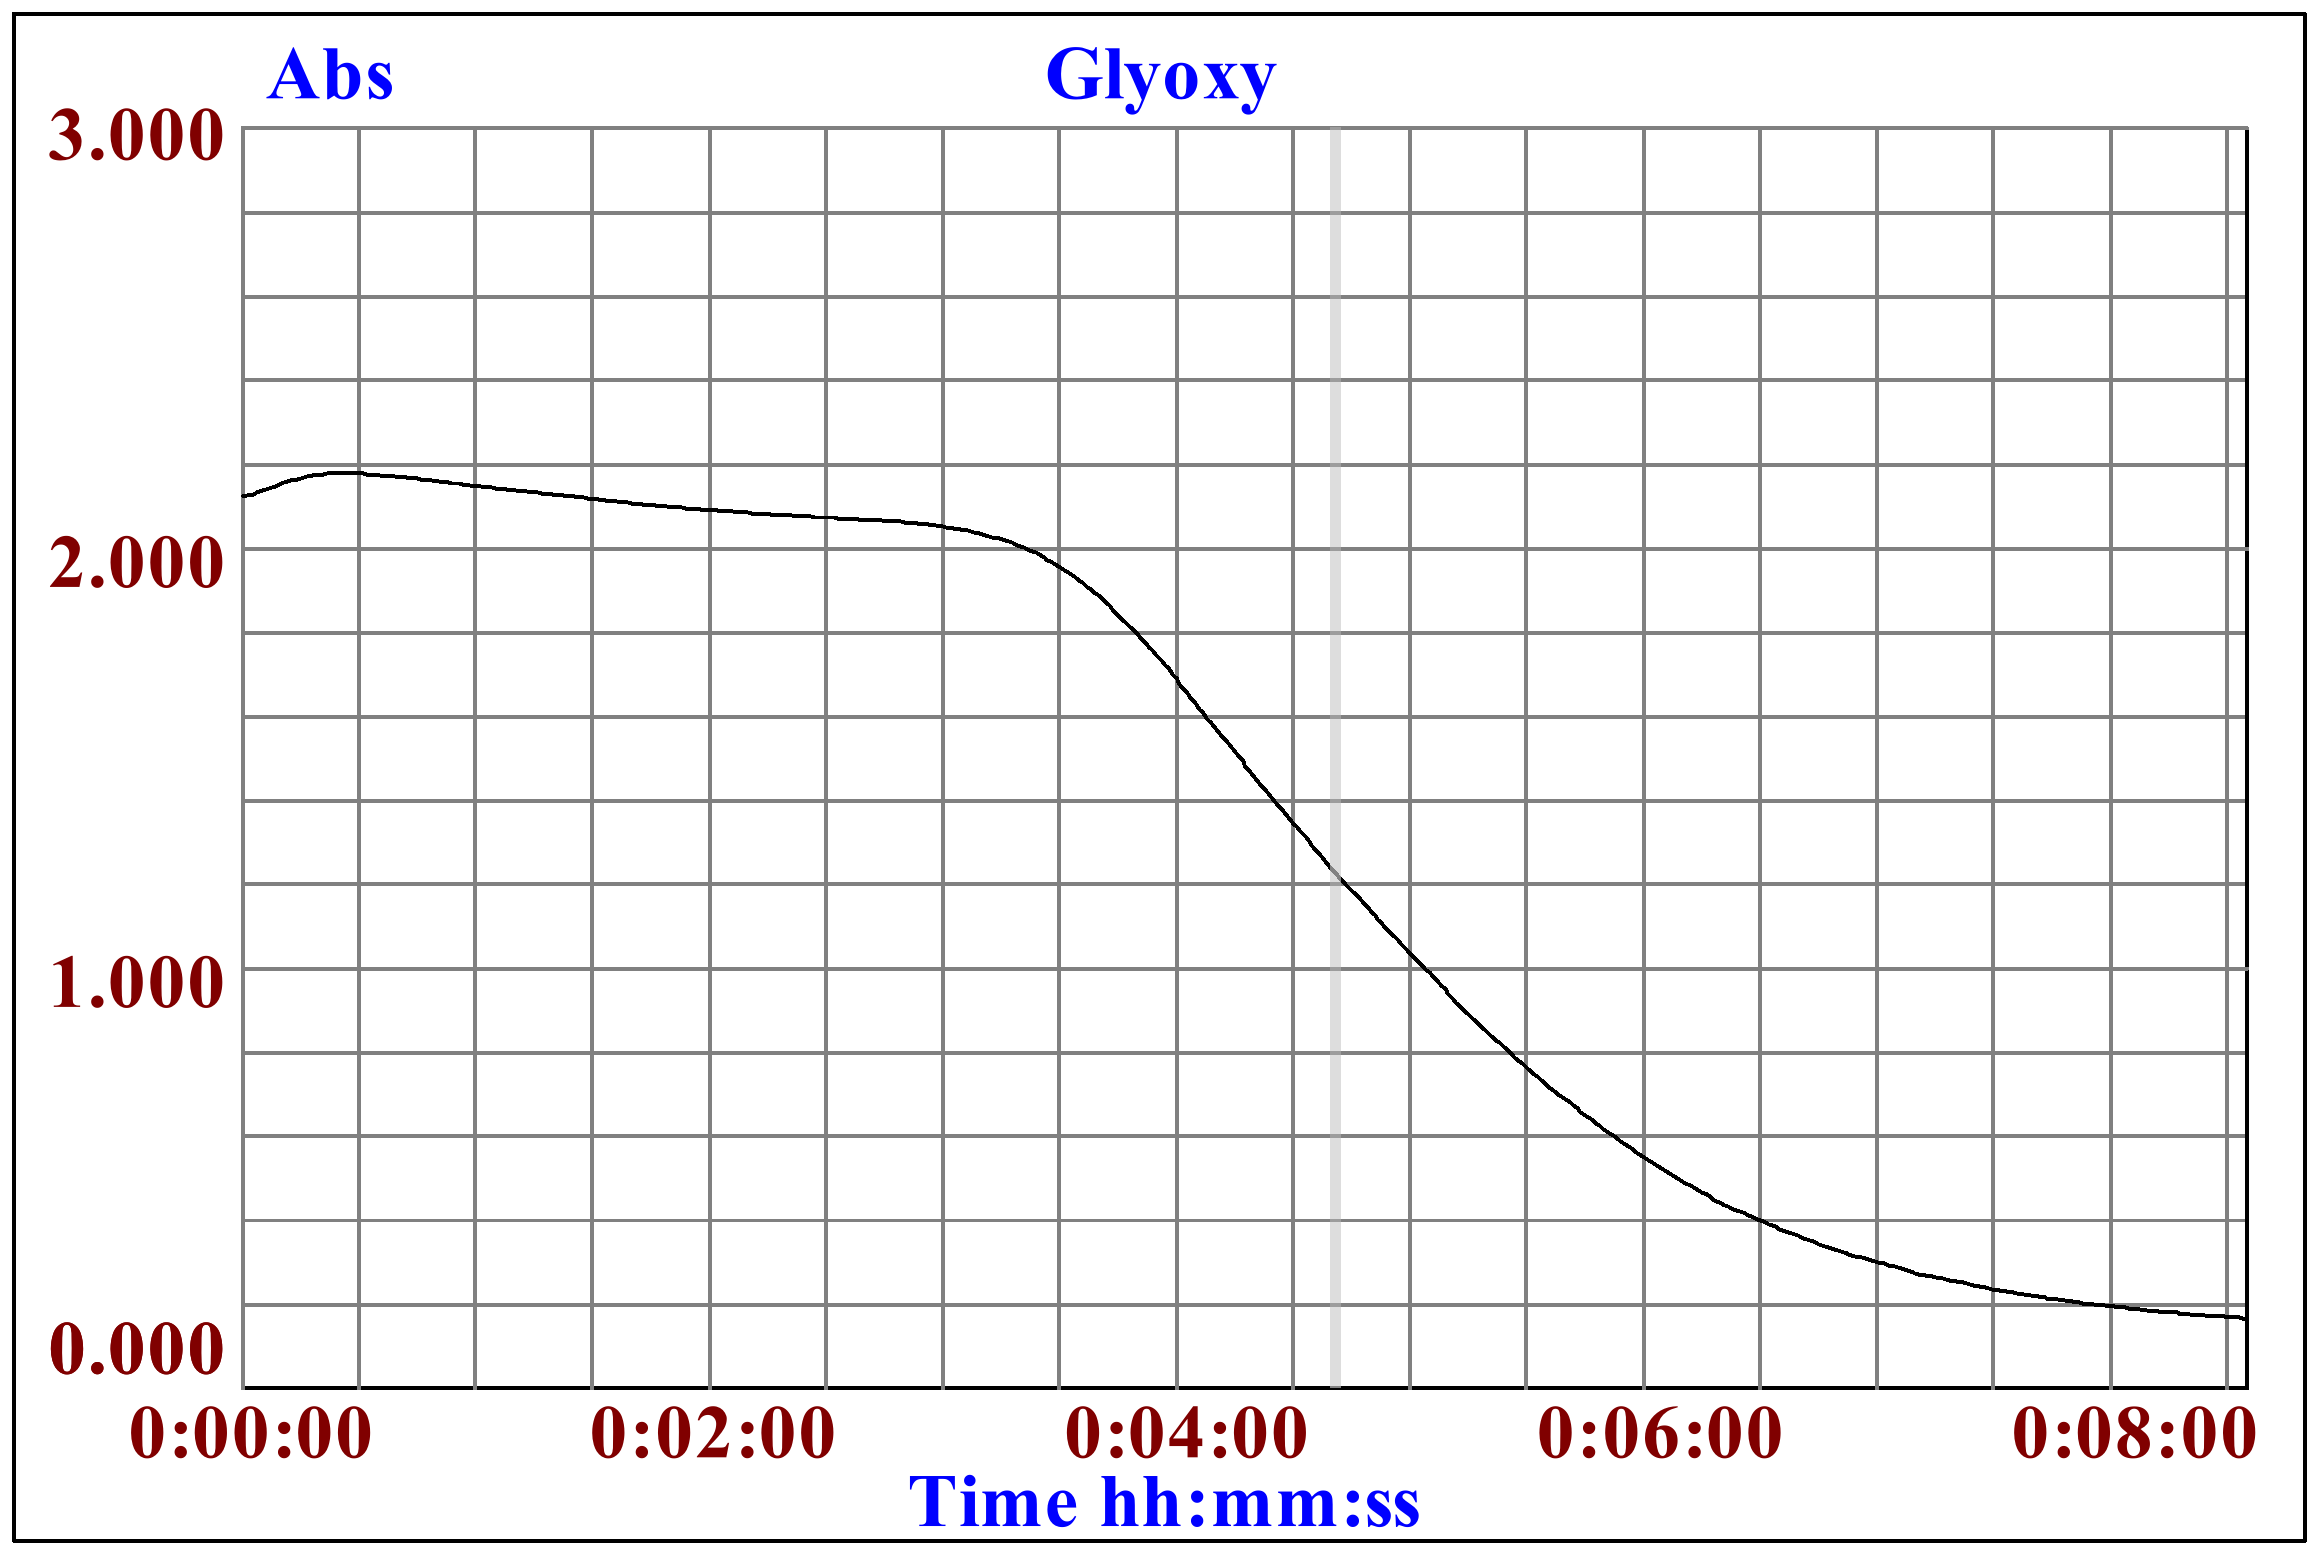
\includegraphics[width=\linewidth]{img/haem_glyoxy.png}
		\caption{Glyoxylsäure}
	\end{subfigure}%
	\begin{subfigure}{.5\textwidth}
		\centering
		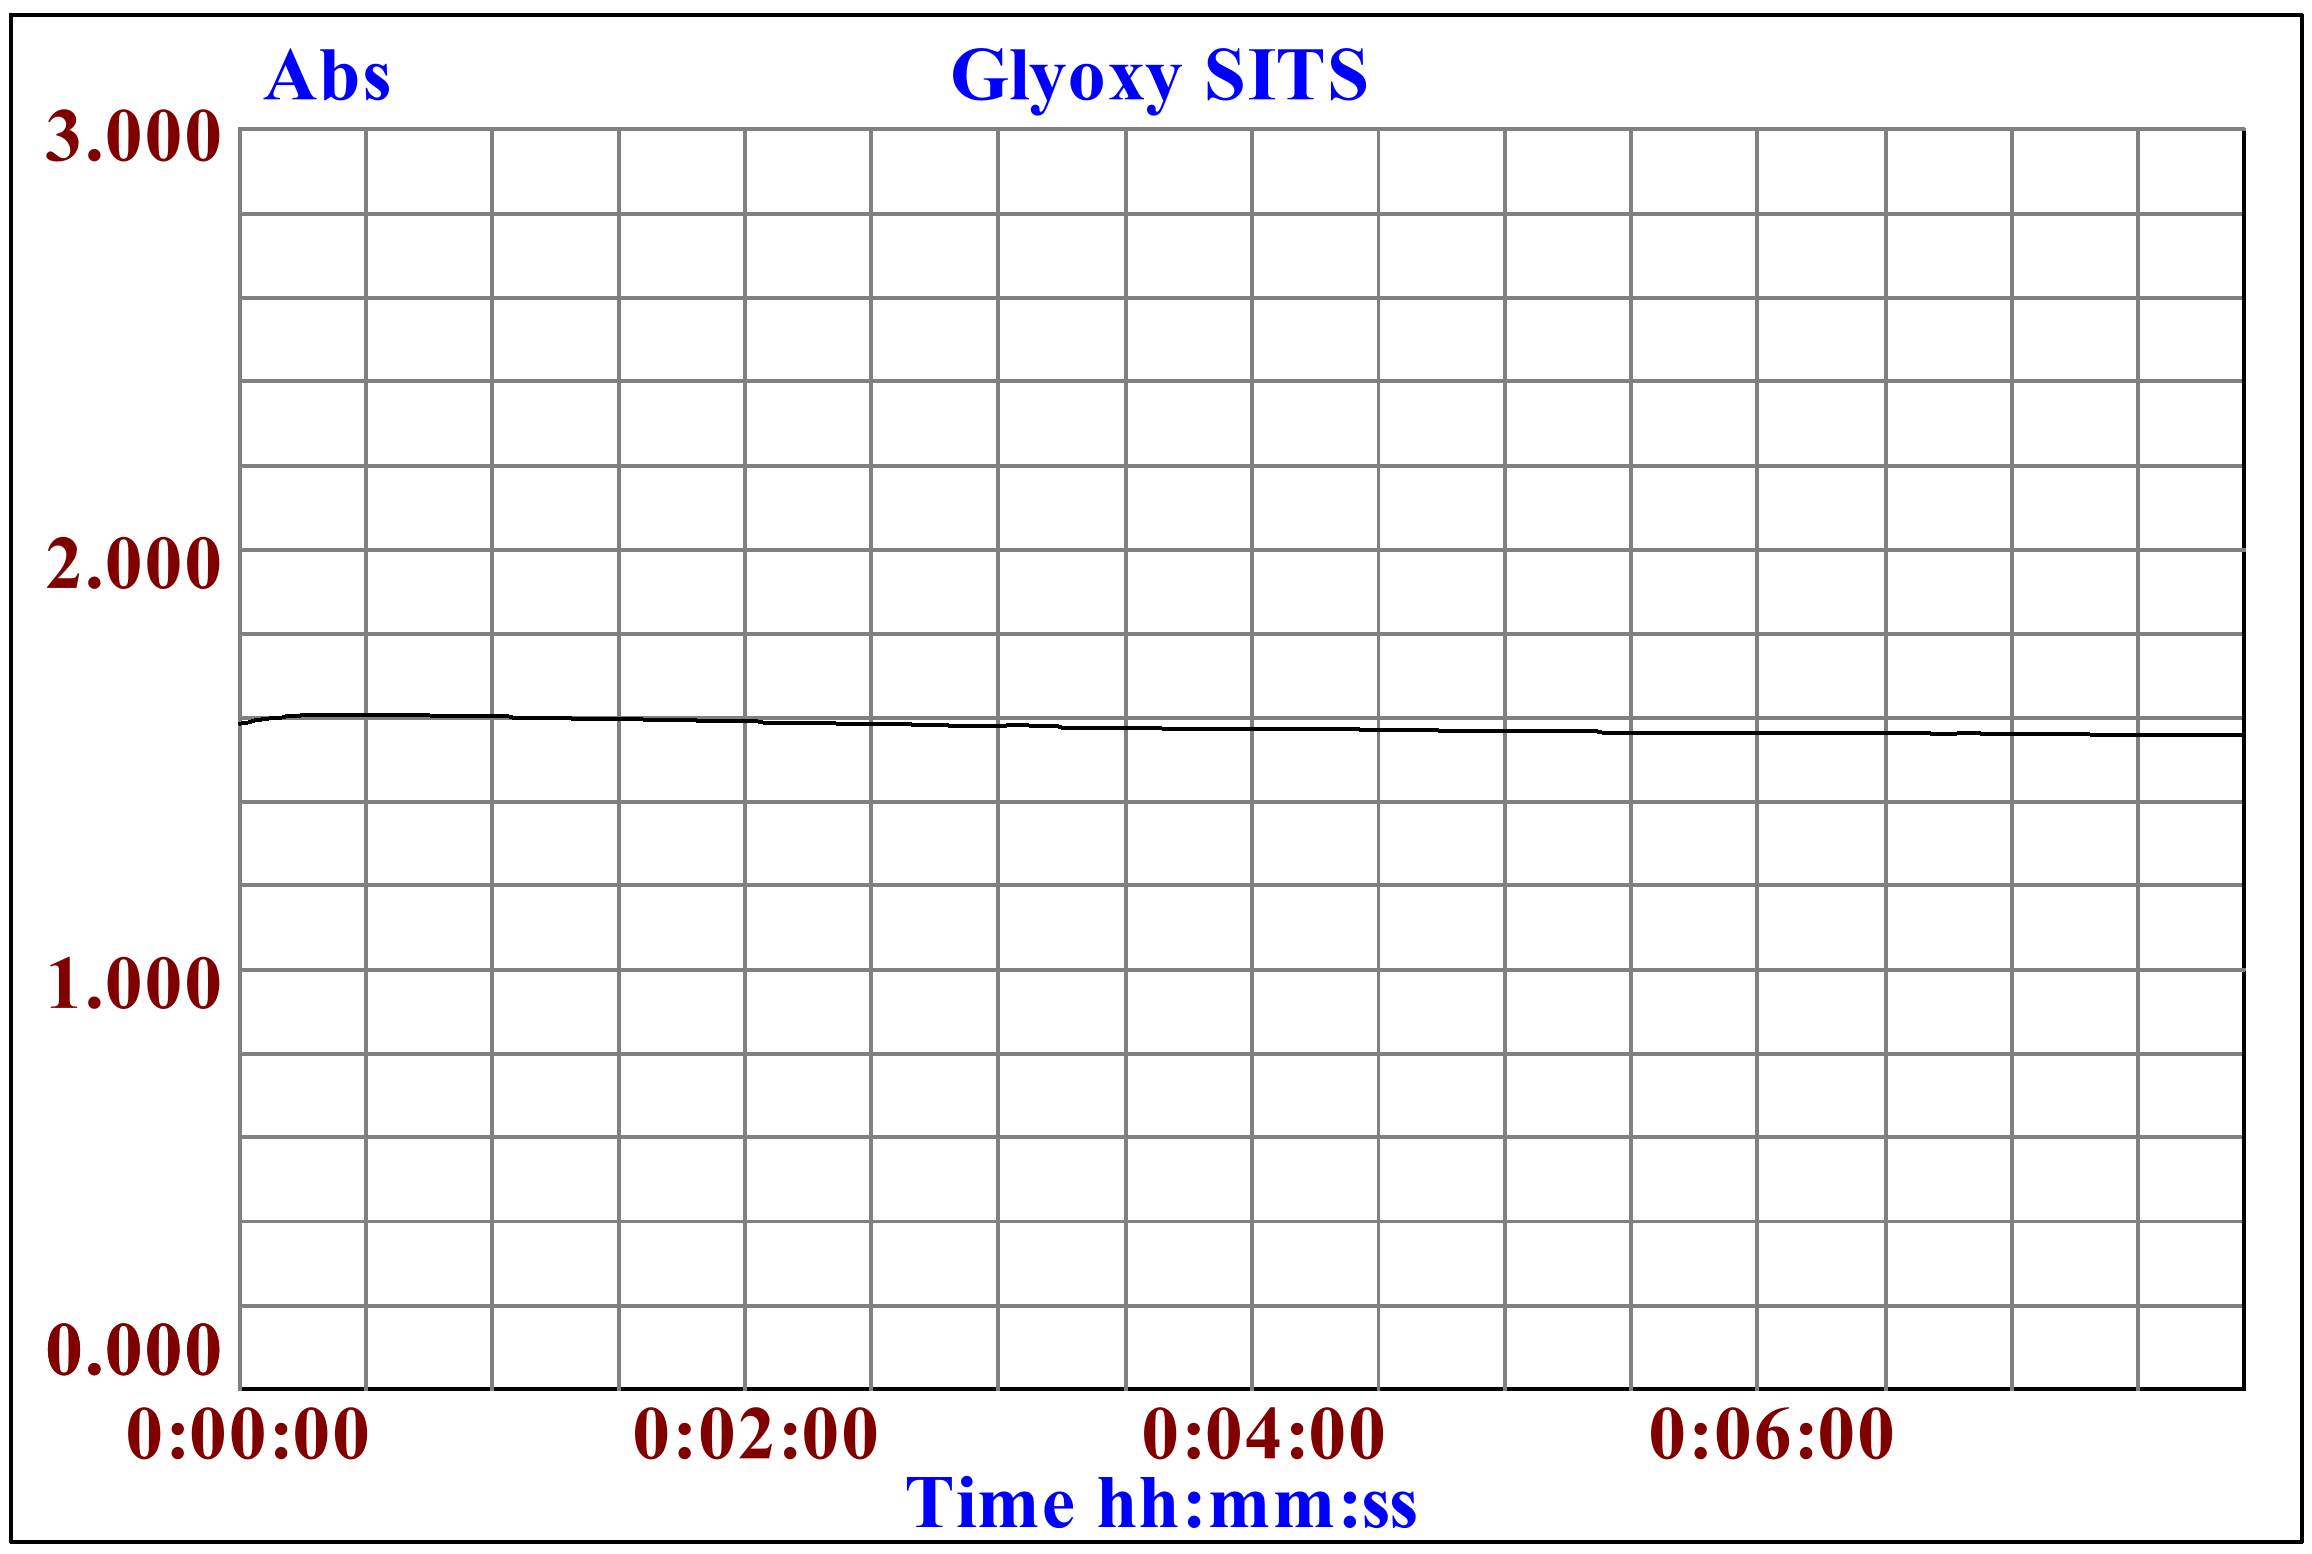
\includegraphics[width=\linewidth]{img/haem_glyoxy_sits.png}
		\caption{Glyoxylsäure \& SITS}
	\end{subfigure}
	\caption{Absorption von Glyoxylsäure bei \SI{610}{nm}}
	\label{fig:haem_glyoxy}
\end{figure}

\begin{figure}
	\centering
	\begin{subfigure}{.5\textwidth}
		\centering
		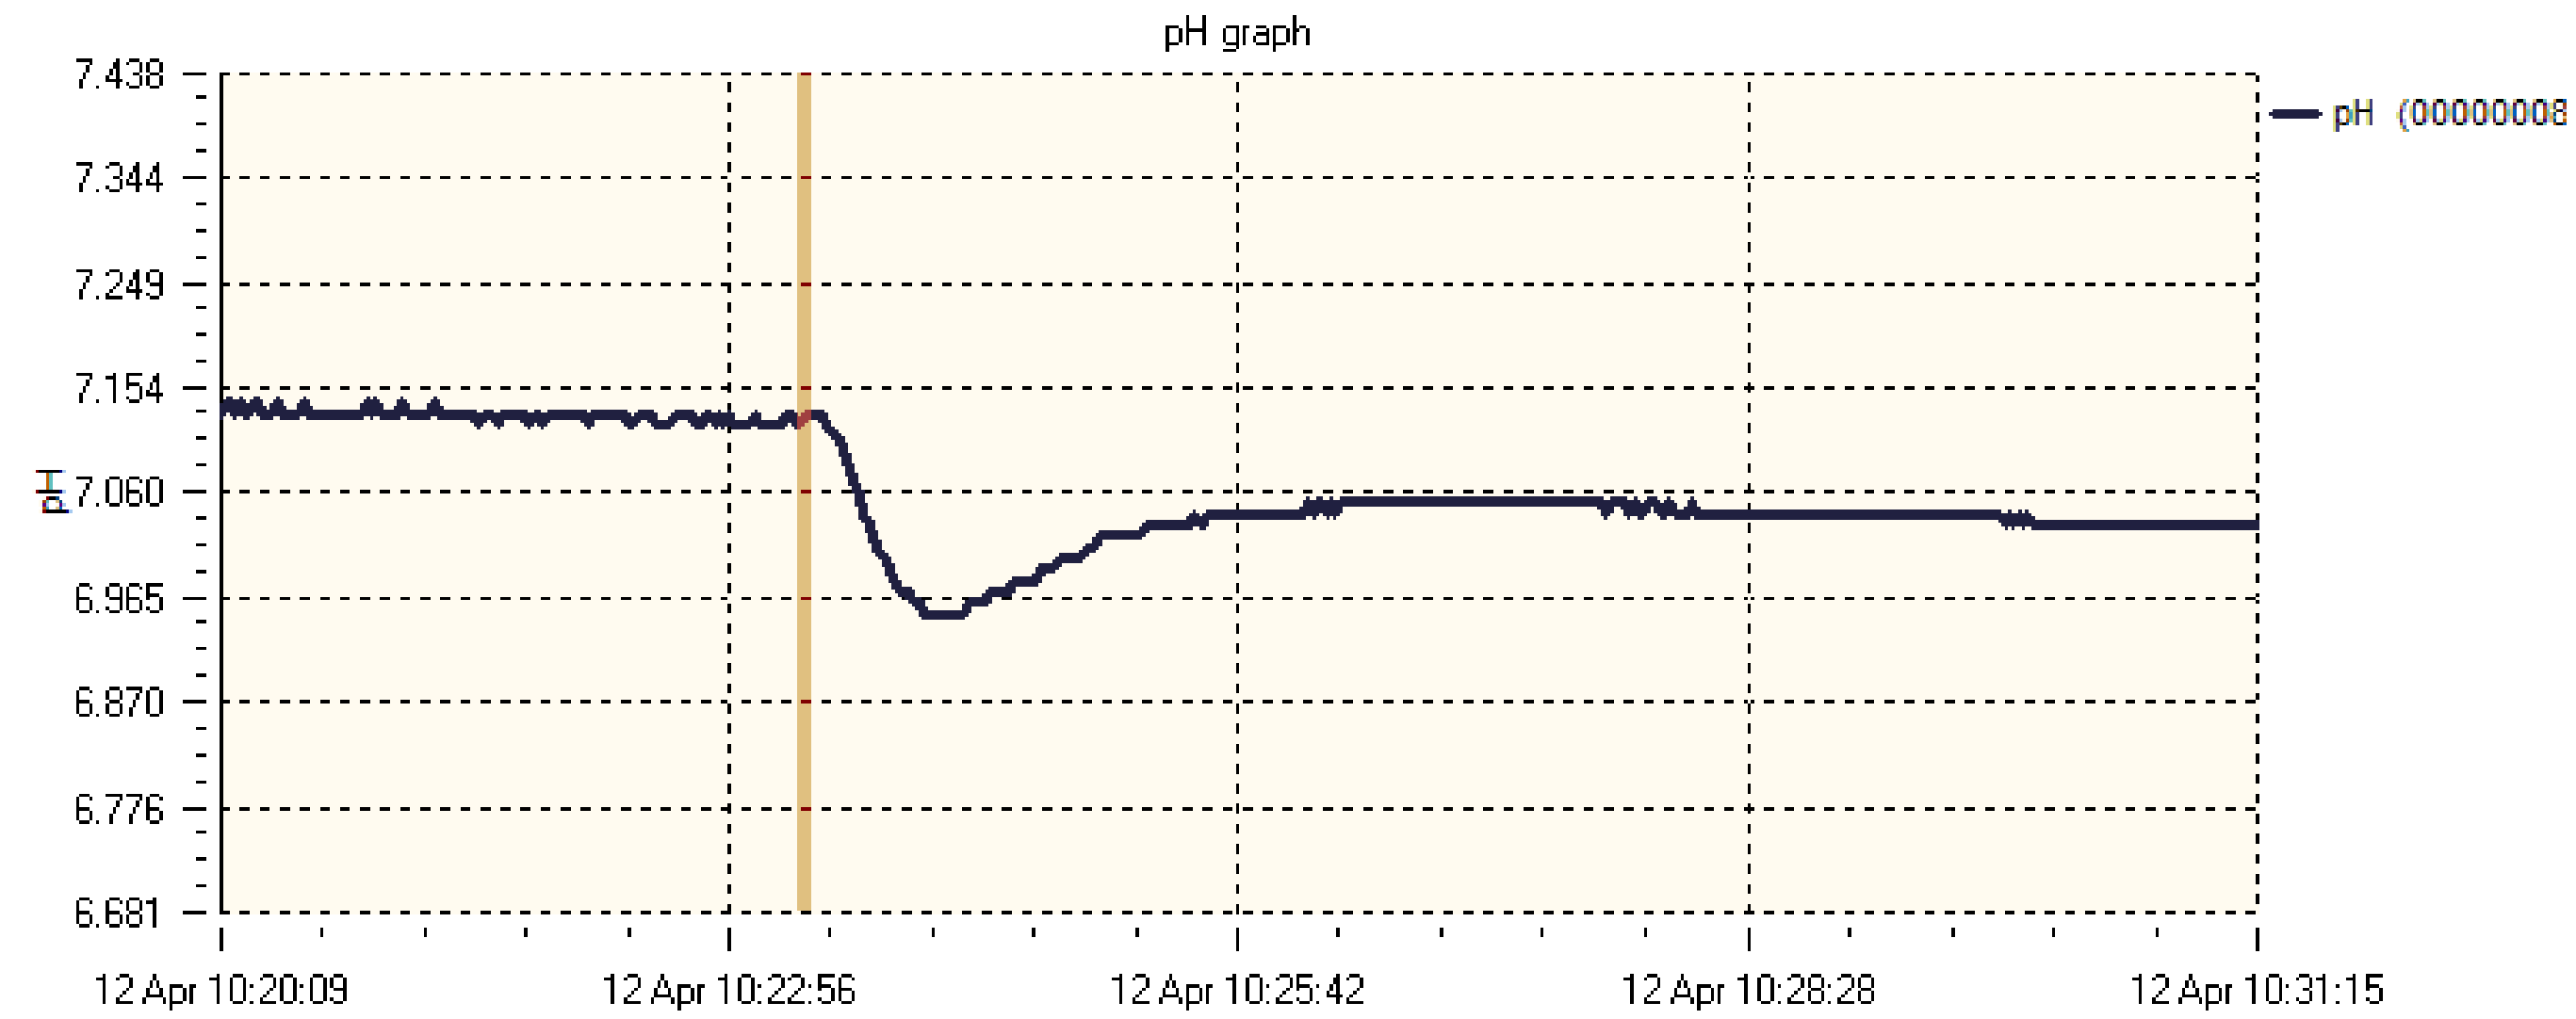
\includegraphics[width=\linewidth]{img/ph_glyoxy.png}
		\caption{Glyoxylsäure}
	\end{subfigure}%
	\begin{subfigure}{.5\textwidth}
		\centering
		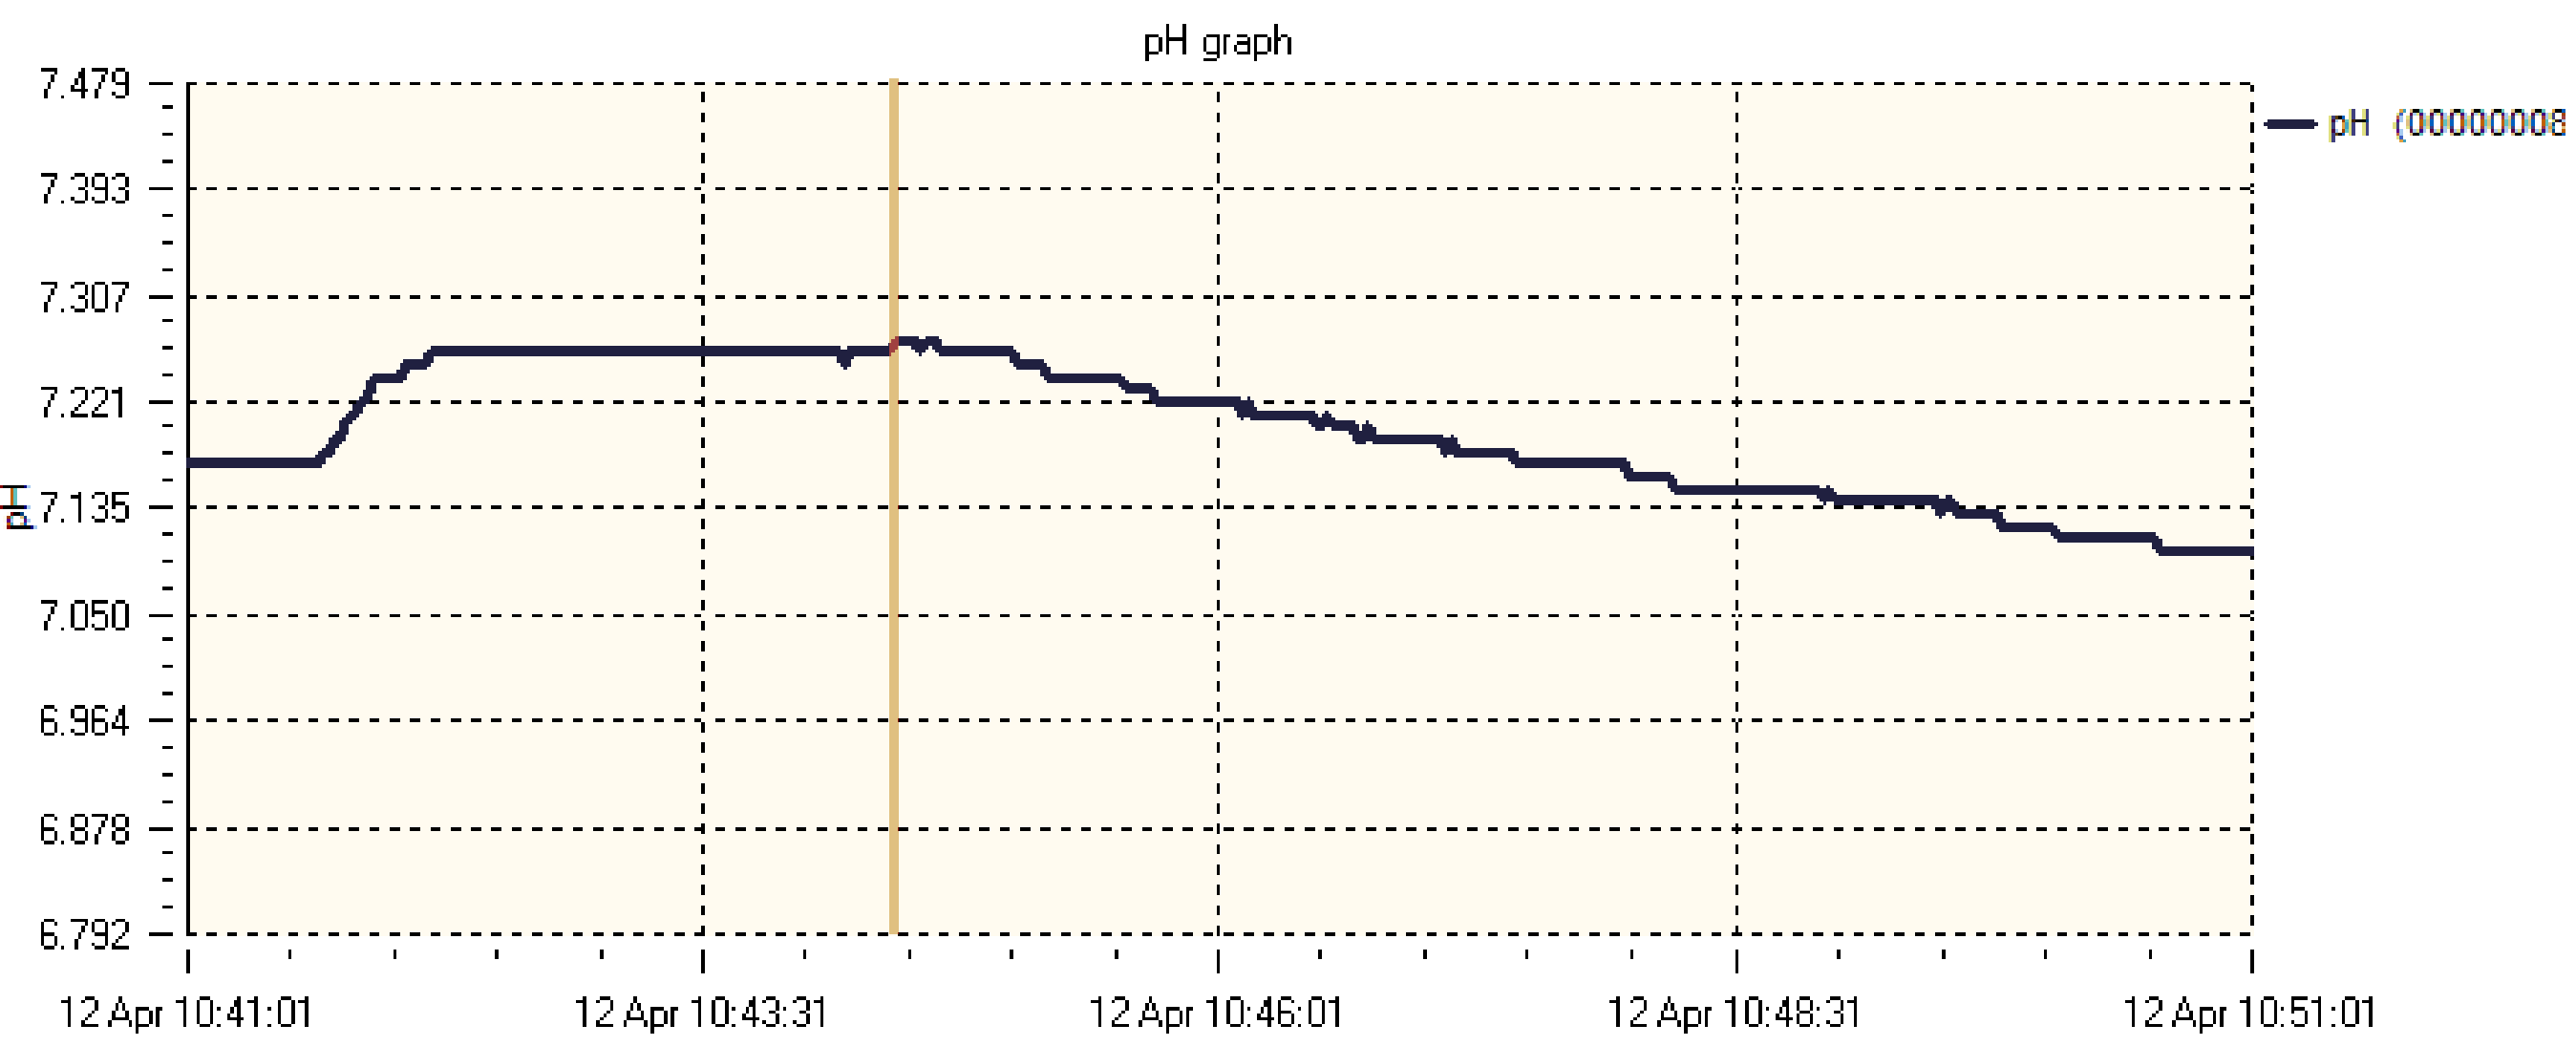
\includegraphics[width=\linewidth]{img/ph_glyoxy_sits.png}
		\caption{Glyoxylsäure \& SITS}
	\end{subfigure}
	\caption{Extrazellulärer pH von Glyoxylsäure}
	\label{fig:ph_glyoxy}
\end{figure}

Aus der Absorptionsmessung in Abbildung \ref{fig:haem_glyoxy} ist ersichtlich,
dass es nur zur Hämolyse kam wenn kein SITS im System war. Dies impliziert,
dass Glyoxylsäure via Bande-3 Protein die Zelle betritt.

Dies lässt sich auch mit der pH Messung des Assays ohne SITS in Abbildung
\ref{fig:ph_glyoxy} bestätigen, in welcher der pH zuerst absinkt, sich dann
aber wieder in einem neuen Gleichgewicht einfindet.

Die pH Messung des Assays mit SITS sinkt - anders als erwartet - mit der Zeit
leicht ab, was darauf hindeuten könnte, dass zu wenig SITS im Assay vorhanden
war, oder zu wenig gemischt wurde.

\subsection{Weinsäure}

\begin{figure}
	\centering
	\begin{subfigure}{.5\textwidth}
		\centering
		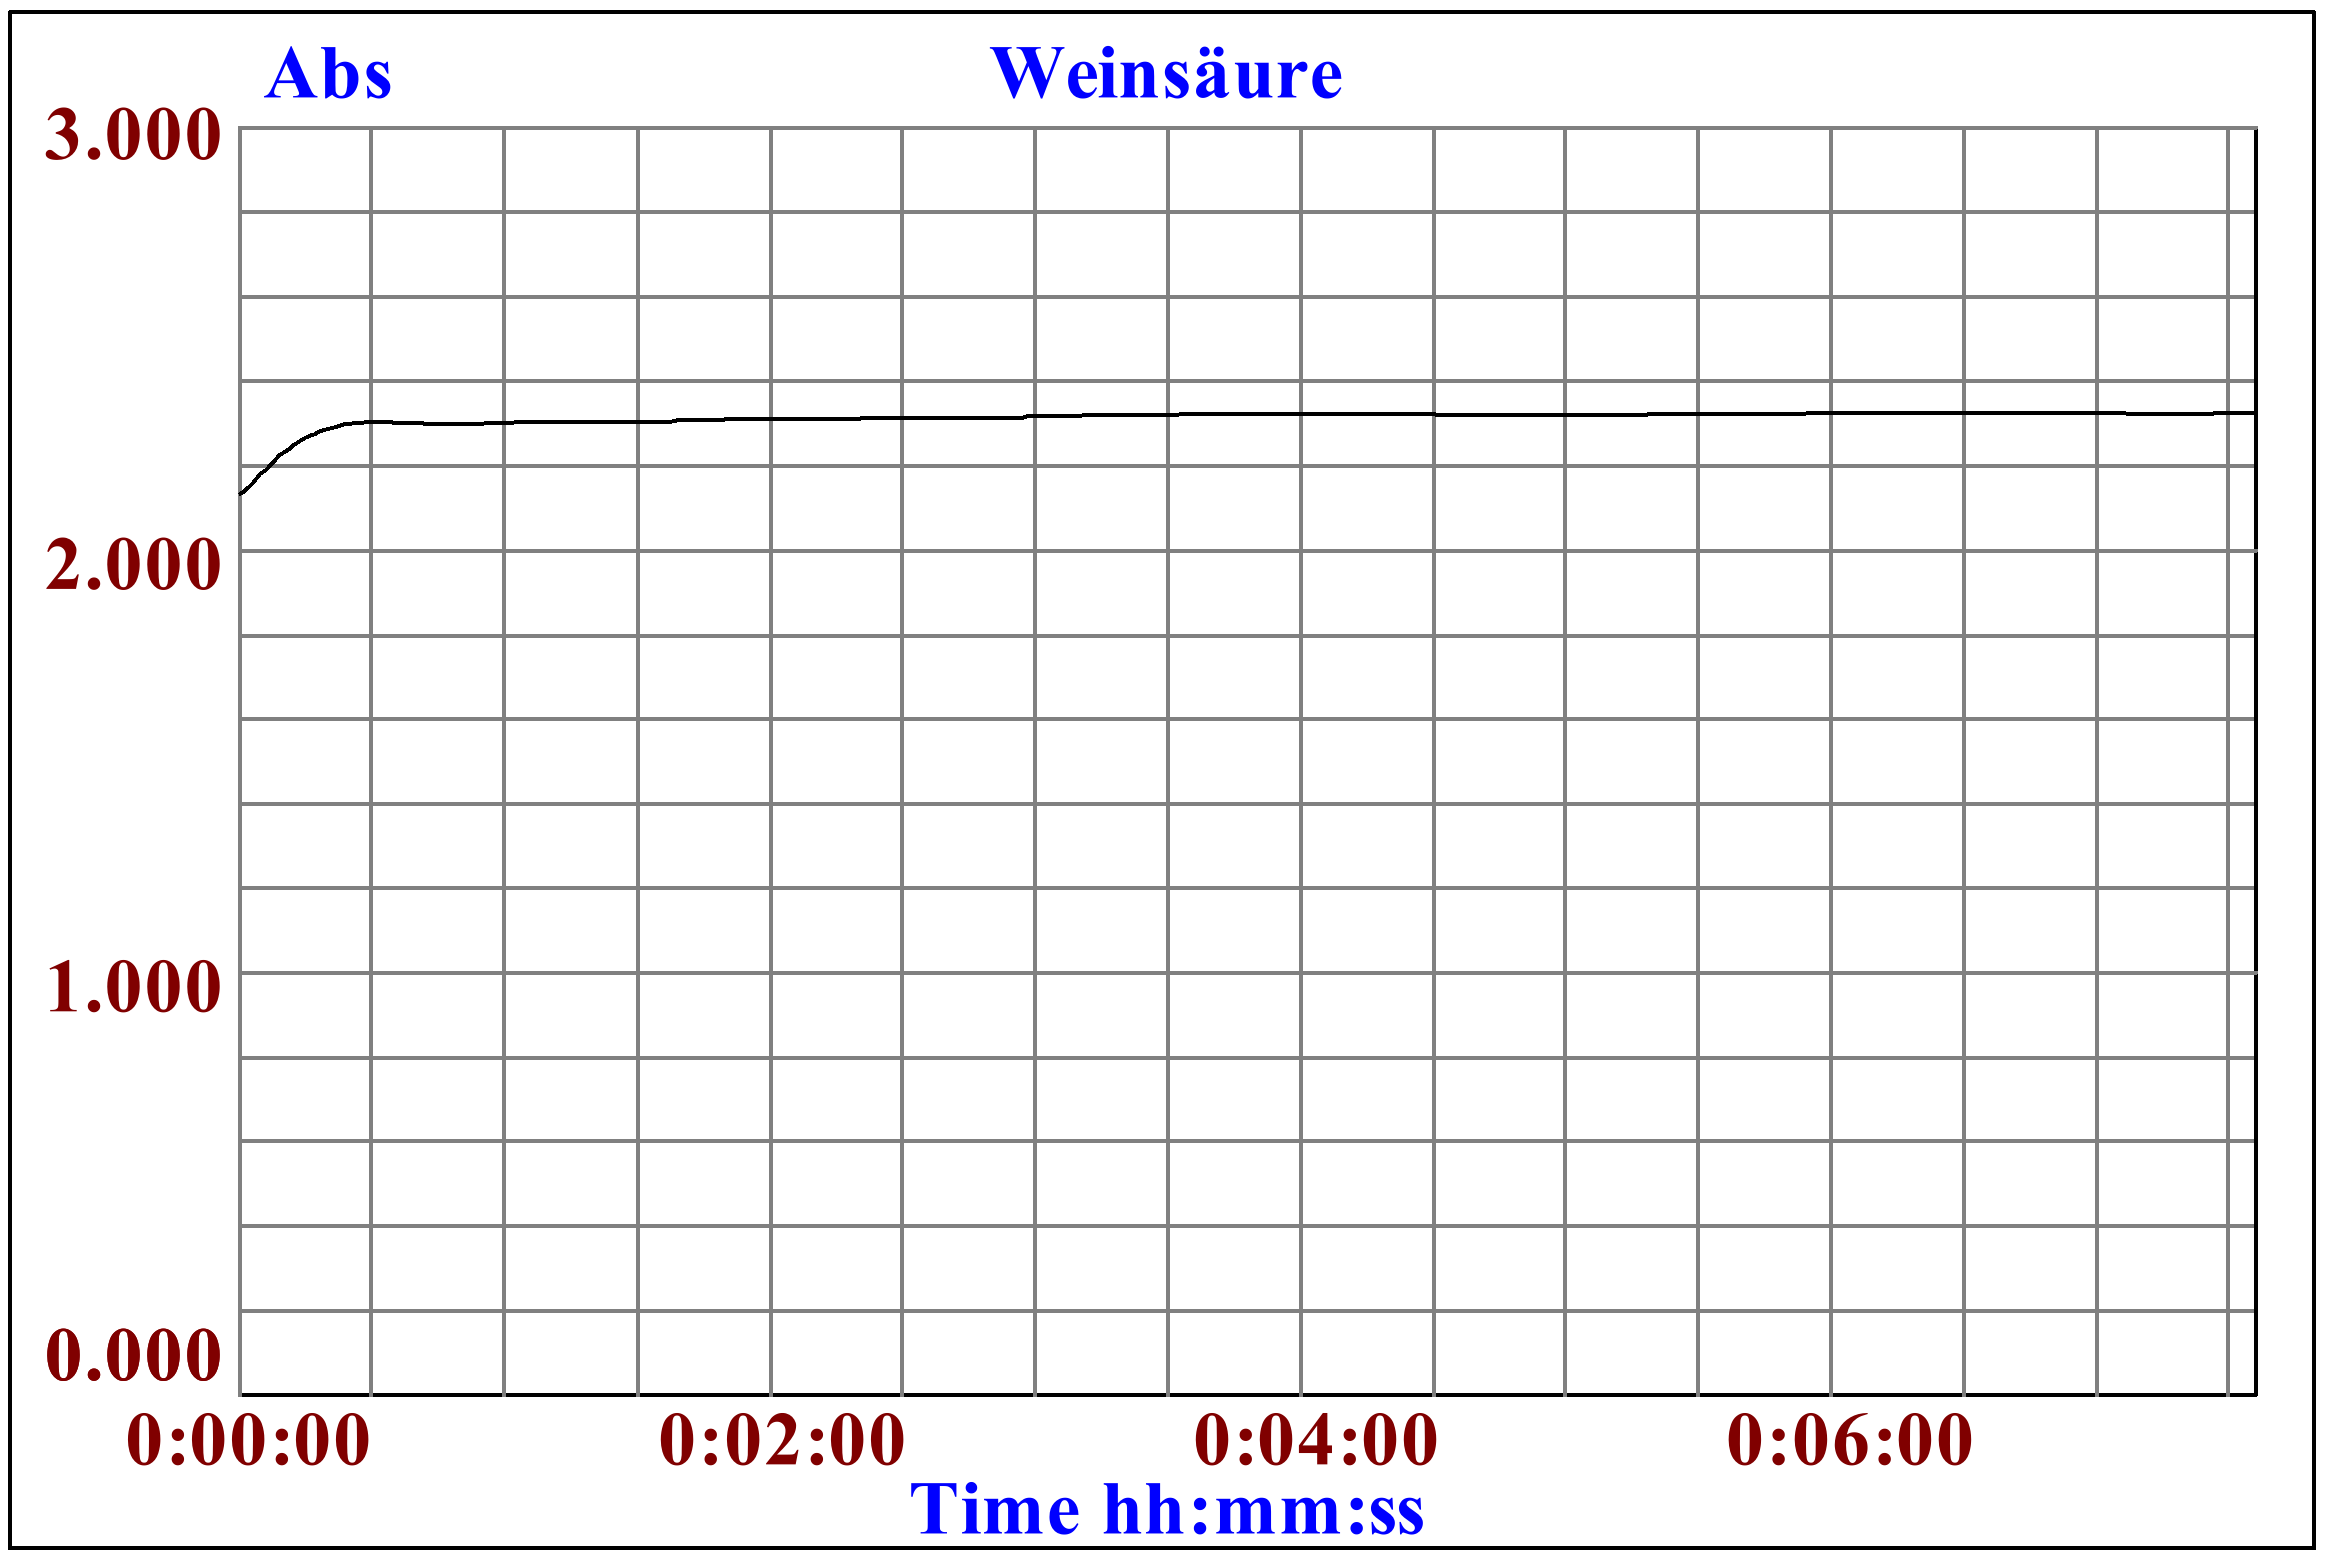
\includegraphics[width=\linewidth]{img/haem_wein.png}
		\caption{Weinsäure}
	\end{subfigure}%
	\begin{subfigure}{.5\textwidth}
		\centering
		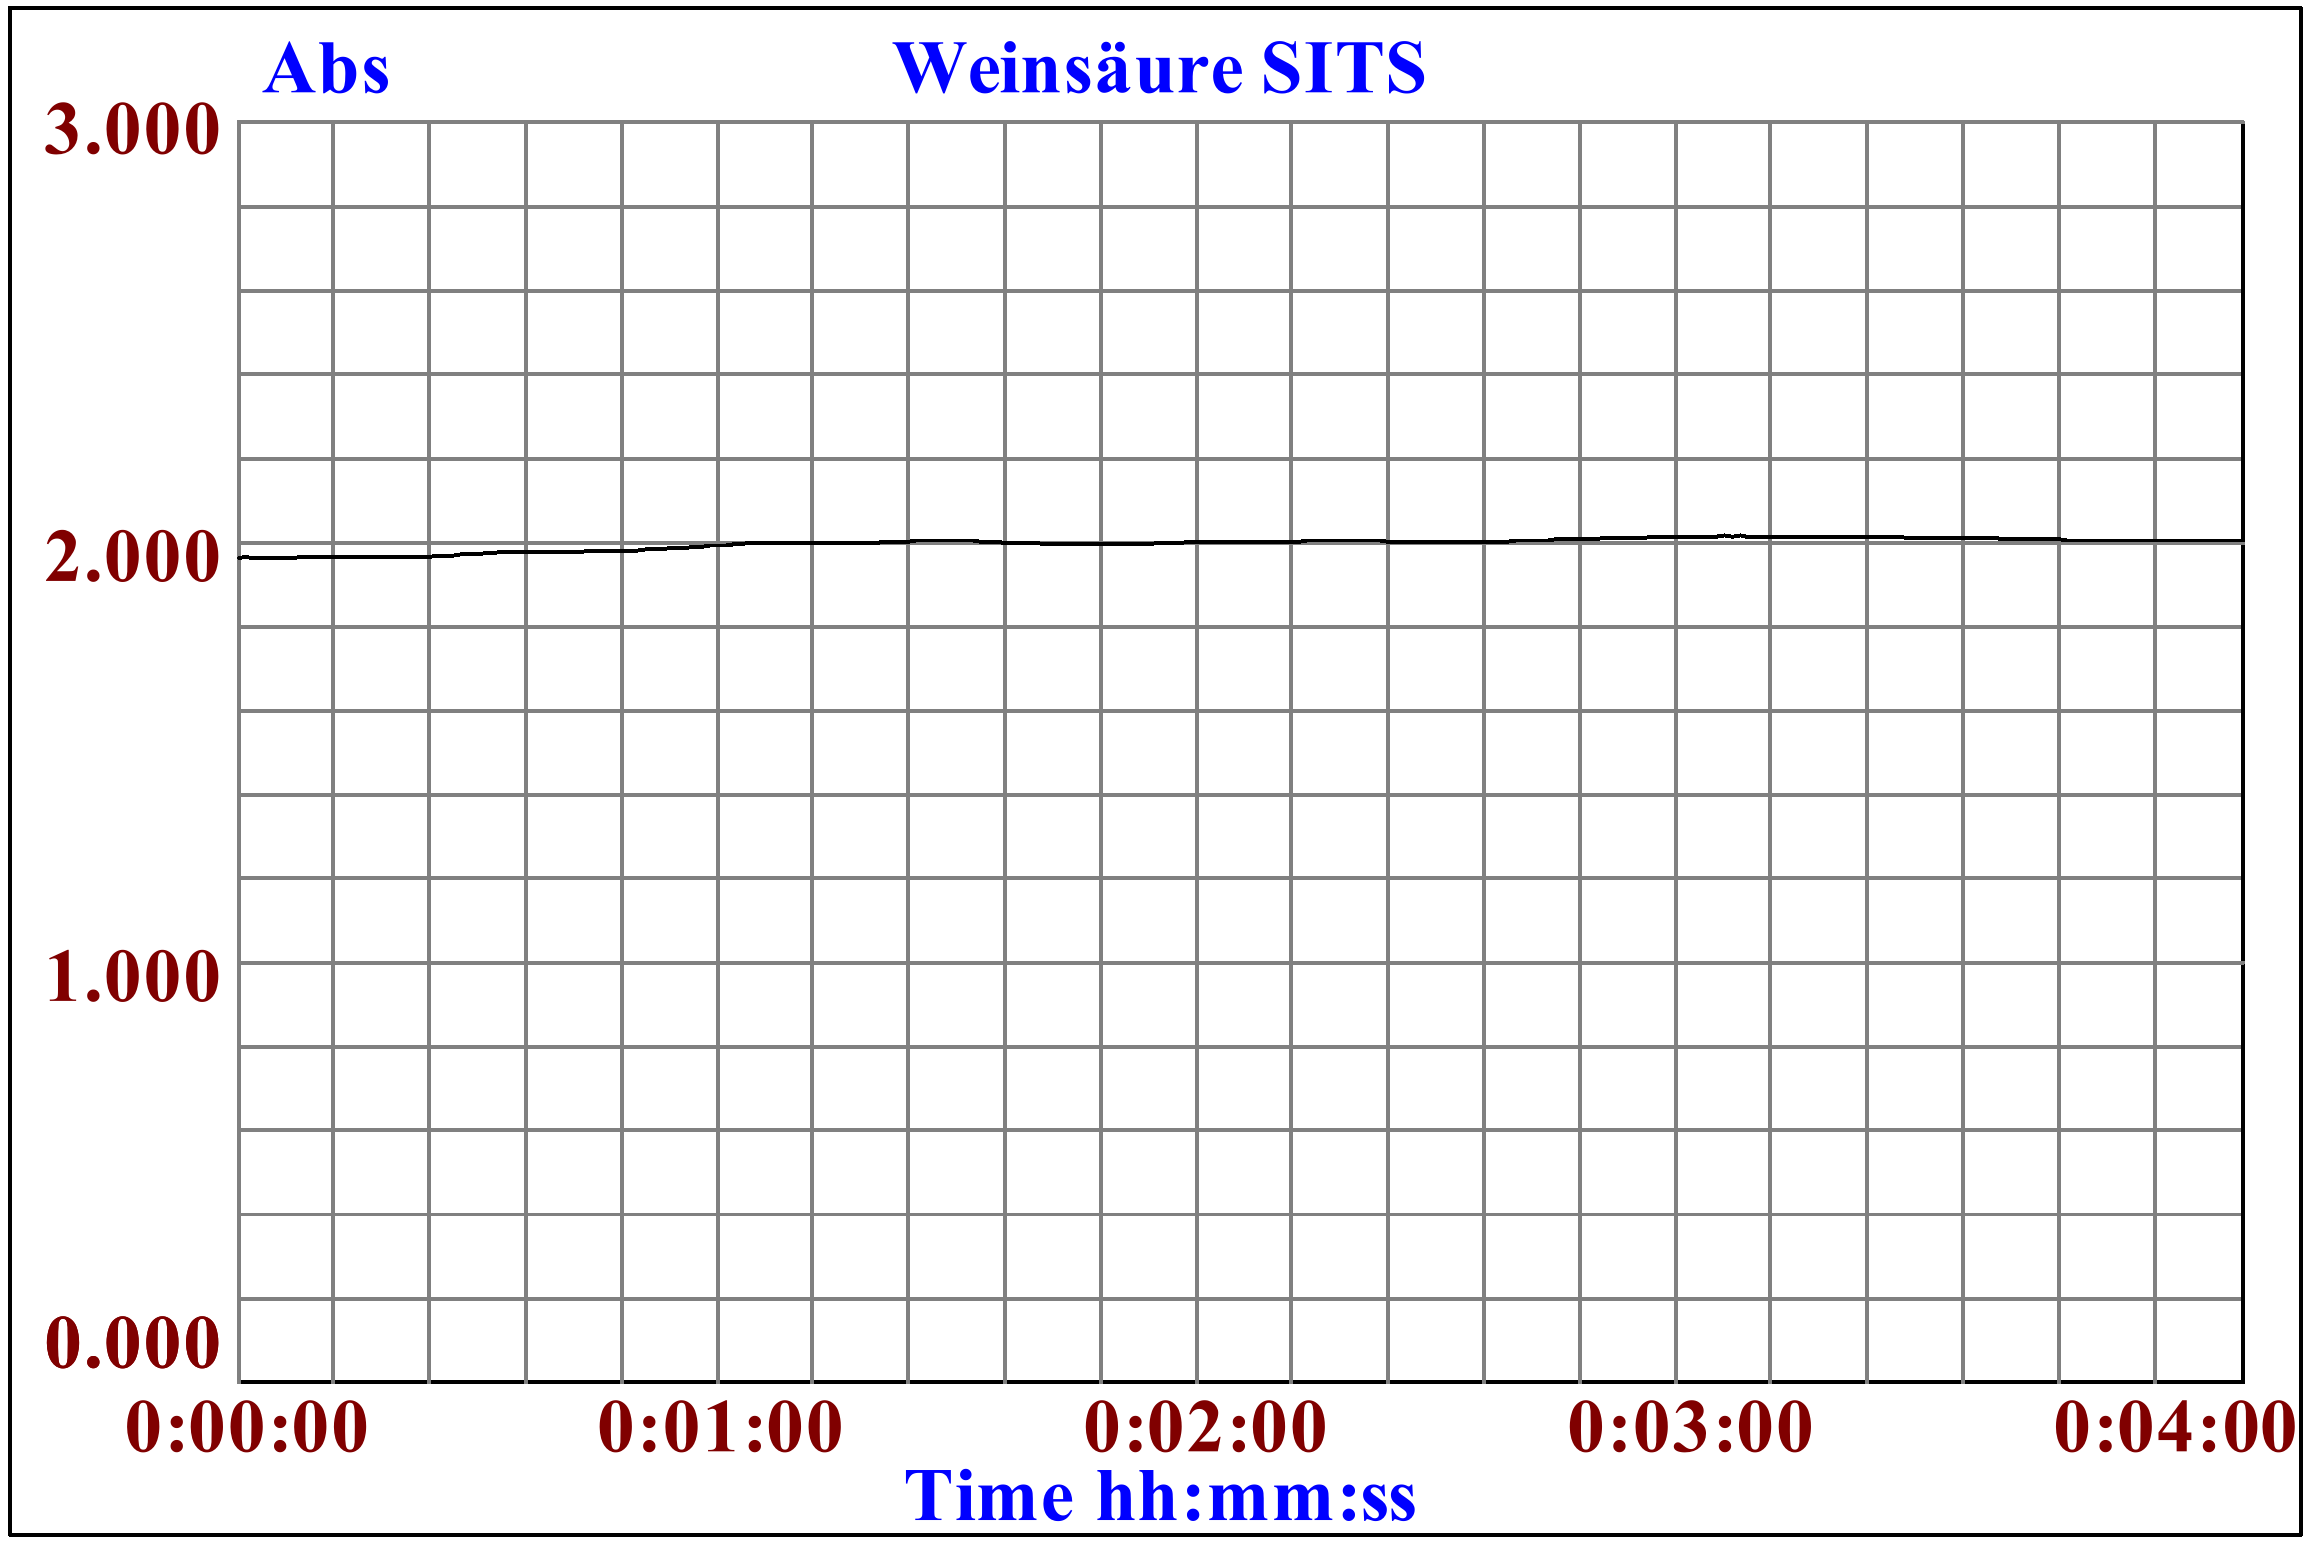
\includegraphics[width=\linewidth]{img/haem_wein_sits.png}
		\caption{Weinsäure \& SITS}
	\end{subfigure}
	\caption{Absorption von Weinsäure bei \SI{610}{nm}}
	\label{fig:haem_wein}
\end{figure}

\begin{figure}
	\centering
	\begin{subfigure}{.5\textwidth}
		\centering
		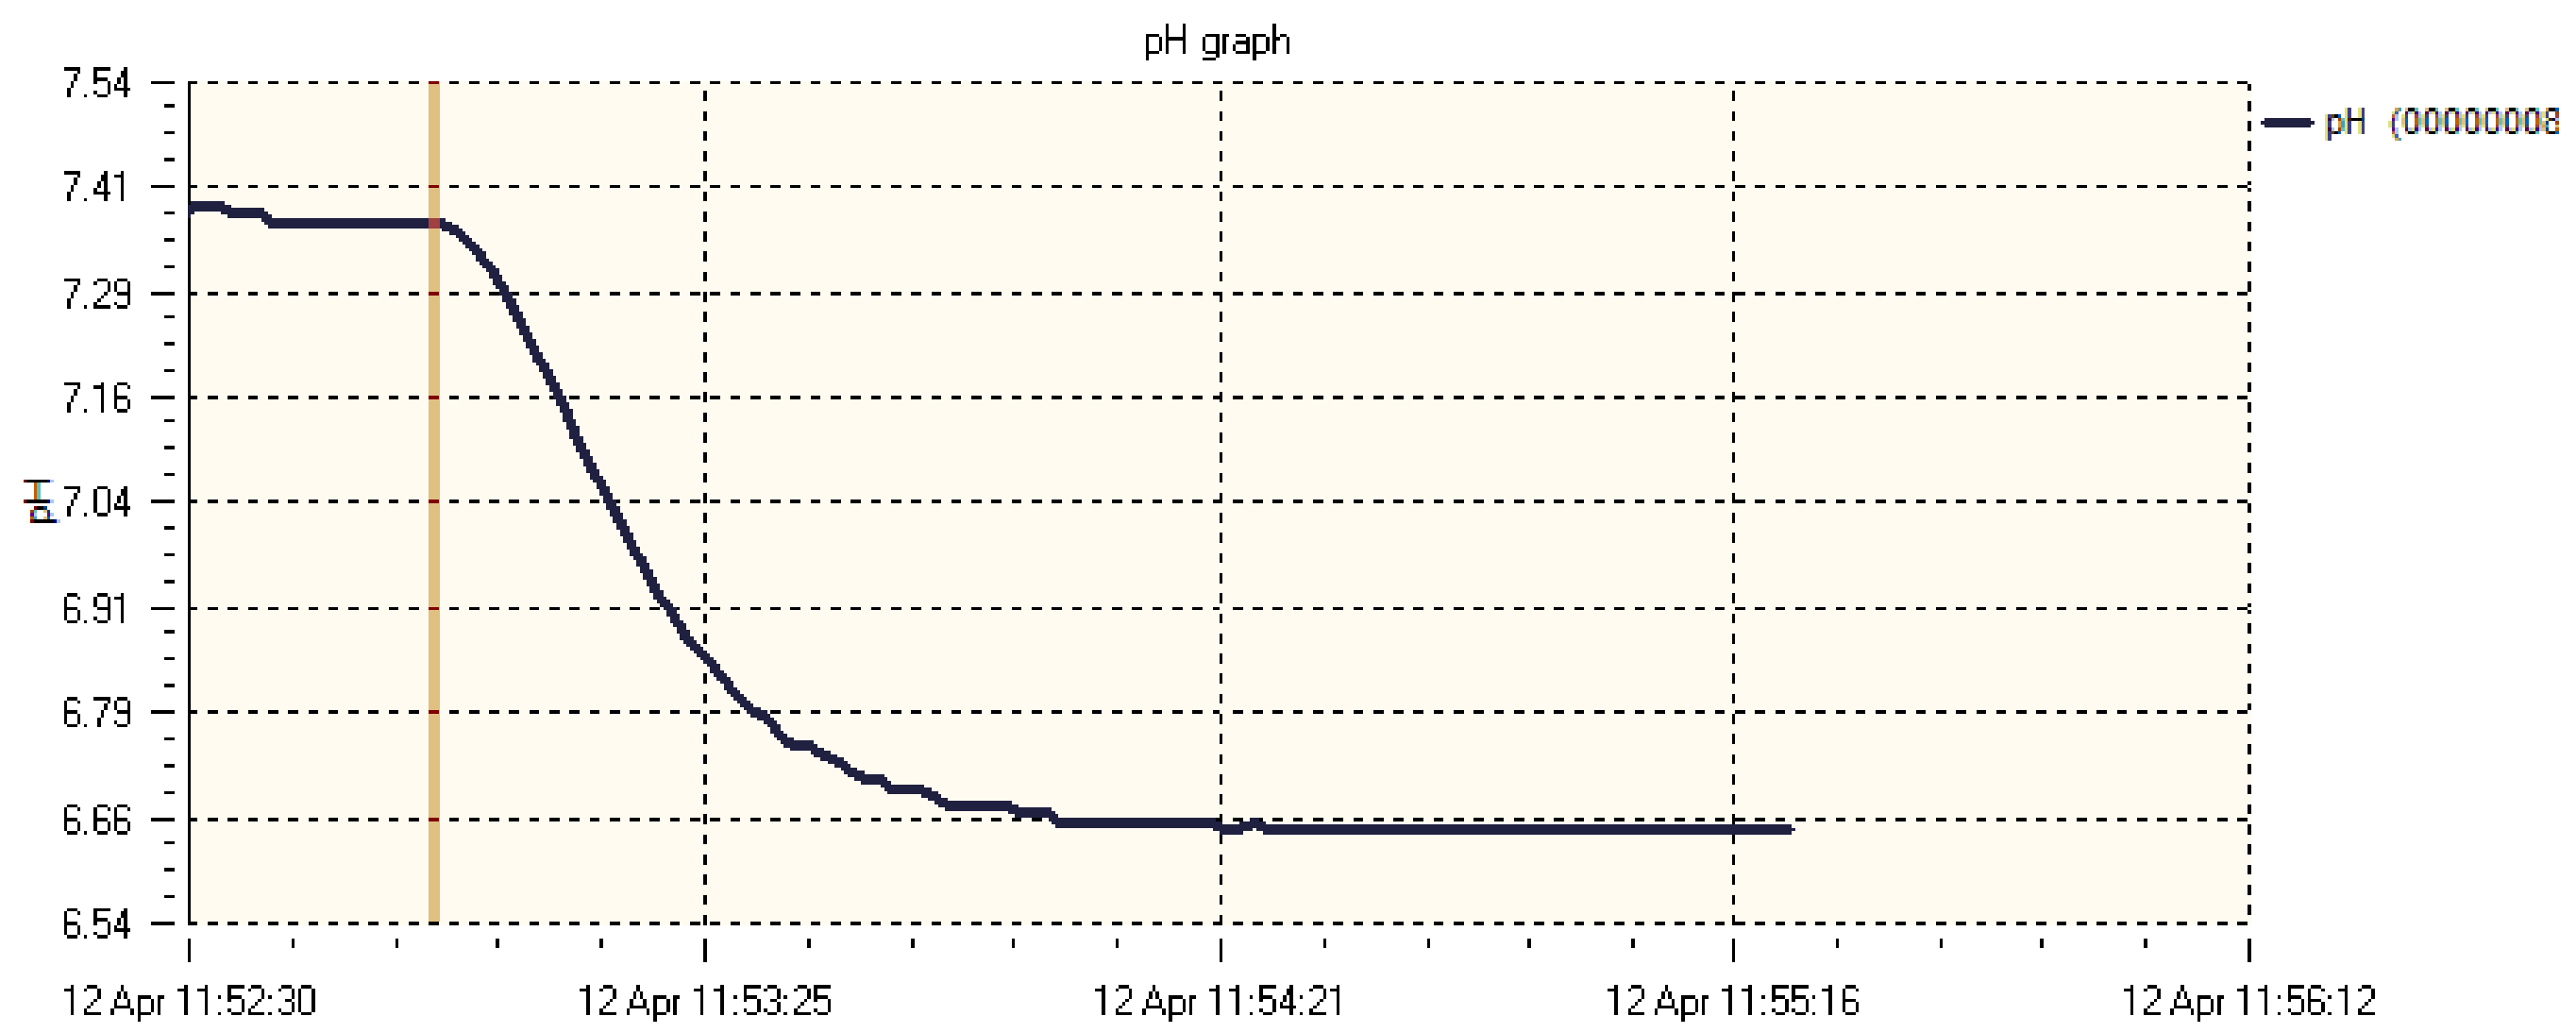
\includegraphics[width=\linewidth]{img/ph_wein.png}
		\caption{Weinsäure}
	\end{subfigure}%
	\begin{subfigure}{.5\textwidth}
		\centering
		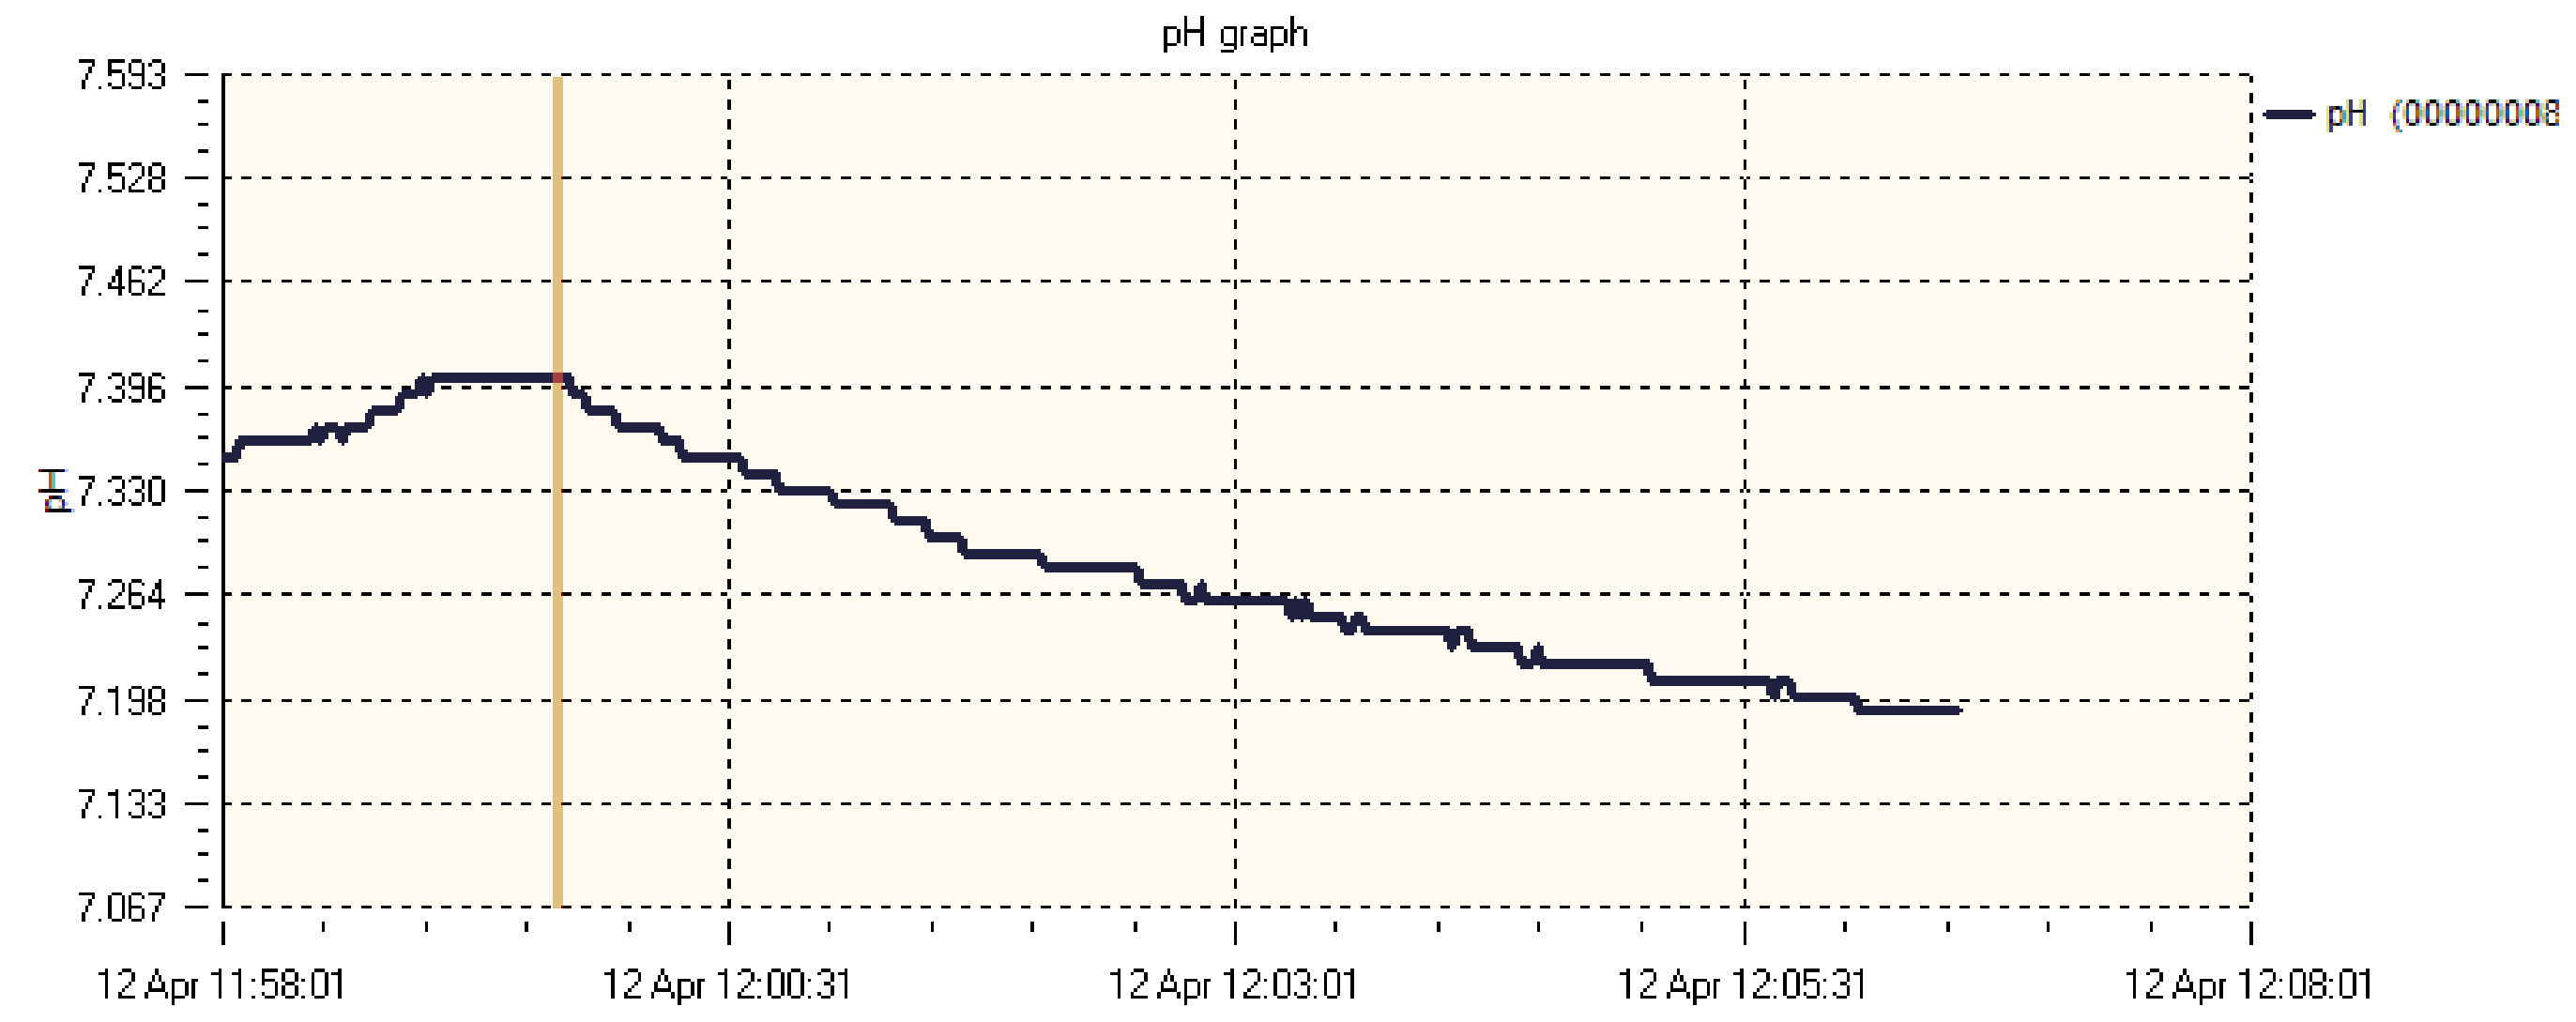
\includegraphics[width=\linewidth]{img/ph_wein_sits.png}
		\caption{Weinsäure \& SITS}
	\end{subfigure}
	\caption{Extrazellulärer pH von Weinsäure}
	\label{fig:ph_wein}
\end{figure}

Aus der Absorptionsmessung in Abbildung \ref{fig:haem_wein} ist ersichtlich,
dass es nicht zur Hämolyse kam. Dies impliziert, dass Weinsäure weder via
Bande-3 noch via Diffusion in die Zelle transportiert wird.

Dies lässt sich auch mit der pH Messung in Abbildung \ref{fig:ph_wein}
bestätigen, in welcher im Falle des Assays ohne SITS der pH aufgrund des
Austausches von \ce{Cl-} und \ce{OH-} sinkt, aber - da keine Säure die Zelle
betreten kann - nicht wieder ansteigt.

\subsection{Zitronensäure}

\begin{figure}
	\centering
	\begin{subfigure}{.5\textwidth}
		\centering
		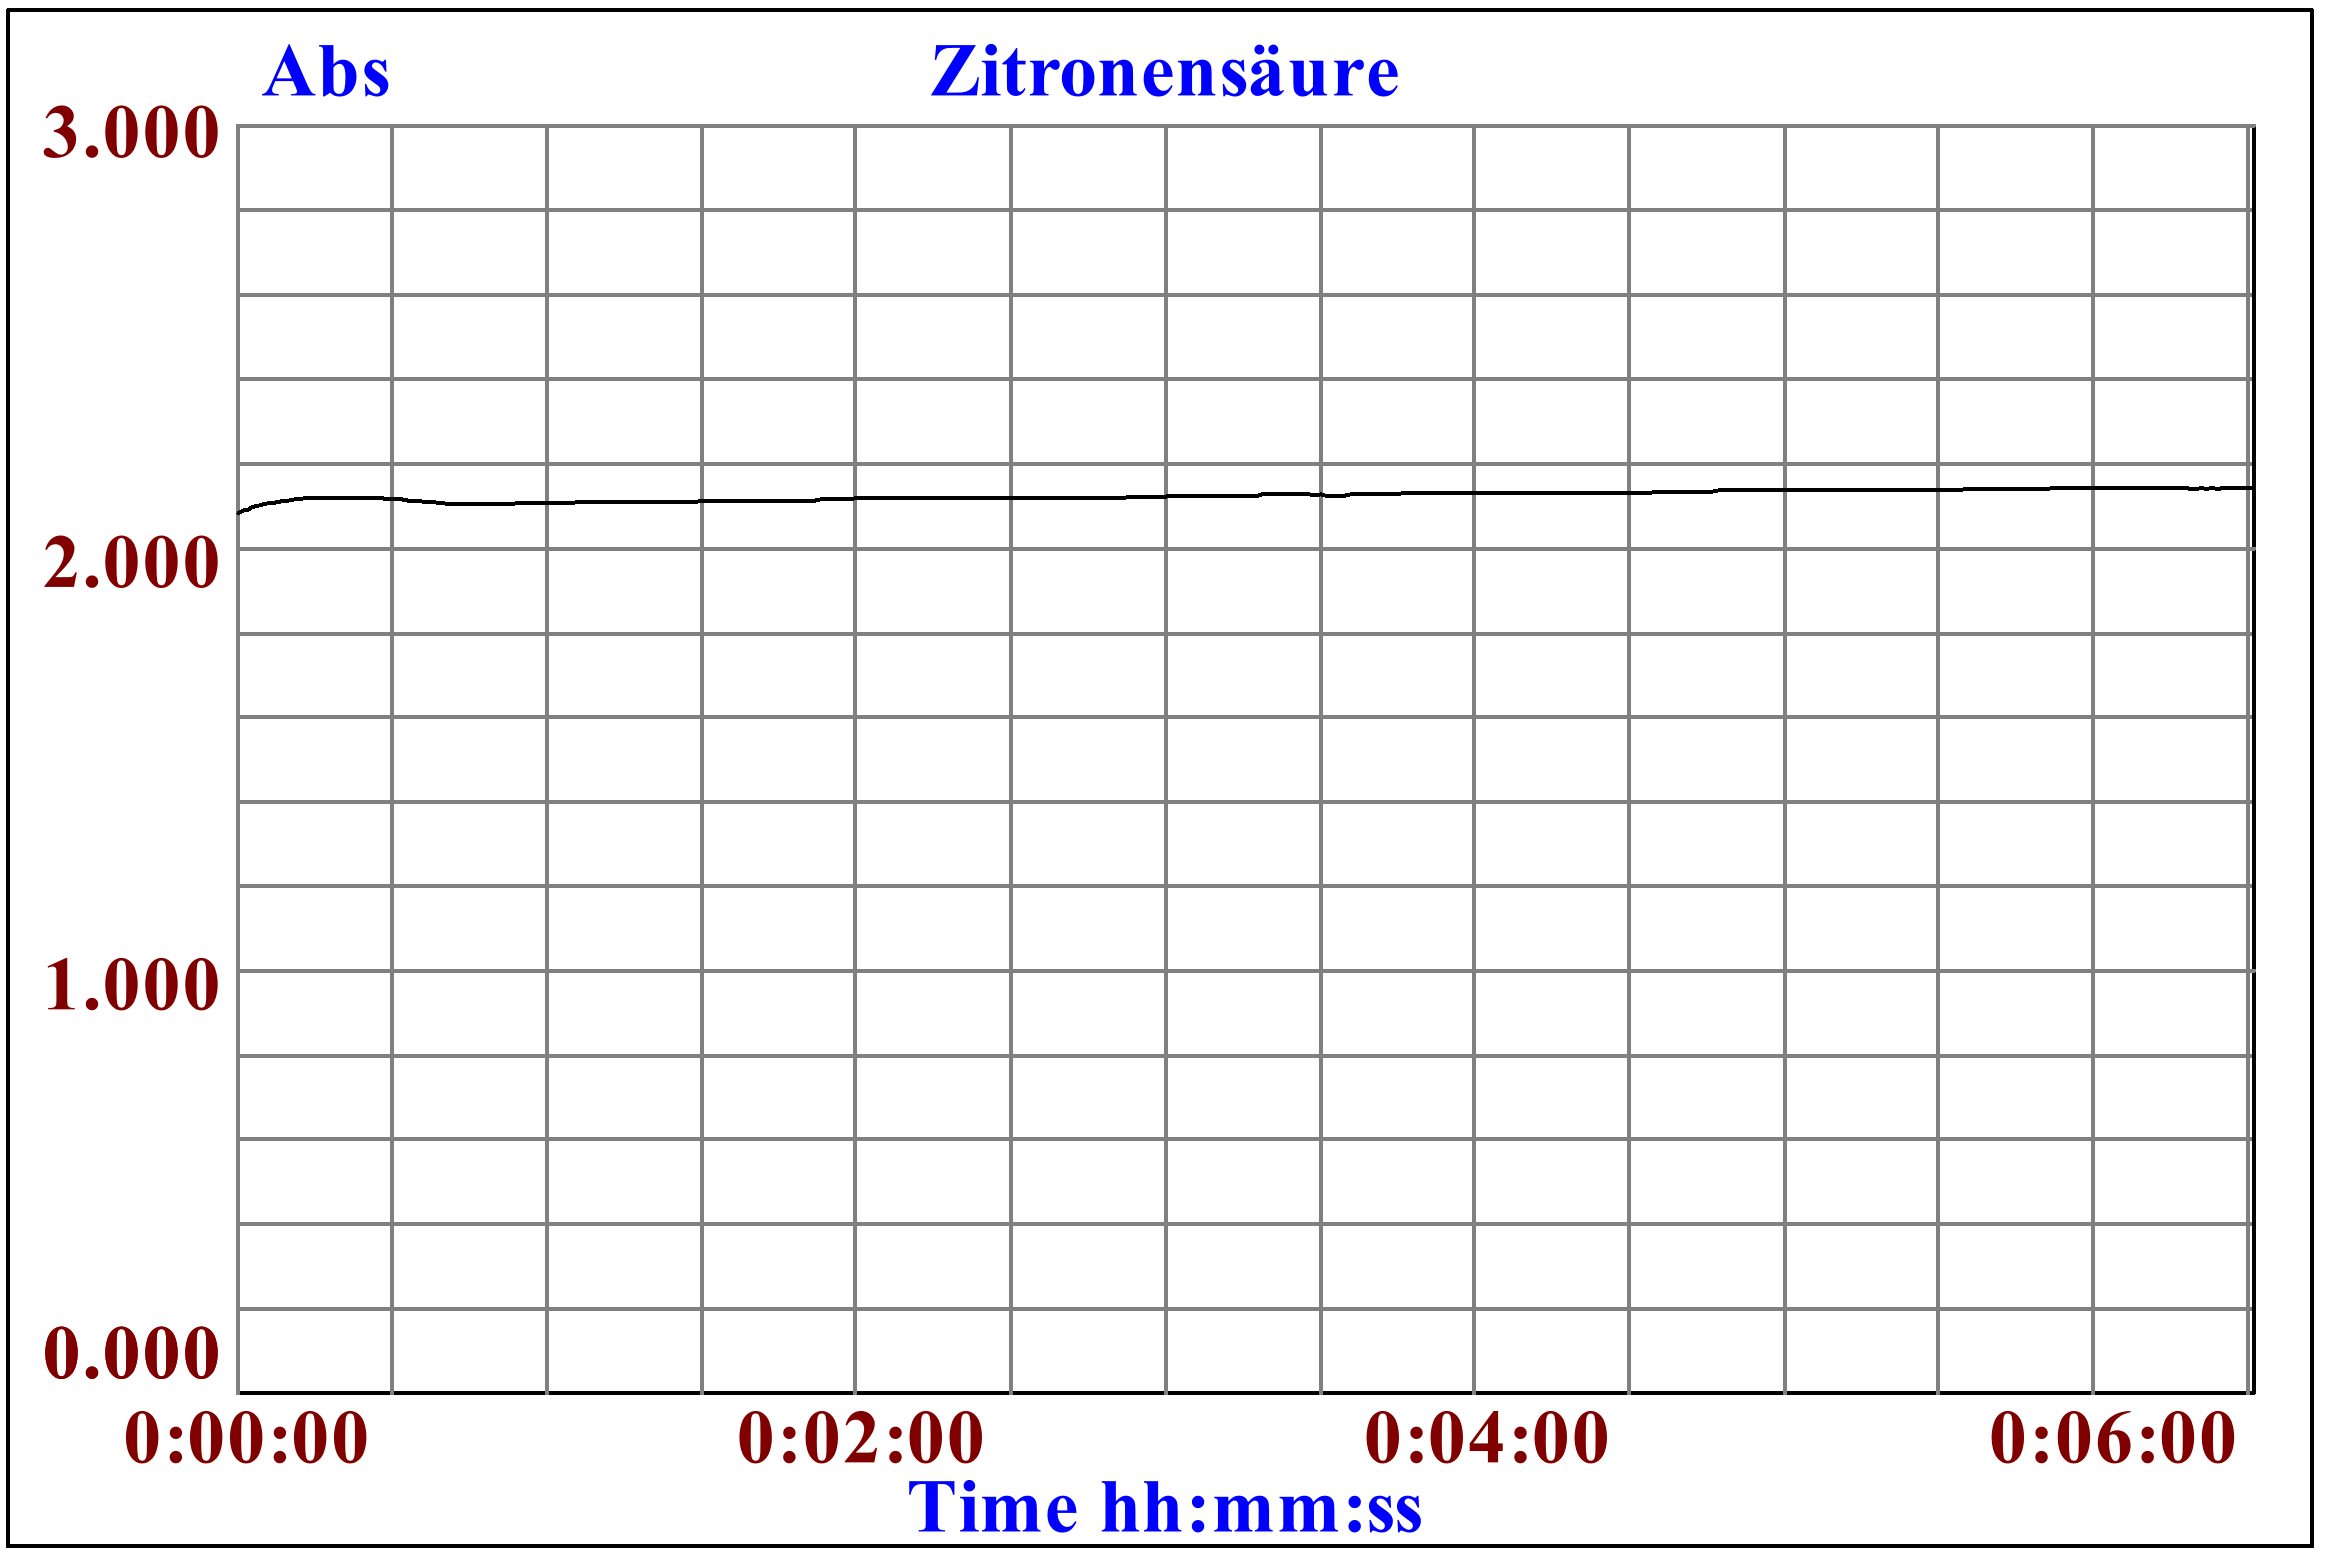
\includegraphics[width=\linewidth]{img/haem_citric.png}
		\caption{Zitronensäure}
	\end{subfigure}%
	\begin{subfigure}{.5\textwidth}
		\centering
		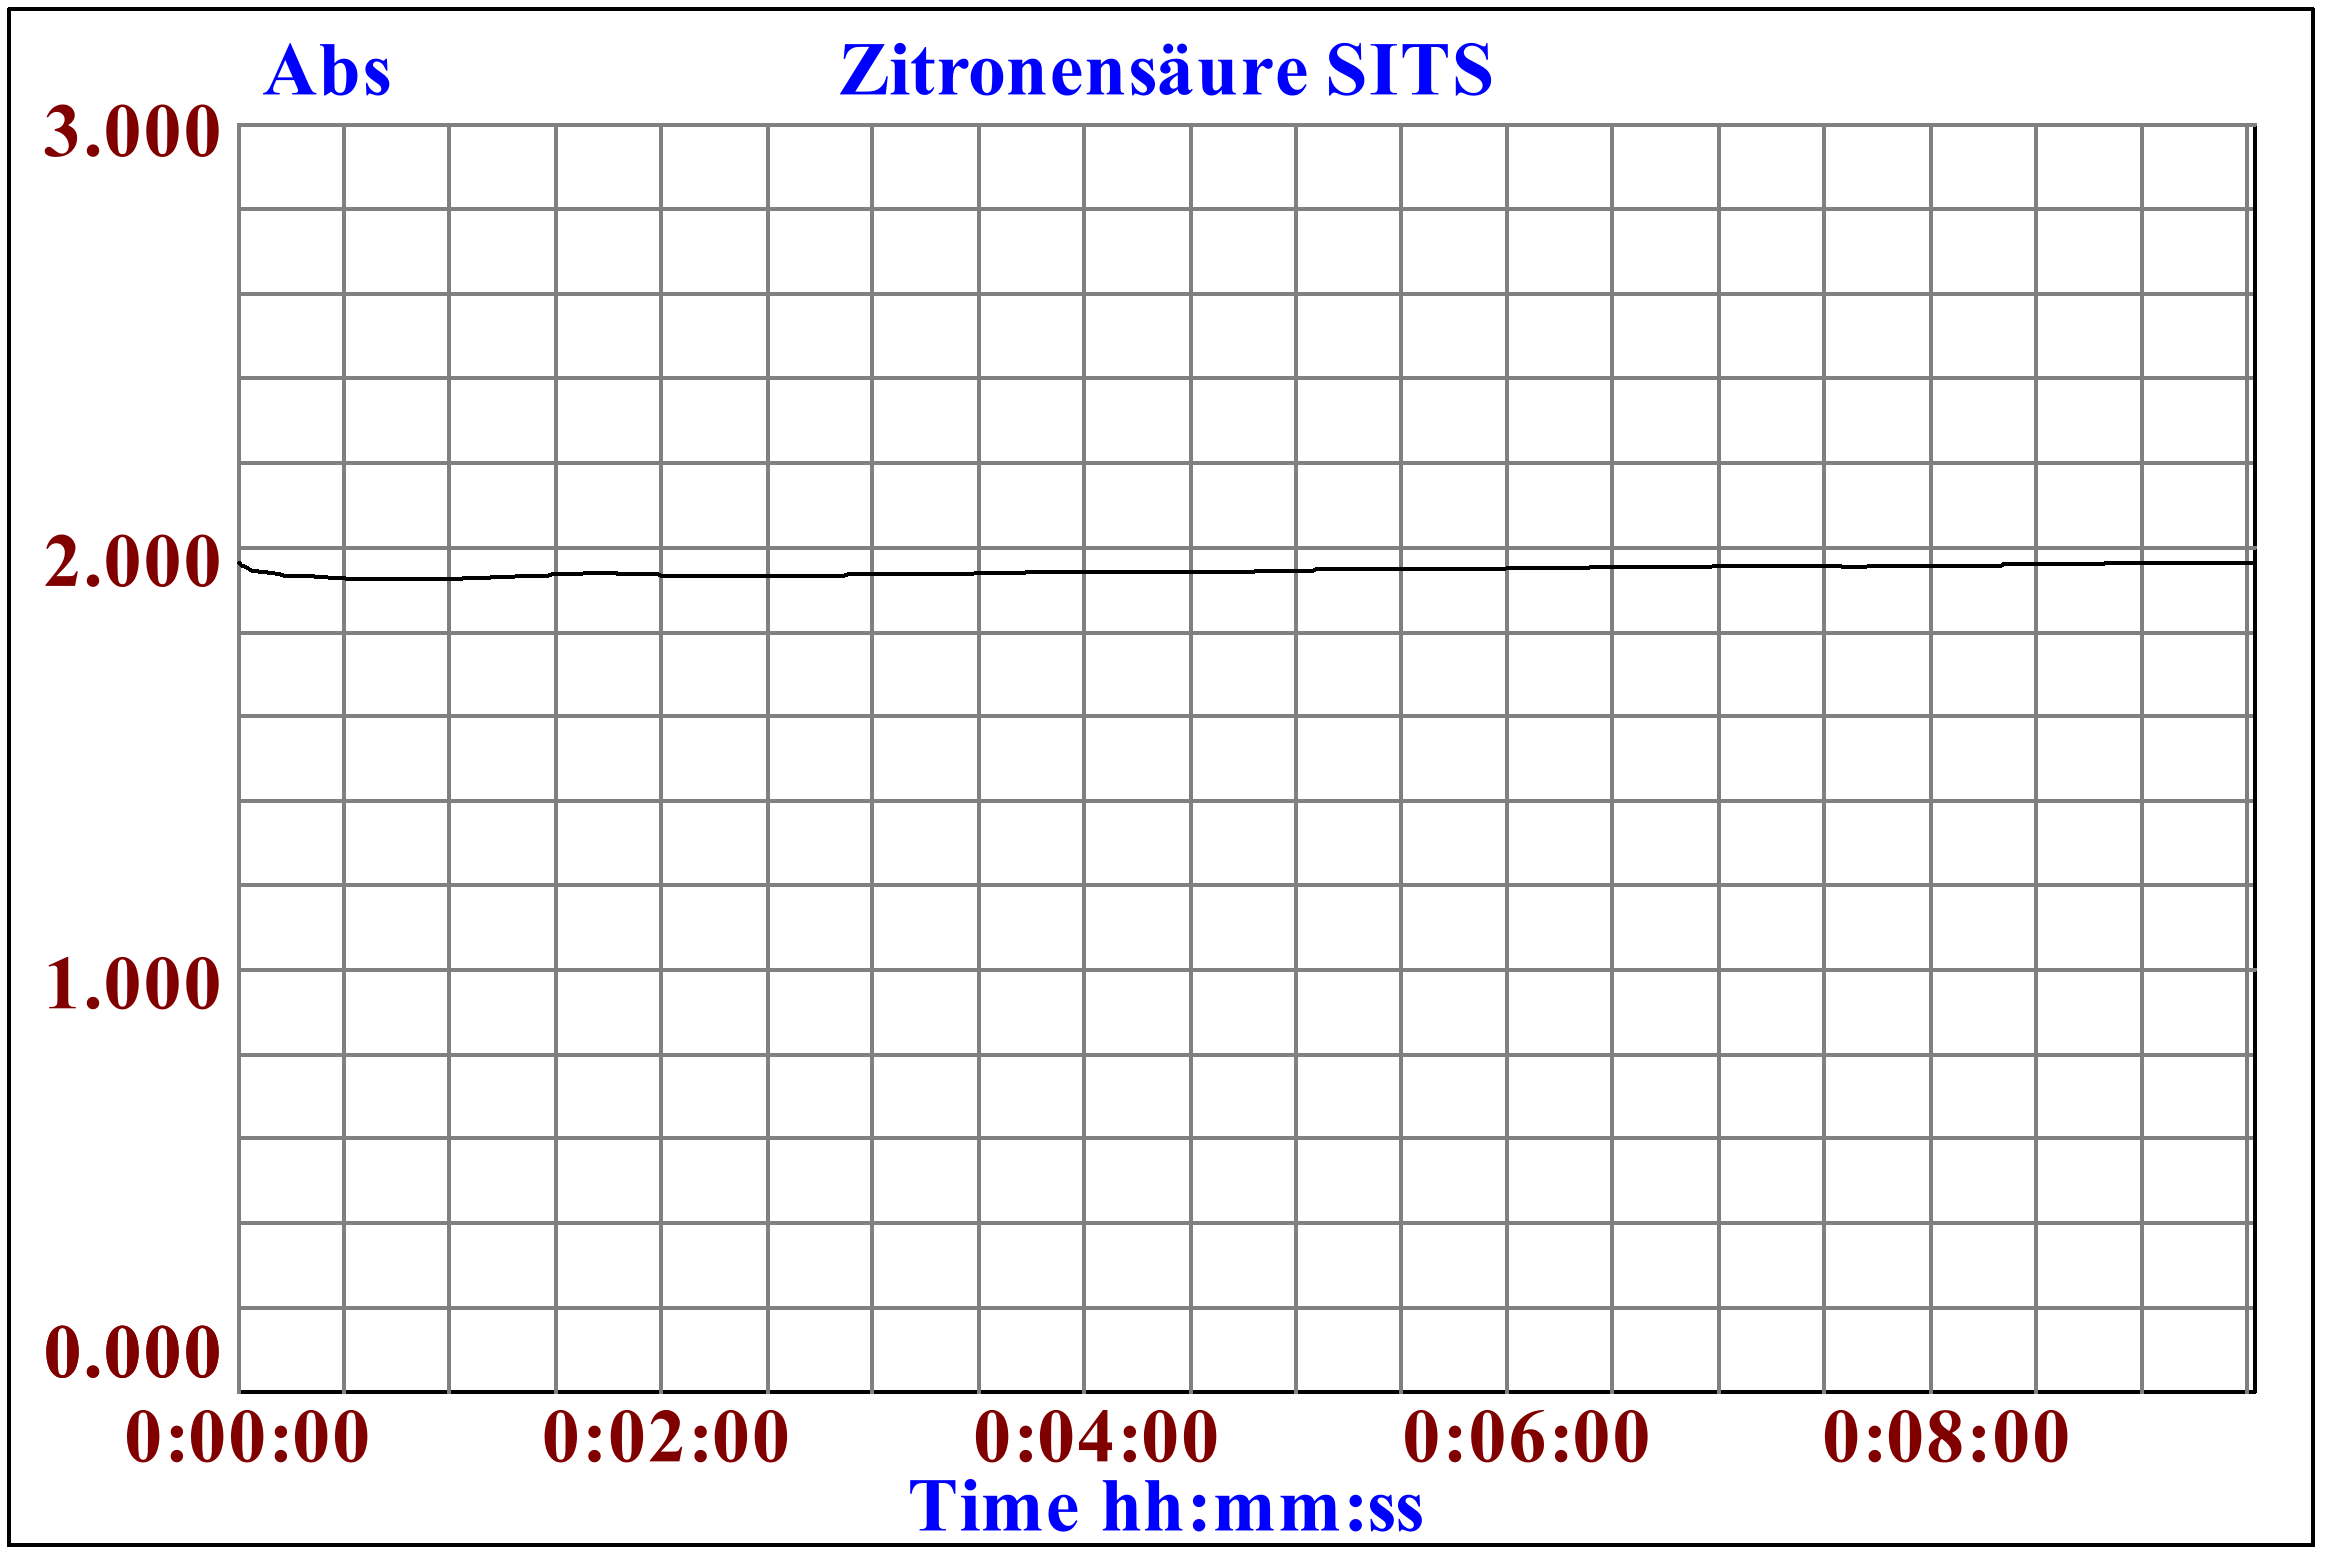
\includegraphics[width=\linewidth]{img/haem_citric_sits.png}
		\caption{Zitronensäure \& SITS}
	\end{subfigure}
	\caption{Absorption von Zitronensäure bei \SI{610}{nm}}
	\label{fig:haem_citric}
\end{figure}

\begin{figure}
	\centering
	\begin{subfigure}{.5\textwidth}
		\centering
		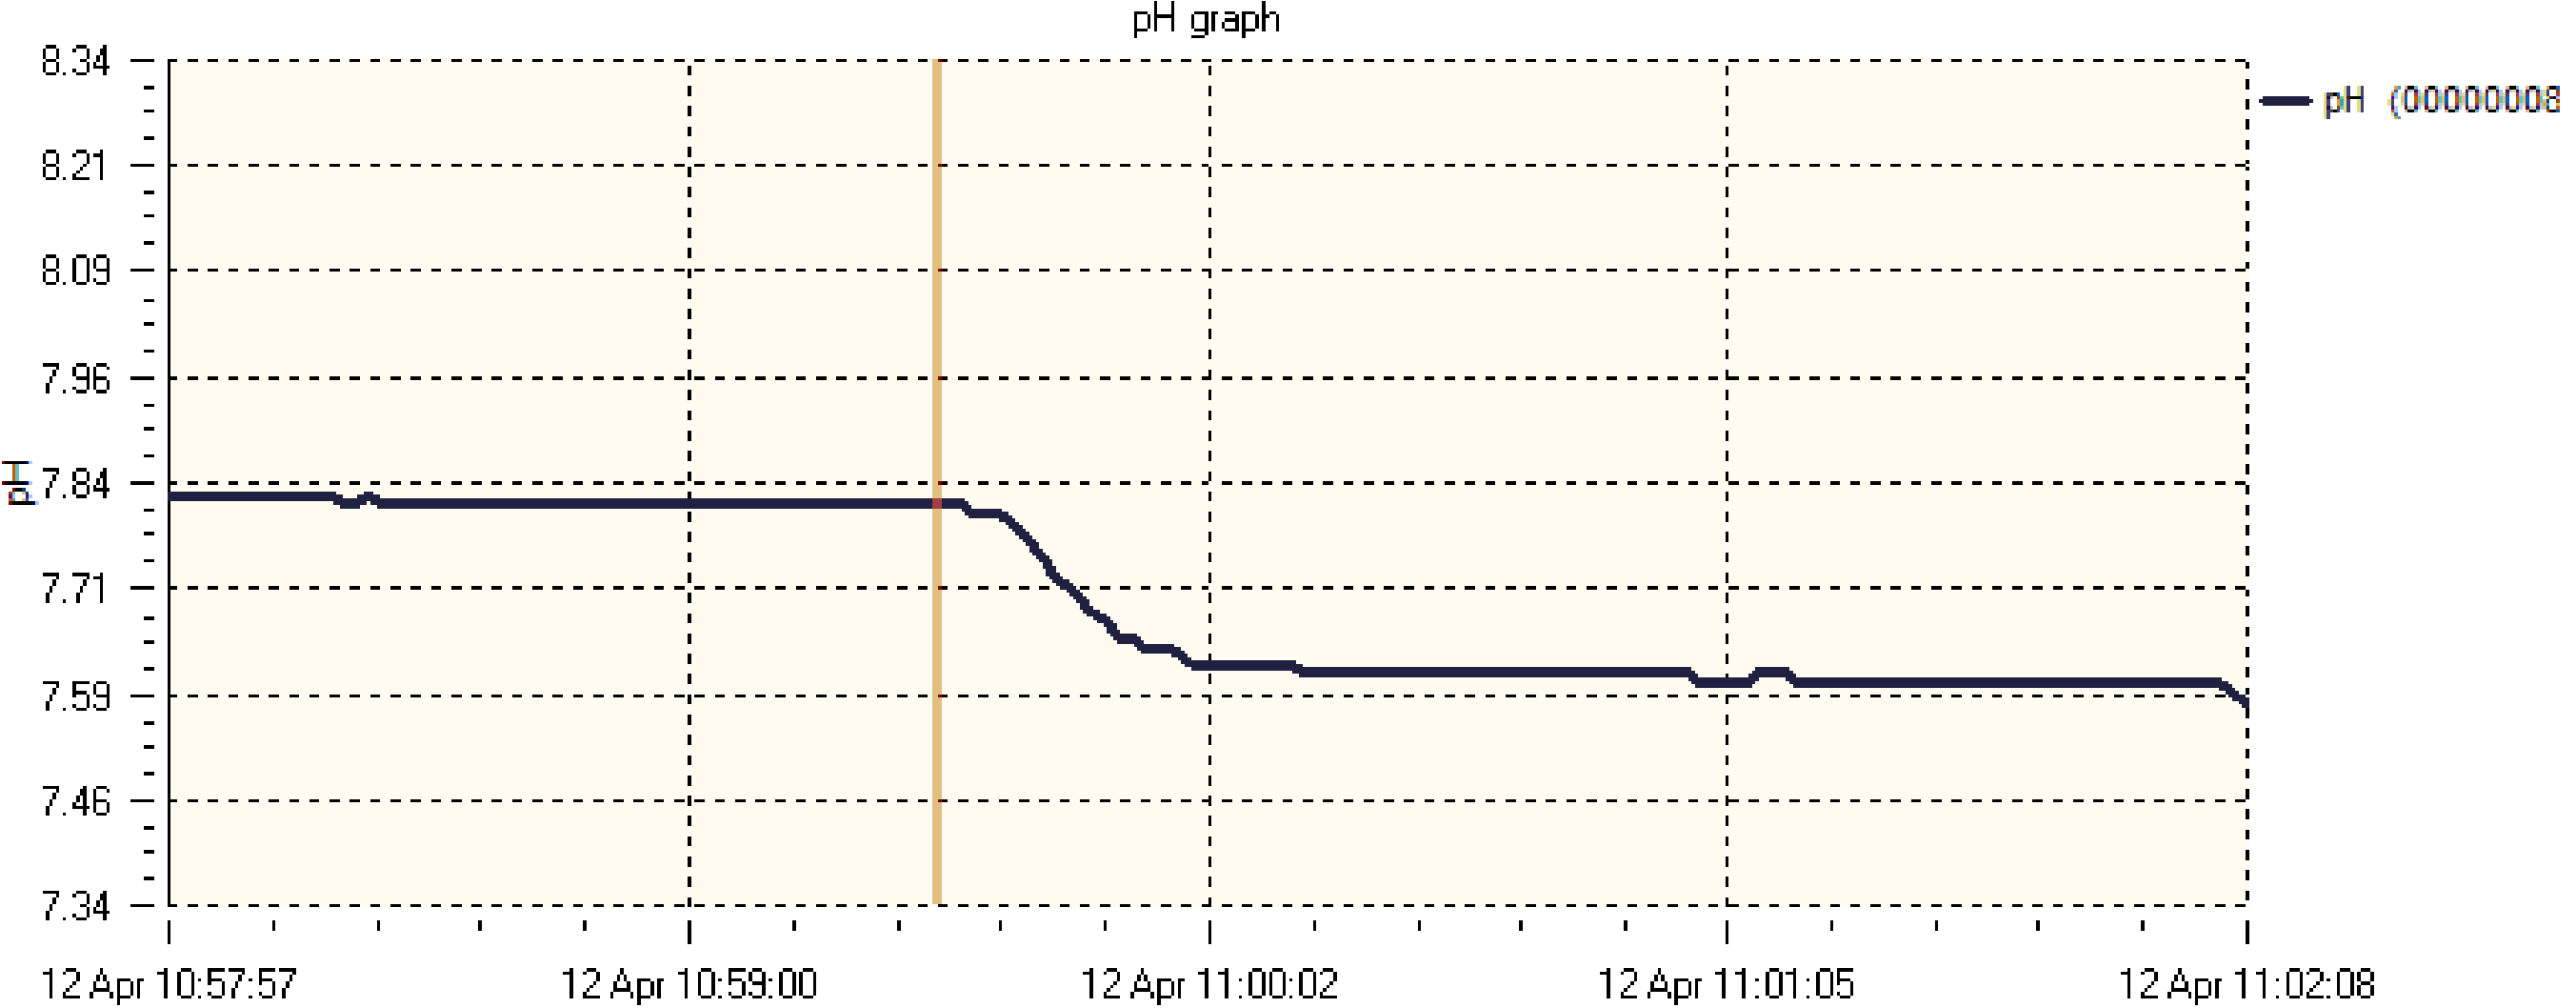
\includegraphics[width=\linewidth]{img/ph_citric.png}
		\caption{Zitronensäure}
	\end{subfigure}%
	\begin{subfigure}{.5\textwidth}
		\centering
		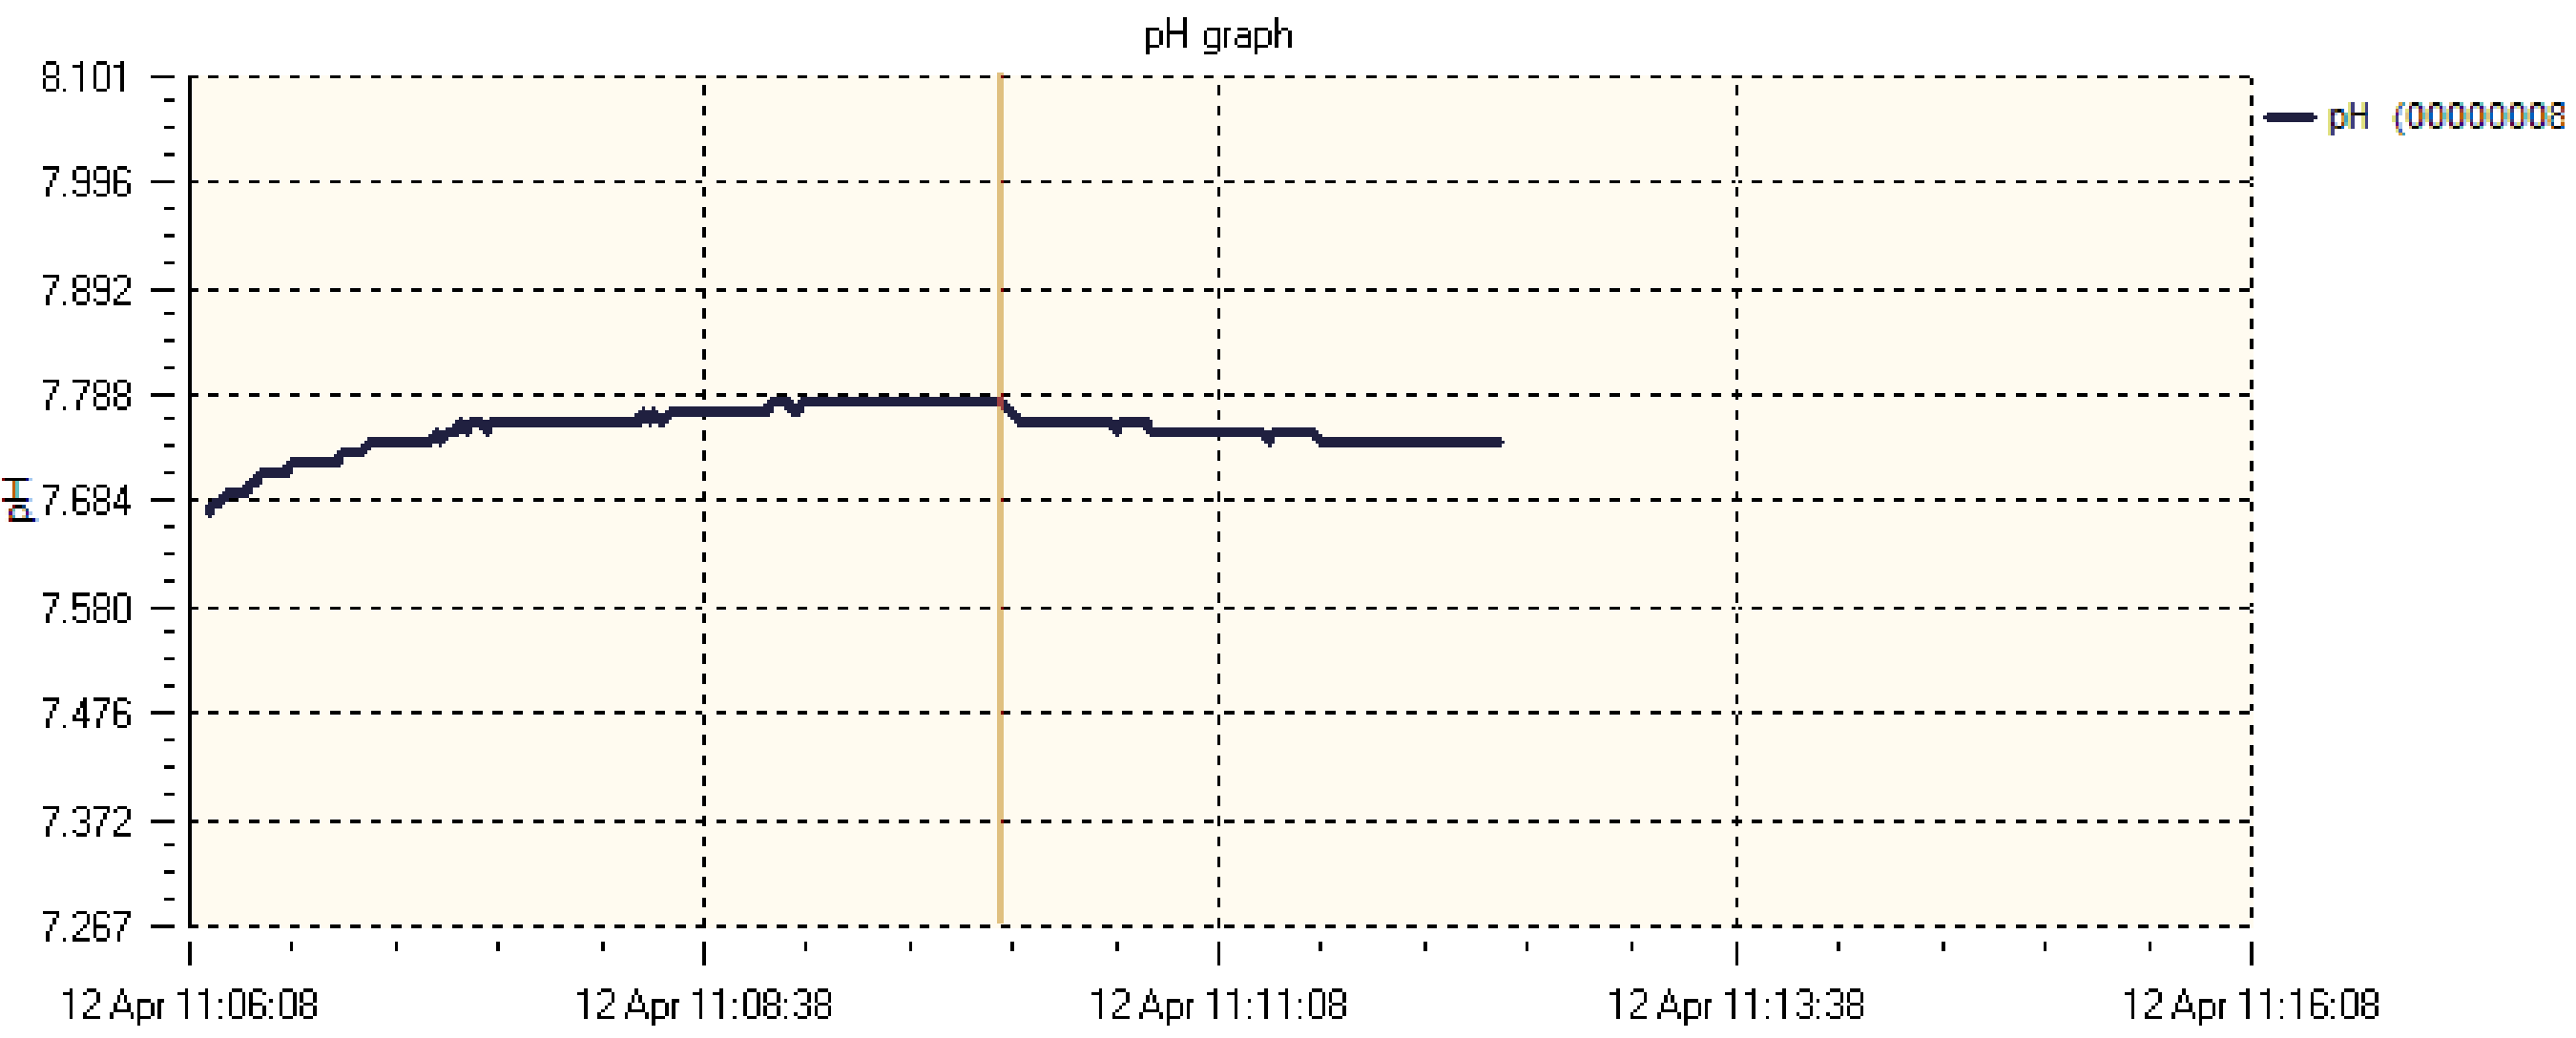
\includegraphics[width=\linewidth]{img/ph_citric_sits.png}
		\caption{Zitronensäure \& SITS}
	\end{subfigure}
	\caption{Extrazellulärer pH von Zitronensäure}
	\label{fig:ph_citric}
\end{figure}

Für die Zitronensäure gilt - analog der Weinsäure - dass anhand der
Absorptionsmessungen keine Hämolyse stattfindet, die Säure also weder via
Anionentransport noch via Diffusion die Zelle betritt.

Auch hier deckt sich diese Beobachtung mit der Messung des extrazellulären pH
Wertes.

\subsection{Natriumsalz der Essigsäure}

\begin{figure}[h]
	\centering
	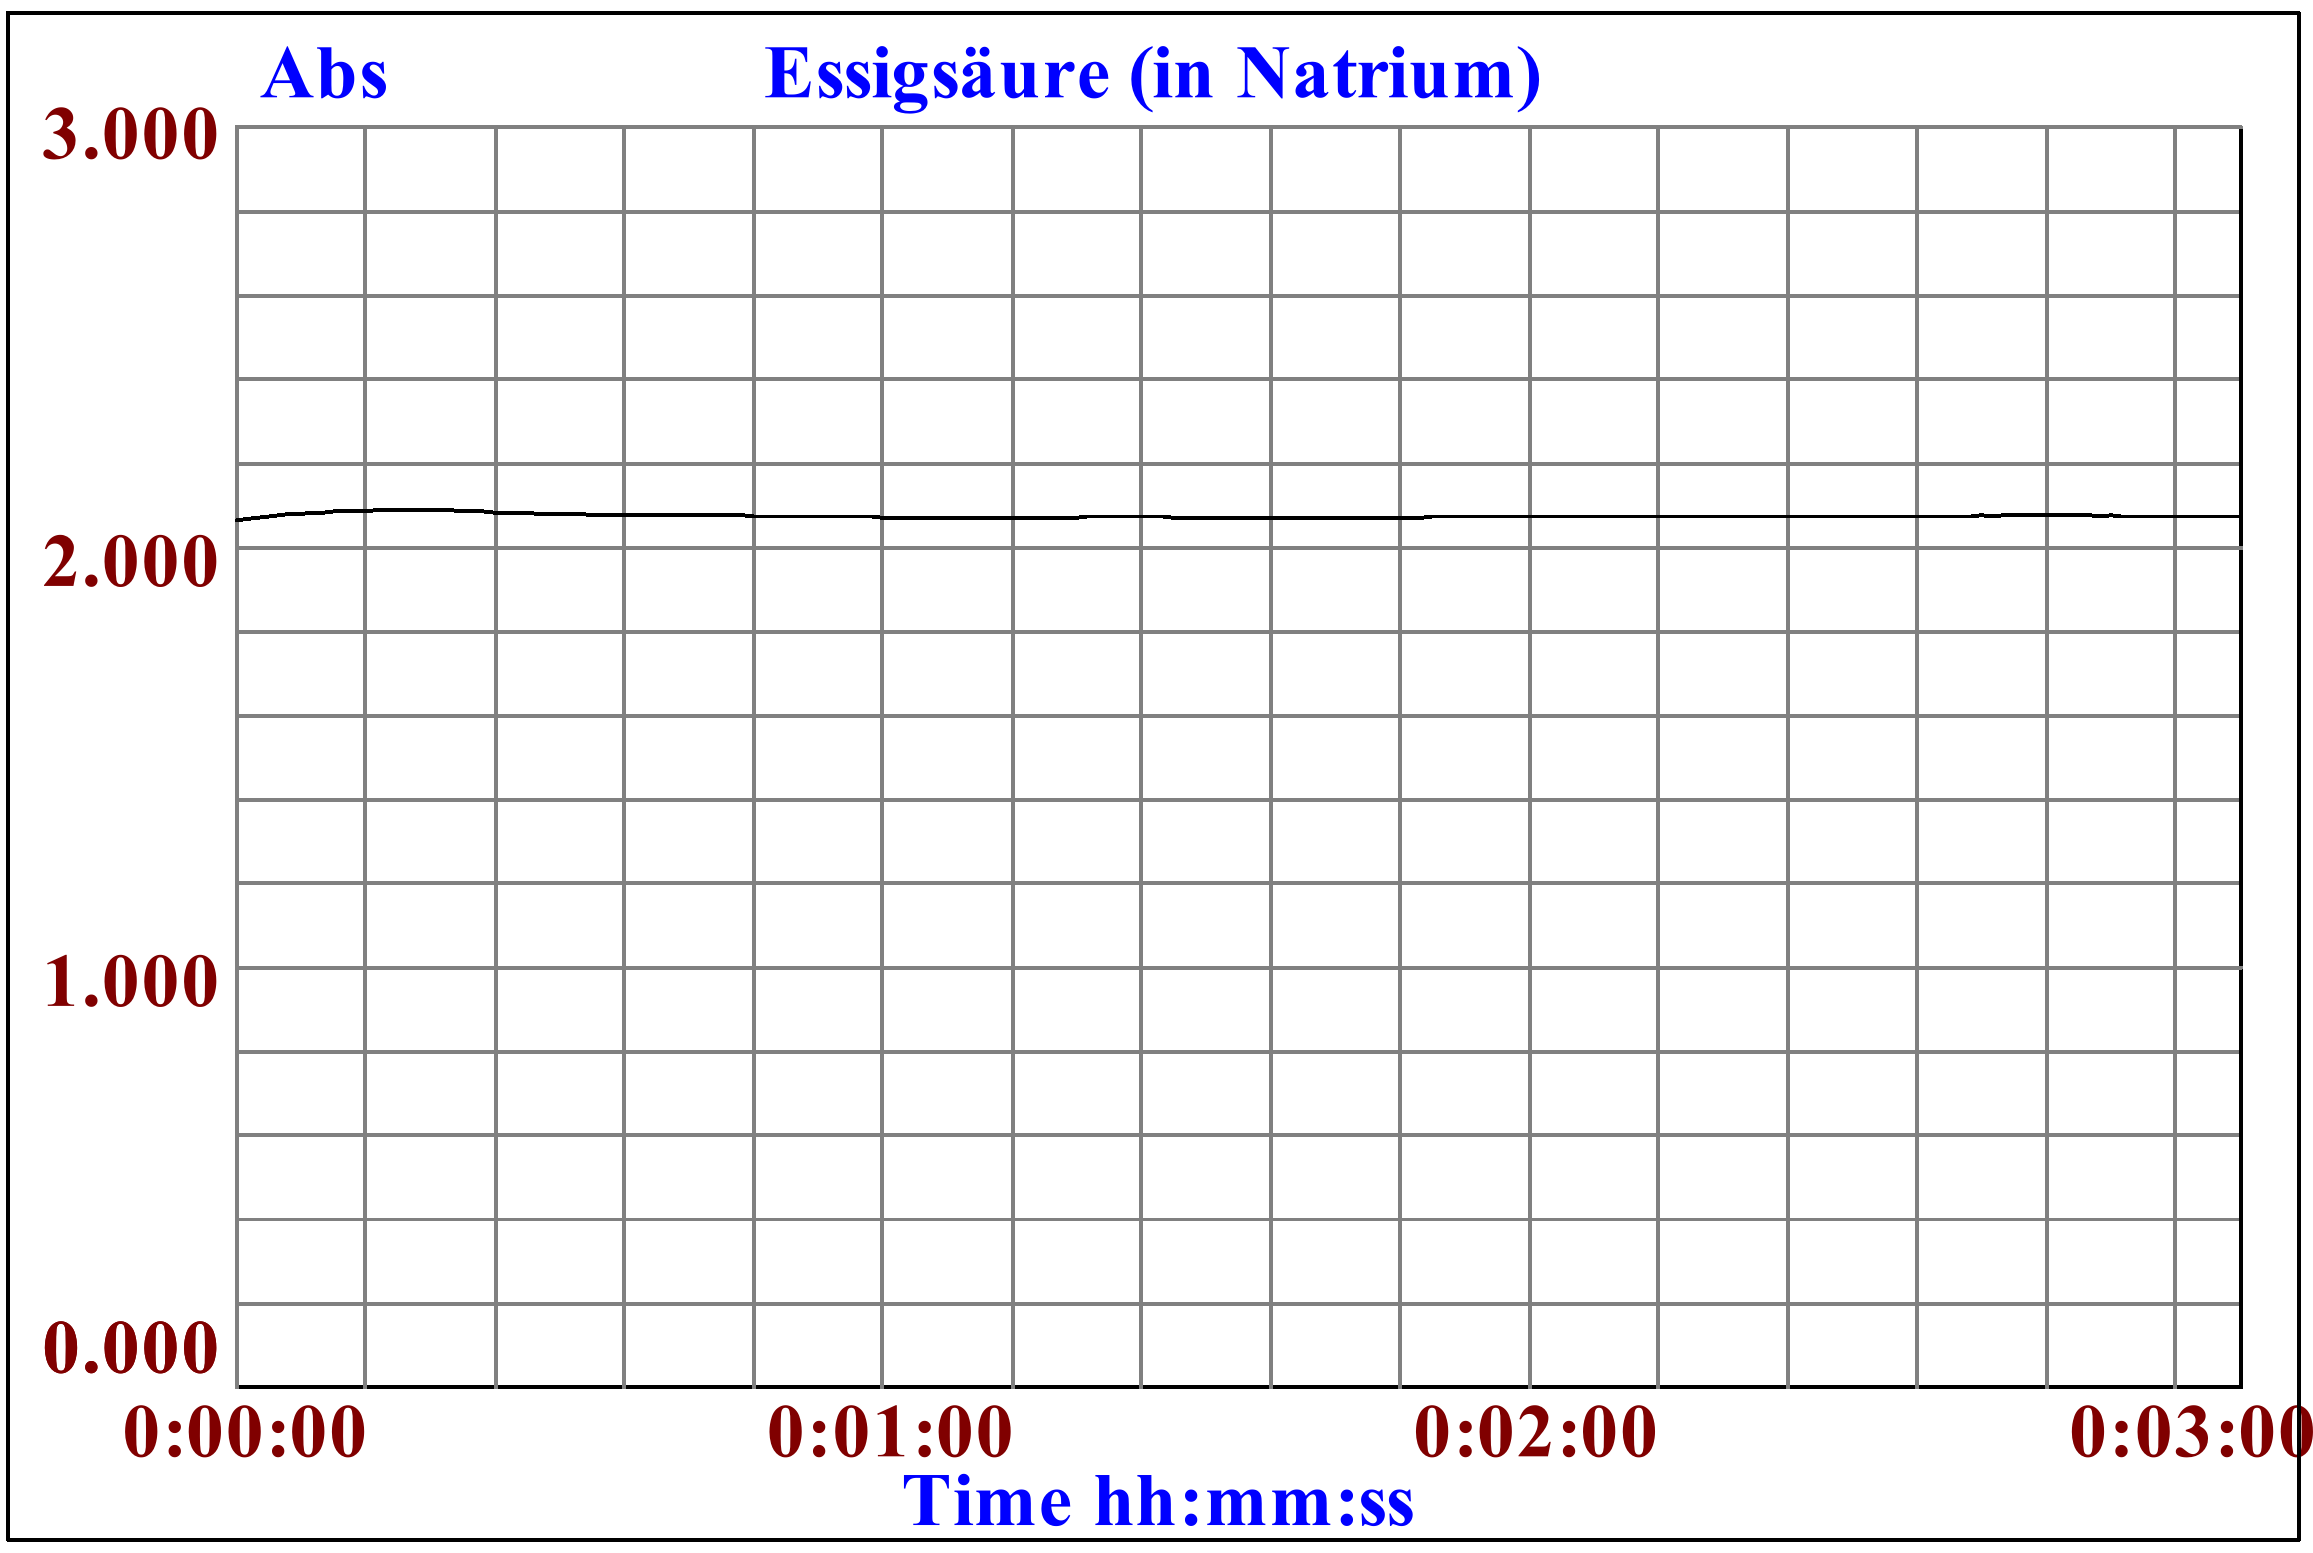
\includegraphics[width=0.5\textwidth]{img/haem_essig_na}
	\caption{Absorption von Essigsäure (Natriumsalz) bei \SI{610}{nm}}
	\label{fig:haem_essig_na}
\end{figure}

In Abbildung \ref{fig:haem_essig_na} ist ersichtlich dass das Natriumsalz der
Essigsäure zu keiner Hämolyse führte. Verglichen mit dem Ammoniumsalz der
Essigsäure - welches zu starker Hämolyse führte - ist damit klar, dass die
Hämolyse ein Resultat des Eindringens von \ce{NH3} ist.


\begin{landscape}
\section{Zusammenfassung}

Zusammenfassend lassen sich damit folgende Aussagen treffen.
\\

\begin{tabu}{lllllll}
	\toprule
	Säure & \multicolumn{2}{c}{Hämolyse} & Vermutete Transportart & pH Messung bestätigt & \multicolumn{2}{c}{Halbwertszeit} \\
	\cmidrule{2-3} \cmidrule{6-7}
	& Mit SITS & Ohne SITS & & & Mit SITS & Ohne SITS \\
	\midrule
	Ameisensäure  & Ja   & Minimal & Anionentransport & Nein & \SI{125}{s} & \SI{270}{s} \\
	Essigsäure    & Ja   & Ja      & Diffusion        & Ja   & \SI{60}{s}  & \SI{40}{s} \\
	Glyoxylsäure  & Ja   & Minimal & Anionentransport & Ja   & \SI{280}{s} & \SI{240}{s} \\
	Weinsäure     & Nein & Nein    & Kein Transport   & Ja   & -           & - \\
	Zitronensäure & Nein & Nein    & Kein Transport   & Ja   & -           & - \\
	\bottomrule
\end{tabu}
\end{landscape}

Zusammenfassend lassen sich deutliche Unterschiede in der Transportart und
Geschwindigkeit der verschiedenen organischen Säuren erkennen. Essigsäure als
kleines Molekül, mit polarem Kopf und apolarem Schwanz, ist in der Lage mit
hoher Geschwindigkeit durch die Membran zu diffundieren, während die
Ameisensäure oder Glyoxylsäure aufgrund des fehlenden apolaren Teils fast
exklusiv auf den Transport via Bande-3 Protein angewiesen sind.

Die Wein- und Zitronensäure können mangels fehlendem apolaren Teil ebenfalls
nicht durch die Membran diffundieren, und werden offensichtlich auch nicht
durch das Bande-3 Protein in die Zelle transportiert.

Interessant ist die deutlich kürzere Halbwertszeit der Ameisensäure verglichen
mit der Glyoxylsäure - potentiell begünstigt die kleinere Grösse der
Ameisensäure den Transport durch das Bande-3 Protein.

\section{Voraussage für Buttersäure}

\begin{figure}[h]
	\centering
	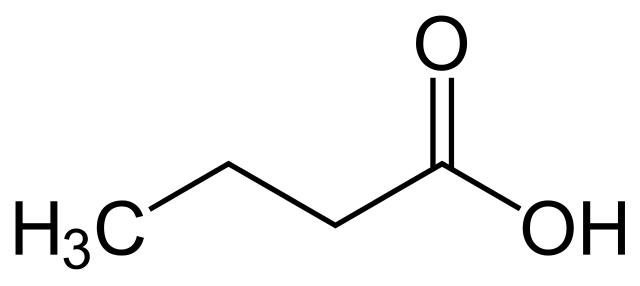
\includegraphics[width=0.4\textwidth]{img/buttersaeure}
	\caption{Struktur der Buttersäure}
	\label{fig:buttersaeure}
\end{figure}

Buttersäure - als Molekül mit einem polaren Kopf, und einem langen apolaren
Schwanz - wird vermutlich in der Lage sein durch die Membran zu diffundieren
ohne auf Transport durch das Bande-3 Protein angewiesen zu sein.


\bibliographystyle{plain}
\bibliography{references}

\end{document}
